% main.tex
%!TEX root = main.tex
% header.tex

\documentclass[a4paper,11pt,twoside,ngerman,color]{book}
\usepackage[a4paper,left=3.5cm,right=2.5cm,bottom=3.5cm,top=3cm]{geometry}

\usepackage[german,english]{babel}

\usepackage[pdftex]{graphicx,color}
\usepackage{amsmath,amssymb,subfigure}


% Theorem-Umgebungen
\usepackage[amsmath,thmmarks]{ntheorem}

% Korrekte Darstellung der Umlaute
\usepackage[utf8]{inputenc}
\usepackage[T1]{fontenc}

% Algorithmen
\usepackage[plain,chapter]{algorithm}
\usepackage{algorithmic}

\usepackage{enumerate}

\usepackage{float}

% Bibtex deutsch
\usepackage{bibgerm}

% URLs
\usepackage{url}

% Caption Packet
\usepackage[margin=0pt,font=small,labelfont=bf]{caption}
% Gliederung einstellen
%\setcounter{secnumdepth}{5}
%\setcounter{tocdepth}{5}

% Theorem-Optionen %
\theoremseparator{.}
\theoremstyle{change}
\newtheorem{theorem}{Theorem}[section]
\newtheorem{satz}[theorem]{Satz}
\newtheorem{lemma}[theorem]{Lemma}
\newtheorem{korollar}[theorem]{Korollar}
\newtheorem{proposition}[theorem]{Proposition}
% Ohne Numerierung
\theoremstyle{nonumberplain}
\renewtheorem{theorem*}{Theorem}
\renewtheorem{satz*}{Satz}
\renewtheorem{lemma*}{Lemma}
\renewtheorem{korollar*}{Korollar}
\renewtheorem{proposition*}{Proposition}
% Definitionen mit \upshape
\theorembodyfont{\upshape}
\theoremstyle{change}
\newtheorem{definition}[theorem]{Definition}
\theoremstyle{nonumberplain}
\renewtheorem{definition*}{Definition}
% Kursive Schrift
\theoremheaderfont{\itshape}
\newtheorem{notation}{Notation}
\newtheorem{konvention}{Konvention}
\newtheorem{bezeichnung}{Bezeichnung}
\theoremsymbol{\ensuremath{\Box}}
\newtheorem{beweis}{Beweis}
\theoremsymbol{}
\theoremstyle{change}
\theoremheaderfont{\bfseries}
\newtheorem{bemerkung}[theorem]{Bemerkung}
\newtheorem{beobachtung}[theorem]{Beobachtung}
\newtheorem{beispiel}[theorem]{Beispiel}
\newtheorem{problem}{Problem}
\theoremstyle{nonumberplain}
\renewtheorem{bemerkung*}{Bemerkung}
\renewtheorem{beispiel*}{Beispiel}
\renewtheorem{problem*}{Problem}

% Algorithmen anpassen %
\renewcommand{\algorithmicrequire}{\textit{Eingabe:}}
\renewcommand{\algorithmicensure}{\textit{Ausgabe:}}
\floatname{algorithm}{Algorithmus}
\renewcommand{\listalgorithmname}{Algorithmenverzeichnis}
\renewcommand{\algorithmiccomment}[1]{\color{grau}{// #1}}

% Zeilenabstand einstellen %
\renewcommand{\baselinestretch}{1.25}
% Floating-Umgebungen anpassen %
\renewcommand{\topfraction}{0.9}
\renewcommand{\bottomfraction}{0.8}
% Abkuerzungen richtig formatieren %
\usepackage{xspace}
\newcommand{\vgl}{vgl.\@\xspace} 
\newcommand{\zB}{z.\nolinebreak[4]\hspace{0.125em}\nolinebreak[4]B.\@\xspace}
\newcommand{\bzw}{bzw.\@\xspace}
\newcommand{\dahe}{d.\nolinebreak[4]\hspace{0.125em}h.\nolinebreak[4]\@\xspace}
\newcommand{\etc}{etc.\@\xspace}
\newcommand{\evtl}{evtl.\@\xspace}
\newcommand{\ggf}{ggf.\@\xspace}
\newcommand{\bzgl}{bzgl.\@\xspace}
\newcommand{\so}{s.\nolinebreak[4]\hspace{0.125em}\nolinebreak[4]o.\@\xspace}
\newcommand{\iA}{i.\nolinebreak[4]\hspace{0.125em}\nolinebreak[4]A.\@\xspace}
\newcommand{\sa}{s.\nolinebreak[4]\hspace{0.125em}\nolinebreak[4]a.\@\xspace}
\newcommand{\su}{s.\nolinebreak[4]\hspace{0.125em}\nolinebreak[4]u.\@\xspace}
\newcommand{\ua}{u.\nolinebreak[4]\hspace{0.125em}\nolinebreak[4]a.\@\xspace}
\newcommand{\og}{o.\nolinebreak[4]\hspace{0.125em}\nolinebreak[4]g.\@\xspace}
\newcommand{\oBdA}{o.\nolinebreak[4]\hspace{0.125em}\nolinebreak[4]B.\nolinebreak[4]\hspace{0.125em}d.\nolinebreak[4]\hspace{0.125em}A.\@\xspace}
\newcommand{\OBdA}{O.\nolinebreak[4]\hspace{0.125em}\nolinebreak[4]B.\nolinebreak[4]\hspace{0.125em}d.\nolinebreak[4]\hspace{0.125em}A.\@\xspace}

% Leere Seite ohne Seitennummer, naechste Seite rechts
\newcommand{\blankpage}{
 \clearpage{\pagestyle{empty}\cleardoublepage}
}

% Keine einzelnen Zeilen beim Anfang eines Abschnitts (Schusterjungen)
\clubpenalty = 10000
% Keine einzelnen Zeilen am Ende eines Abschnitts (Hurenkinder)
\widowpenalty = 10000 \displaywidowpenalty = 10000
% EOF

\begin{document}
\selectlanguage{german}
\begin{titlepage}
\definecolor{TUGreen}{rgb}{0.517,0.721,0.094}
\vspace*{-2cm}
\newlength{\links}
\setlength{\links}{-1.5cm}
\sffamily
\hspace*{\links}
\begin{minipage}{12.5cm}

\includegraphics[width=8cm]{bilder/tud_logo_rgb}
%\hspace*{-0.25cm} \textbf{TECHNISCHE UNIVERSIT"AT DORTMUND}\\
%\hspace*{-1.2cm} \rule{5mm}{5mm} \hspace*{0.1cm} FACHBEREICH INFORMATIK\\
\end{minipage}

\vspace*{4cm}

\hspace*{\links}
\hspace*{-0.2cm}
\begin{minipage}{9cm}
\large
\begin{center}
{\Large Bachelorarbeit} \\
\vspace*{1cm}
\textbf{Entwicklung einer Methodik zur optischen Analyse
spannkraftinduzierter Deformationen additiv gefertigter Bauteile} \\
\vspace*{1cm}
Niklas Thieme\\
% \vspace*{1cm}
\today
\end{center}
\end{minipage}
\normalsize
\vspace*{5.5cm}

% \hspace*{\links}

\vspace*{2.1cm}

\hspace*{\links}
\begin{minipage}[b]{10cm}
% \normalsize
\raggedright
Gutachter: \\
Prof. Dr.-Ing. Petra Wiederkehr \\
Melina Wenzel, M.Sc. \\
\end{minipage}

\vspace*{2.5cm}
\hspace*{\links}
\begin{minipage}[b]{8cm}
% \normalsize
\raggedright
Technische Universit"at Dortmund \\
Fakult"at f"ur Informatik\\
Virtual Machining (14)\\
https://vm.cs.tu-dortmund.de/
\end{minipage}


\end{titlepage}

\blankpage
\pagenumbering{roman}
\tableofcontents
\cleardoublepage
\pagenumbering{arabic}
% Kapitel
% 1_EinleitungMotivation_tex
\chapter{Einleitung}

In den letzten Jahren hat die additive Fertigung (AF), auch bekannt als 3D-Druck, 
zunehmend an Bedeutung in der Industrie gewonnen~\cite{JADHAV20222094}. 
Diese innovative Technologie 
ermöglicht die schichtweise Herstellung komplexer Bauteilgeometrien und bietet im 
Vergleich zu traditionellen Fertigungsverfahren einen höheren Grad an 
Gestaltungsfreiheit. Trotz dieser Vorteile stehen Hersteller vor 
Herausforderungen bezüglich der Oberflächenqualität und Maßhaltigkeit 
der gefertigten Werkstücke~\cite{SCHNECK201919}.
Herausforderungen können die Bauteilgeometrie, die möglichen Materialien oder 
den Herstellungsprozess betreffen.
Die Herausforderungen bei der Bauteilgeometrie umfassen die minimalen 
Wandstärken sowie das maximale Bauteilvolumen, das von den technischen 
Spezifikationen des verwendeten 3D-Druckers abhängt. Für das (AF) stehen 
verschiedene Materialien zur Verfügung, 
die sich jedoch von den in der konventionellen, spanenden Fertigung 
verwendeten Werkstoffen unterscheiden. In der AF werden hauptsächlich Legierungen 
auf Basis von Titan, Aluminium, Nickel oder Chrom eingesetzt. Diese Materialien
müssen zudem in einer für das Verfahren geeigneten Form vorliegen, 
meistens in Form von Pulver oder Draht. Der Prozess zur Herstellung von 
Pulver oder Draht aus diesen Materialien ist kostenintensiv und schränkt
die Auswahl der verwendbaren Materialien ein. Aufgrund der 
schichtbasierten Natur der AF sind Stützstrukturen 
notwendig, um Bauteile mit geometrischen Formen, die Überhänge aufweisen, 
erfolgreich produzieren zu können. \label{drawbacks_af}
\cite{Vranic.2017}

Einige dieser Herausforderungen, können durch Nachbearbeitung des Bauteils 
gelöst werden. Dazu gehört das Entfernen der Stützstrukturen und die Verbesserung
der Oberflächenqualität.
Für den Nachbearbeitungsschritt muss das Bauteil in seiner Position und Lage im Bauraum
der Werkzeugmaschine fixiert werden. Die hierzu aufzubringenden Spannkräfte 
können die filigranen Bauteile elastisch, in Extremfallen auch plastisch, verformen, 
sodass eine maßhaltige spangebende Nachbearbeitung verhindert wird. 
Um den Spannprozess und dessen Auswirkungen auf das Bauteil hinsichtlich 
der erzielbaren geometrischen Genauigkeit optimieren zu
können, ist eine Quantifizierung der spannkraftinduzierten Deformation notwendig.~\cite{newMethod}

Im Rahmen dieser Bachelorarbeit wird deshalb eine Methodik zum Erkennen und 
analysieren einer Deformation entwickelt. Das Ziel dieser Methodik ist es, 
mithilfe von optischen Informationen zu additiv gefertigten Bauteilen eine 
Deformation zu erkennen, wie sie zum Beispiel auftreten kann, wenn ein Bauteil 
in einem Schraubstock fixiert wird.

Das Verfahren soll auf verschiedenen Bauteilgeometrien anwendbar sein, daher werden 
möglichst wenig Annahmen über die Bauteilgeometrie getroffen.
Im Verlauf dieser Arbeit werden erst die theoretischen Grundlagen, die für die 
entwickelte Methodik notwendig sind dargestellt. 
Anschließend wird das Vorgehen der Methodik vorgestellt und die einzelnen 
Schritte erläutert. Das Verfahren besteht aus mehreren Schritten die sich in 
Datenerfassung, Datenaufbereitung, Stitchting und Deformationserkennung 
einteilen lassen.

Nach der Vorstellung des Verfahrens wird die Funktion der Methodik anhand eines 
Demonstratorbauteils das in einem Schraubstock fixiert und mit mehrere Kraftstufen 
angezogen wurde, validiert. Hier wird die erkannte Deformation bewertet und 
verschiedene Materialien und Herstellungsverfahren verglichen.

Ziel dieser Arbeit ist es zusätzlich, die entwickelte Methodik in einer einfach
benutzbaren Anwendung um zusetzten. Die Funktionsweise dieser Anwendung wird 
nach der Validierung der Methodik dokumentiert. Außerdem werden verschiedene 
Optimierungen dargelegt, die das Verfahren Zeit- und Speichereffizienter machen
und die Genauigkeit der Ergebnisse verbessern.

Zum Abschluss dieser Arbeit wird ein Fazit gezogen, in dem die erzielten 
Ergebnisse eingehend diskutiert werden. Zudem wird ein Ausblick auf 
mögliche zukünftige Entwicklungen und weiterführende Forschungsansätze gegeben.




\chapter{Grundlagen und Stand der Technik}

Für den Prozess der Deformationserkennung sind grundlegende Kenntnisse der 
Additiven Fertigung sowie des 3D-Designs von Vorteil. In diesem Kapitel 
werden sowohl diese Grundlagen als auch der aktuelle Stand der Technik 
erläutert.

\section{Additive Fertigung}

Additive Fertigung (AF) ist unabhängig von dem Werkstoff ein Bereich, in dem viel
geforscht und innoviert wird. In fast jedem Industriebereich wird versucht, ein
bestehendes Design oder Modell zu optimieren und zu verbessern.
Sei es hinsichtlich Qualität oder Kosteneffizienz. AF bietet bei 
dieser Optimierung viele Vorteile gegenüber spanenden Fertigungsverfahren, da 
AF einen höheren Grad der Gestaltungsfreiheit bietet. 
AF ist eine Ressource, welche Benutzern ermöglicht, komplexe 
Bauteilgeometrien zu erstellen, ohne die Limitierung von konventionellen spanenden 
Herstellungsverfahren zu erstellen. 
Limitierungen von konventionellen spanenden 
Herstellungsverfahren kann ein hoher Materialverschleiß oder die Notwendigkeit von 
spezialisierten Werkzeugen sein.\ \cite{Vafadar.2021} 

Außerdem können mit additiver Fertigung Stückzahlen drastisch reduziert werden.
Werkstücke können bei Bedarf gefertigt werden, was die Notwendigkeit für Lagerstätten
größtenteils eliminiert. Zusätzlich können die Teile genau dort herstellt werden, wo 
sie benötigt werden, was Lieferketten und Wartezeiten verkürzt~\cite{Calignano.2023}.

Bauteile können mit verschiedenen Werkstoffen, darunter sind Polymeren, Metalle und Keramik, 
additiv gefertigt werden.
Metalle haben vor allem in den letzten Jahren 
an Relevanz gewonnen. Zusätzlich zu den schon genannten Vorteilen von AF, 
bietet Metall als Werkstoff großen Nutzen in der Industrie. Gegenüber Kunststoffen
produziert Metall weniger Abfall und kann eine höhere Qualität gewährleisten.
Zusätzlich dazu kommen die offensichtlichen Vorteile von Metall gegenüber Polymeren: 
höhere Hitzebeständigkeit und eine stabilere Grundstruktur, was sie weniger anfällig 
für Verformungen macht~\cite{Gardner.2023}.

Aufgrund dieser Vorteile wird AF in vielen Industriebereichen genutzt. Die folgende
Sektion zeigt einige Fälle in der Automobilindustrie, in denen AF 
erfolgreich benutzt wird.
Die Automobilbranche ist ein Bereich, in der AF schon viel und erfolgreich 
eingesetzt wird:
Durch AF könne Teile gefertigt werden, die leichter, belastbarer und sicherer sind. 
Die einfache Anpassbarkeit sorgt für geringe Entwicklungszeiten und Kosten. 
BWM zum Beispiel benutzt für den i8 Roadster viele AF gefertigte Teile.
Darunter sind zum Beispiel die Befestigung für das Soft-Top, die 44 \% leichter als das Spritzgussteil
ist, und dennoch zehnmal steifer.\ \cite{Vafadar.2021} 
Fensterführungen wurden auch additiv gefertigt. Mithilfe des \glqq HP Multi Jet Fusion\grqq~
konnten 
100 Teile in 24 Stunden gefertigt werden. Selbst Teile des Zylinderkopfs für den 
S58 Motor wurden additiv gefertigt. \cite{Anusci.2019}

Auch bei älteren Fahrzeugen können additive Fertigungsmethoden zur 
Reparatur oder Restauration verwendet werden.
Gerade bei älteren Fabrikaten sind Ersatzteile häufig nicht mehr vom 
Erstzulieferer zu beschaffen oder mit konventionellen Herstellungsmethoden
wirtschaftlich herzustellen.
Bei einem Matra 530 aus 1973 wurde zum Beispiel die rechte 
Kotflügelhalterung erfolgreich reproduziert, nachdem auch nach längerer Suche
kein Originalteil gefunden wurde \cite{AMExpo365.03.06.2024}. Zusätzlich war
bei diesem Beispiel die Herausforderung, das keine digitale Version des
Bauteils existiert hat. Zuerst musste also ein Modell als Grundlage für die
additive Fertigung erzeugt werden.

\section{Limitierungen von AF}

AF kann trotz seiner Vorteile nicht überall eingesetzt werden. Limitierungen 
in der Materialvielfalt, hohe Material und Anschaffungskosten, begrenzte
Bauraumgrößen, verminderte Oberflächenqualität und aufwändige Nachbearbeitungen
können einen Einsatz von AF verhindern beziehungsweise unwirtschaftlich machen. 
\cite{inproceedings}
Einige dieser Limitierungen können umgangen oder gelöst werden. 
Zum Beispiel kann die
verminderte Oberflächenqualität kann durch eine anschließende Fräsbearbeitung
verbessert werden. 
Diese Nachbearbeitung macht eine Fixierung des Bauteils notwendig. Auch für andere
Nachbearbeitungen wie das Entfernen von Stützstrukturen kann sich das fixieren
positiv auswirken und Zeit im Herstellungsprozess eingespart werden.
Wie schon in Kapitel \ref{drawbacks_af} beschrieben, sind 
Stützstrukturen notwendig, wenn das zu produzieren Bauteil Überhänge aufweist,
die eine Steigung von ungefähr 30° unterschreiten. Der Grad des Überhangs 
variiert je nach verwendetem Material und Verfahren.

\begin{figure}[H]
    \centering
    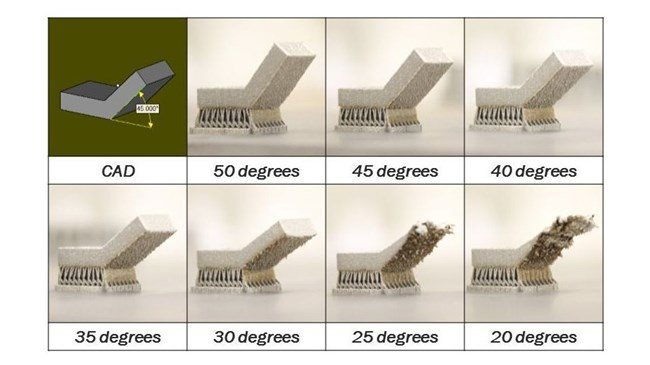
\includegraphics[width=0.9\linewidth]{images/Overhang-tests-showing-different-printabilities-and-finish-qualities-at-seven-different.jpg}
    \caption{Überhangtests mit unterschiedlichen Resultaten und 
    Oberflächenqualitäten in sieben verschiedenen Winkeln \cite{Meng.2020}}
    \label{fig:overhang}
\end{figure}

\section{Reverse Engineering}

Reverse Engineering beschreibt den Prozess aus einem bestehenden Produkt 
oder Objekt ein digitales Abbild zu erzeugen.
Dabei sind meistens wenig oder keine technischen Details über das Objekt
verfügbar.~\cite{Helle.2021}  
Auch wenn Baupläne vorhanden sind, kann es trotzdem notwendig sein, 
Reverse Engineering zu betreiben, denn das tatsächliche Produkt kann von
den Bauplänen abweichen. Produkte und Bauteile können durch die Benutzung 
abgenutzt werden und entsprechen deswegen unter Umständen nicht mehr den originalen 
Bauplänen. Zusätzlich können Toleranzen im ursprünglichen Fertigungsprozess 
für Diskrepanzen sorgen. Wenn technische Details vorhanden sind,
können diese aber im Reverse Engineering Prozess verwendet werden.\ \cite{Monchinger.2021} 
Dieses Paper zeigt, wie Reverse Engineering genutzt werden kann, um 
bestehende Bauteile passgenau zu erweitern. Konkret geht es um die
Entwicklung einer Methodik um automatisiert Laser-Scans und originale Baupläne
zusammenzufügen um ein möglichst detailgetreues Abbild der realen Struktur zu
erzeugen. Dieses Abbild wird dann benutzt, um die bestehende Struktur zu 
erweitern und auf ihr aufzubauen. Das wird am Beispiel eines Flugzeugs 
demonstriert, erst wird der Innenraum gescannt und mit dem originalen Plänen
abgeglichen, dann ein 3D Objekt erstellt. Mithilfe dieses 3D-Objekts können 
dann passgenaue Bauteile hergestellt werden, die es ermöglichen ein ehemaliges 
Passierflugzeug in eine Frachtmaschine umzubauen.
Wie schon erwähnt, wird zur erfolgreichen Weiterbearbeitung ein möglichst 
genaues digitales Abbild benötigt.
Ist dies nicht der Fall, müssen nicht passende Teile erneut hergestellt werden, 
was die Material- und Personalkosten deutlich erhöht. Es ist also im 
wirtschaftlichen Interesse beim ersten Schritt, dem Erstellen der digitalen 
Version, ein möglichst genaues Ergebnis zu erzielen. 

\section{3D Rekonstruktion}

Digitale Abbildungen von Flächen, Objekten oder sogar Körperteilen wurden in den
letzten Jahren mehr benutzt. Anwendungen sind zum Beispiel in der
geometrischen Dokumentation, Inspektion, Navigation, Visualisierung und 
Objekterkennung zu finden~\cite{Verykokou.2023}. Je nach Anwendungsfall wird eine
bestimmte Genauigkeit
der Daten erwartet, im medizinischen Bereich sind die Ansprüche natürlich ganz 
andere als zum Beispiel in der Dokumentierung von ganzen Gebirgszügen.
Das Scannen von Gesichtstexturen zeigte Abweichungswerte zwischen 140 $\mu$m und 
1330 $\mu$m, während die 3D-Rekonstruktion des Kieferknochens Werte zwischen 106 $\mu$m 
und 760 $\mu$m aufwies. 
Das Scannen eines bezahnten Bogens durch intraorale und Labor-basierte
Scanner variierte zwischen 17 $\mu$m und 378 $\mu$m und bei der 
digitalen Abtastung von Zahnimplantaten zwischen 19,32 $\mu$m
und 112 $\mu$m~\cite{Bohner.2019}.
Bei Lidar-Scans eines Sportkomplexes wurde eine Standardabweichung von ±0.10 Metern
gemessen. Es wurde aus 600 Meter Höhe vermessen und die Scandaten mit 
Referenzpunkten auf dem Boden verglichen.~\cite{Elaksher.2023}
Aus diesem Grund existieren auch verschiedene Herangehensweisen und Technologien  
zur 3D-Rekonstruktion.

3D Rekonstruktion-Technologien können in 2 Kategorien eingeteilt werden,
die bildbasierte Verfahren und die Verfahren die auf Scandaten 
beruhen.~\cite{Verykokou.2023} [TODO es existieren noch mind. 2 weitere verfahren]
Beide Verfahren können auch kombiniert werden. 
Bei bildbasierten Verfahren, auch Fotogrammetrie genannt, wird das 3D Objekt aus
mehreren zweidimensionalen Bildern erstellt, 
umso mehr Bilder vorhanden sind, desto besser kann das
3D Objekt rekonstruiert werden. Um das 3D Objekt zu erstellen werden in 
allen Bildern gemeinsame Punkte gesucht und dann mit der bekannten Kameraposition, 
die relative Position des Punktes im 3D Objekt ermittelt. Figur [todo figur einfügen] zeigt dies 
anschaulich.
Vorteil bei der Fotogrammetrie ist, dass die Daten relativ einfach aufgenommen werden
können. Die Kamera eines Smartphones kann ausreichend hochauflösende Bilder aufnehmen, um 
eine 3D-Rekonstruktion zu ermöglichen. Des Weiteren sind viele Softwarelösungen,
auch kostenlose, vorhanden um automatisiert 3D Objekte zu erzeugen.
Gründe, sich gegen den Einsatz von Fotogrammetrie zu entscheiden, 
liegen in der begrenzten Auflösung sowie im signifikant ansteigenden Arbeitsaufwand 
bei steigenden Anforderungen an die Genauigkeit des Endergebnisses. 
Fotogrammetrie zeigt jedoch ihre Stärken bei großflächigen 3D-Rekonstruktionen, 
wie sie beispielsweise bei der Erfassung von Gebäuden, Stadtteilen oder geografischen 
Strukturen erforderlich sind.

\begin{figure}[H]
    \centering
    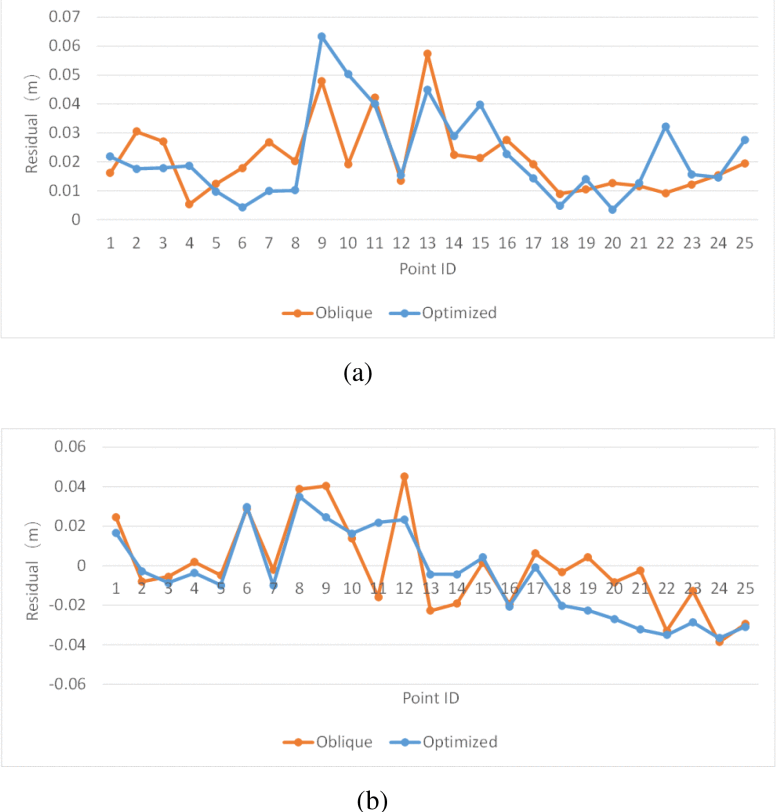
\includegraphics[width=\linewidth]{images/photogammatry_accurancy.PNG}
    \caption{Genauigkeit der Fotogrammetrie bei Bildern die aus 
    600 m Höhe aufgenommen wurden \cite{Elaksher.2023}.}
    \label{fig:photogammatryAccuracy}
\end{figure}

Für kleine Objekte, bei deren Rekonstruktion eine hohe Genauigkeit gefordert ist, 
sollte daher das zweite Verfahren angewendet werden. Bei diesem Verfahren werden
die Ursprungsdaten dreidimensional mit einem Scanner erfasst. Ein Scanner misst dabei, 
meist mithilfe von Lichtstrahlen, den Abstand zu einem Punkt auf dem zu 
rekonstruierenden Objekt. Um eine Vielzahl von Scanpunkten zu erfassen, 
wird entweder das Objekt oder der Scanner bewegt. Je mehr Punkte erfasst werden, 
desto genauer wird das Ergebnis. Allerdings nimmt die Datenmenge mit der Anzahl der 
Scanpunkte ebenfalls zu, was ab einem bestimmten Punkt zu einer Einschränkung durch den 
verfügbaren Speicher führen kann. Zudem steigt die Rechenzeit mit der Datenmenge an, 
und je nach angewendetem Verfahren kann dieser Anstieg sogar 
exponentiell sein~\cite{XiaoleiDu.2009}.

Nachteile von diesem Verfahren sind die hohen initialen Kosten eines Scanners 
und der begrenzte Messbereich. 

\subsection{Digitales Abbild}

Das schon vorhandene oder erstellte 3D Objekt muss für die weitere Nutzung
in einem geeigneten Datenformat gespeichert werden. Hierfür haben sich mehrere
Formate etabliert. Die Geometrie eines Objekts wird häufig als Sammlung von Punkten 
gespeichert. Die Oberfläche eines Objekts wird als Serie von Polygonen beschrieben. 
Der Grad des Polygons kann variieren, häufig werden Dreiecke verwendet. 
Die Genauigkeit, mit der das Polygon-Netz die gewünschte Oberfläche 
abbildet, kann gewählt werden. 
Je kleiner die Oberfläche der Polygonen ist, desto genauer wird die Oberfläche 
abgebildet. Mit kleineren Oberflächen steigt die Anzahl der zu speichernden 
Eckpunkte, was eine größere Datei zur Folge hat.
Ein in der akademischen Welt beliebtes Dateiformat für Polygon-Netze ist das 
Polygon File Format (ply).\ \cite{KentonMchenry.2008}
Das Format kann vom Nutzer beliebig angepasst werden. Eine ply-Datei beginnt mit 
einem Header in dem die Inhaltsstruktur beschrieben wird. 
Für 3D-Objekte besteht diese meistens aus X, Y und Z Koordinaten. 
Zusätzlich können weitere Informationen gespeichert werden. Das ply Dateiformat 
unterstützt standardmäßig: \glqq vertices/edges/faces, vertex colors, textures and
material \grqq ~\cite{KentonMchenry.2008}. Weitere Informationen können durch den Nutzer 
hinzugefügt werden, 
diese können dann aber unter Umständen nicht von anderen Programmen oder Benutzern
benutzt werden.
Im Dateiheader wird zu jedem Attribut auch der Datentyp festgelegt. Durch diesen 
kann die Genauigkeit und Dateigröße beeinflusst werden. Häufig werden hier Floats oder
Integer in verschiedener Bittiefe gewählt.

\begin{figure}[h]
    \centering
    \begin{minipage}{0.32\textwidth}
        \centering
        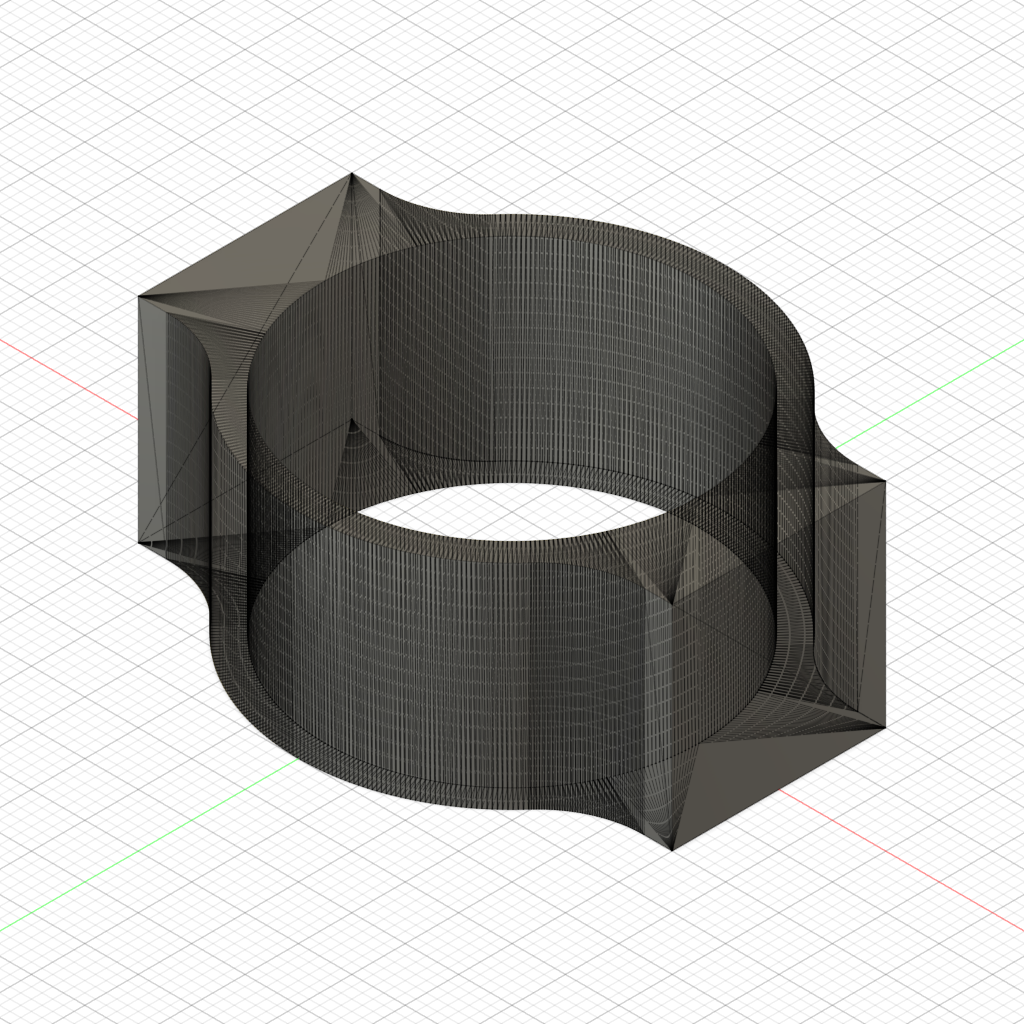
\includegraphics[width=\linewidth]{images/image_demo.PNG} % first figure itself
        \caption*{(a)}
    \end{minipage}\hfill
    \begin{minipage}{0.32\textwidth}
        \centering
        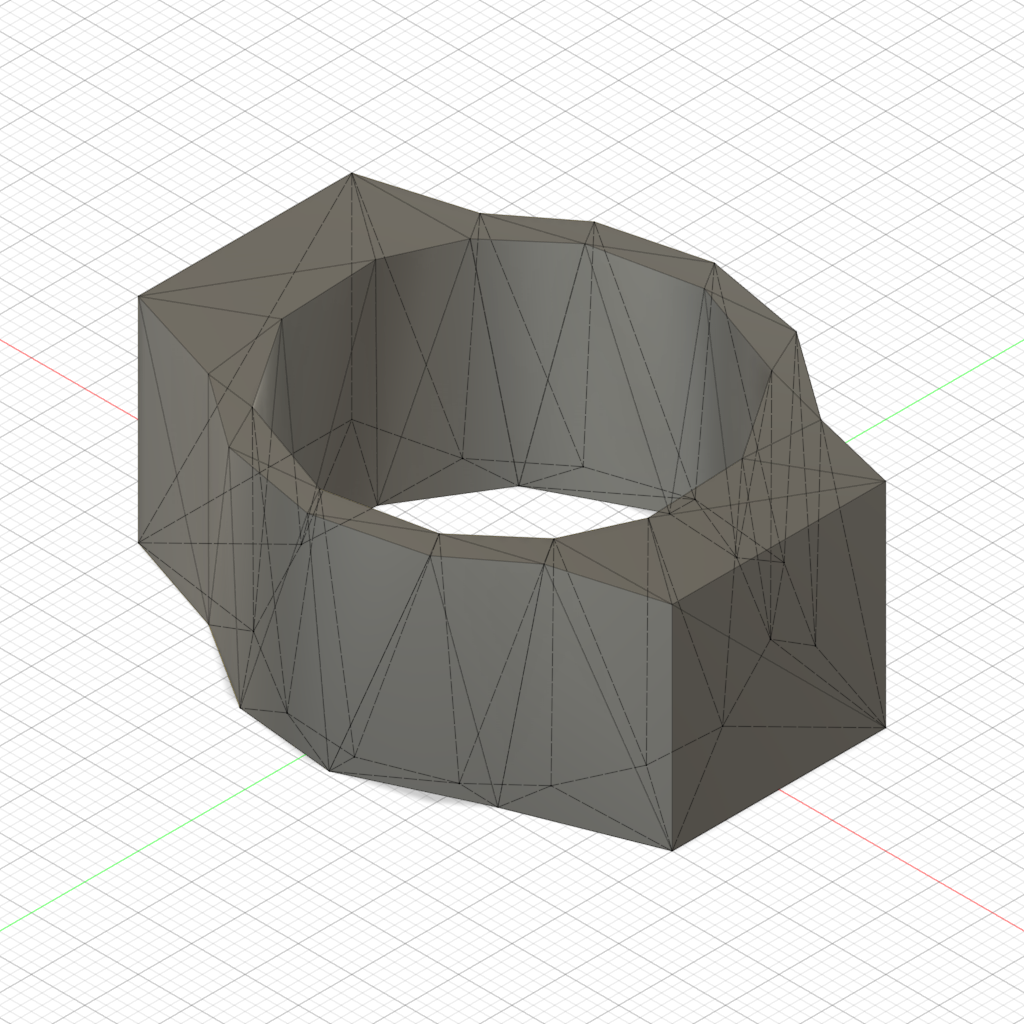
\includegraphics[width=\linewidth]{images/image_demo_medium.PNG} % first figure itself
        \caption*{(b)}
    \end{minipage}\hfill
    \begin{minipage}{0.32\textwidth}
        \centering
        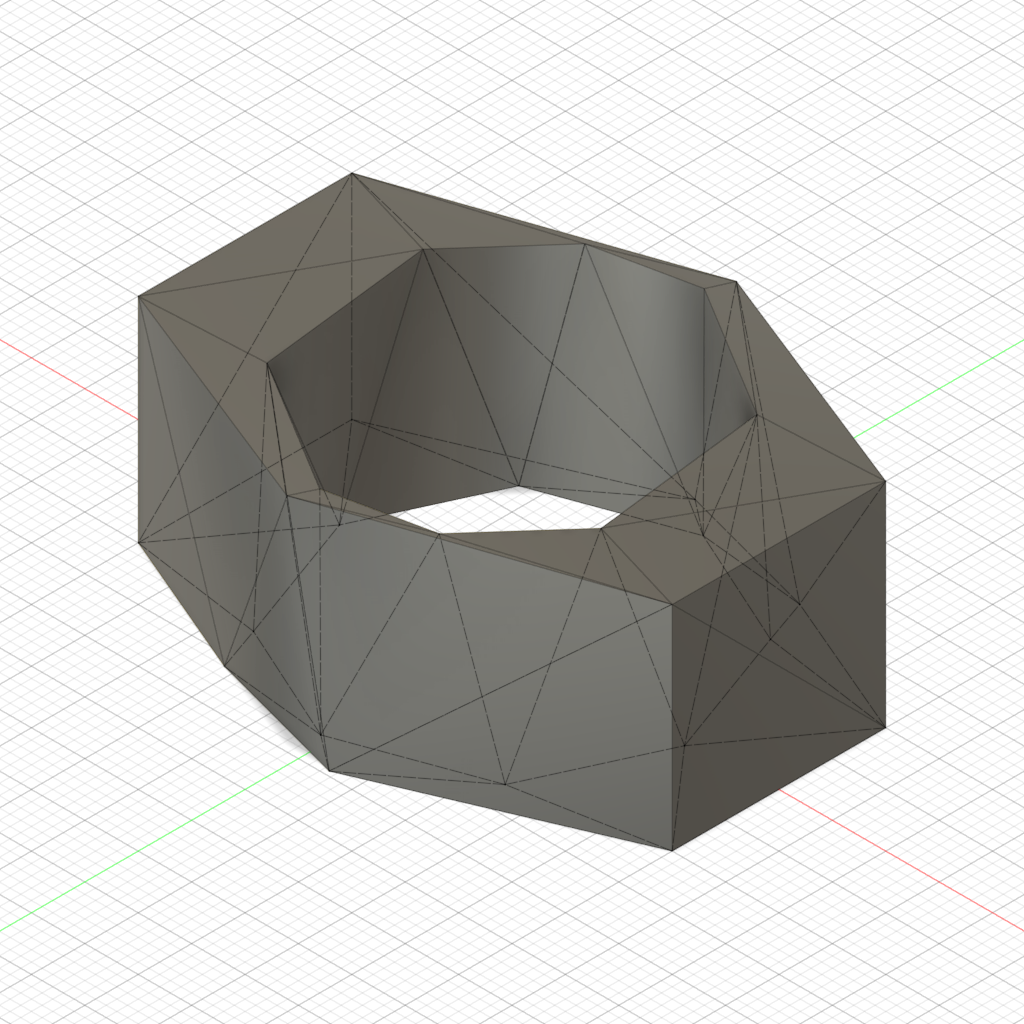
\includegraphics[width=\linewidth]{images/image_demo_low.PNG} % first figure itself
        \caption*{(c)}
    \end{minipage}\hfill

    \caption{Genauigkeit einer 3D-Datei ist abhängig von der Anzahl der gespeicherten
    Eckpunkte am Beispiel des Demonstratorbauteils. (a) 1512 Punkte
    (b) 52 Punkte (c) 30 Punkte}
    \label{fig:3d_design}
\end{figure}

\subsection{Scanner und Datenerfassung}
[todo verschiedene Scanner differenzieren und vergleichen]

Wie schon beschrieben, können dreidimensionale Daten direkt mit einem 
Scanner aufgenommen werden. 
Der Scanner hat, abhängig vom Modell und der angebrachten Höhe einen limitierten
Bereich, den er erfassen kann. 
Je nach Scannertyp und Modell kann sich der Messbereich ändern.
In Abbildung \ref{fig:scanner} ist ein Messbereich für den Scanner vom Typ 
ScanControl-LLT30xx sichtbar. Mittig kann 
in einer Tiefe von 85 mm eine Linie mit der Länge 25 mm gemessen werden. 
Der komplette messbare Bereich ist rot markiert. \cite{MESSTECHNIK_2020}
Bauteile die breiter sind als die maximale Breite der Scanebene, in Abbildung 
\ref{fig:scanner} mittig 25 mm, können also nicht in einer Pointcloud erfasst werden. 
Damit eine Digitalisierung von größeren Objekten erfolgen kann, müssen
also mehrere Scans durchgeführt, und später zusammengefügt werden. Zwischen den 
Scanvorgängen muss der Scanner in Richtung der Breitenachse verschoben werden.
Die Länge der Verschiebung sollte kleiner als die Scannerbreite sein, 
damit eine Überlappung entsteht, die 
genutzt werden kann, um die Pointclouds wieder zusammenzufügen. Die Verschiebung kann 
beliebig klein gewählt werden, jedoch steigt der Arbeitsaufwand und die Dateigröße mit 
jeder zusätzlichen Pointcloud, während das Ergebnis sich nicht verbessert.
Das Ergebnis verbessert sich nicht, da nicht mehr Daten aufgenommen werden, sondern nur 
die gleichen Daten mehrfach.
So können Pointclouds aufgenommen werden die dann in dem zu entwickelnde Verfahren
wieder zu einem digitalen Abbild zusammengefügt werden.

\begin{figure}[h]
    \centering
    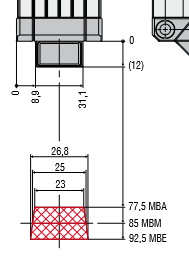
\includegraphics[width=0.3\textwidth]{images/Scanner.PNG}
    \caption{Funktionsweise eines Laserscanners [todo was ist abgebildet]}
    \label{fig:scanner}
\end{figure}

\section{Transformationen} \label{Transformation}

Eine Transformation ist eine Funktion, die eine Menge von Punkten in einem
Raum auf eine andere Menge von Punkten in demselben oder einem anderen Raum abbildet. 
Diese Transformationen werden verwendet, um die Lage, Form oder Größe von 
Objekten zu verändern.
Es gibt drei Basis Arten der Transformationen:
Translation, Rotation und Skalierung. Die Translation verschiebt alle Punkte 
um einen bestimmten Vektor in eine bestimmte Richtung. 
Rotation: Drehen eines Objekts um einen Punkt (in 2D) oder eine Achse (in 3D).
Veränderung der Größe eines Objekts durch Multiplikation der Koordinaten 
mit einem Skalierungsfaktor~\cite{XiaoleiDu.2009}.

\section{ICP-Algorithmus} \label{icp}

Der Iterative-Closest-Point-Algorithmus (ICP-Algorithmus) existiert schon seit dem Beginn der 90er Jahre und ist 
die klassische Methode, wenn es um die Registrierung von Pointclouds und 
anderen Punkt-Sets geht. \cite{icp}
Der Algorithmus errechnet eine lokale, optimale Transformation, die ein Daten-Set
dem anderen annähern kann. \cite{icp_og}
Um diese Transformation, zu bestimmen werden zuerst die Distanzen von allen 
Punkten in Daten-Set A zu dem jeweils nächsten Punkt in Daten-Set B aufsummiert 
werden. Dann wird eins der Daten-Sets verschoben und rotiert und wieder die 
Distanzen gebildet. Dies wird so lange gemacht bis die Änderung der Distanzen 
konvergiert. Die entstehende Transformation ist dann optimal.
Für identische Daten-Sets die sich nur in einer Transformation und Rotation 
unterscheiden, funktioniert dieser Algorithmus sehr gut. Bei Daten-Sets die 
Messfehler oder Überlappungen beinhalten kann häufig keine optimale 
Transformation bestimmt werden.
Deswegen wurden seit der ersten Vorstellung des Algorithmus viele Varianzen
entwickelt, die mit diesem Schwächen umgehen. 
Zum Beispiel der 'Sparse Iterative Closest Point' Algorithmus von~\cite{Bouaziz.2013}
oder die 'Anderson-accelerated' Version die besser mit Ausreißern und nur 
partiell überlappenden Daten umgehen kann und eine gleichwertige oder bessere 
Transformation errechnen kann.\ \cite{icp}
Der Algorithmus geht iterativ vor und berechnet immer eine optimale lokale Transformation.
Die beiden Daten-Set sollten schon vor dem Anwenden des ICP-Algorithmus grob angenähert sein, 
das beschleunigt die Konvergenz und damit die Laufzeit des Algorithmus.
Eine grobe Annäherung kann ermittelt werden, indem die Massenmittelpunkte der beiden Daten-Set
übereinander gelegt werden. In Abbildung \ref{fig:ipc_princip} ist das Prinzip visuell 
dargestellt. Die grünen Linien sind jeweils die kürzeste Distanz von Q nach R. 

\begin{figure}[h]
    \centering
    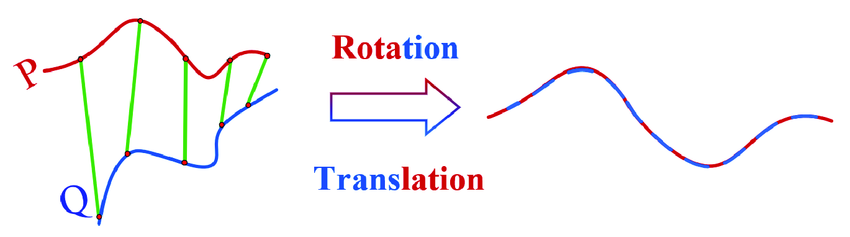
\includegraphics[width=0.7\textwidth]{images/Principle-of-ICP-algorithm.png}
    \caption{Prinzip des ICP-Algorithmus}
    \label{fig:ipc_princip}
\end{figure}




\chapter{Ziel der Arbeit}

Wie schon beschrieben müssen additiv gefertigte Bauteile nachbearbeitet werden
bevor sie eingesetzt werden können. 
Um eine korrekte Nachbearbeitung gewährleisten zu können muss das additiv 
gefertigte Bauteil fixiert werden. 
Dies kann vorgenommen werden, indem das Bauteil in einen Schraubstock eingespannt wird.

\section{Einspannproblematik}

Durch das Einspannen kann das Bauteil so deformiert werden, dass die vorgesehene Nutzung nicht mehr möglich ist. 
Je nach verwendetem Werkstoff und Geometrie kann die Deformation unterschiedlich
ausfallen. 

\section{Erfassung der spannkraftinduzierten Deformation}

Für die Beurteilung, ob ein Bauteil noch eingesetzt werden kann, ist es nötig die 
Deformation die auf das Objekt gewirkt hat zu erkennen. Wenn das Bauteil in einen 
Schraubstock eingespannt wird, wirkt eine Spannkraft über die Backen des Schraubstock
auf das eingespannte Bauteil. 
Diese Kraft induziert eine Deformation auf das Bauteil. Diese Deformation soll 
optisch in einem Verfahren erkannt und dargestellt werden.

\section{Verfahren zur optische Spannkraftdeformationserkennung}

Um die Deformation des Bauteils erfassen zu können wird das 3D-Objekt benötigt, 
dass als Grundlage für die AF diente. Zusätzlich werden optische Daten des Bauteils 
im deformiertem Zustand benötigt. Mit diesen beiden Daten kann der Unterschied 
ermittelt und ausgegeben werden.
Um auch minimale Deformationen erkennen zu können müssen die Daten des 
eingespannten Bauteils hinreichend genau sein. Deswegen wird ein Laserscanner zur 
Datenerfassung eingesetzt.
Wie schon beschrieben ist der Messbereich eines Laserscanners begrenzt. Da das 
Verfahren nicht auf eine Bauteilgröße beschränkt sein soll, müssen mehrere Scans als 
Eingabe akzeptiert und damit umgegangen werden.

\section{Vorgehen}

Das Verfahren, um eine Deformation in einem eingespannten additiv gefertigten
Bauteil, zu erkennen umfasst folgenden Schritte:

\begin{itemize}
    \item \textbf{Digitalisierung des Bauteils:}\\
        In diesem Schritt werden Messfehler und Ausreißer
        in den Scannerdaten entfernt. Anschließend werden die dreidimensionalen 
        Eingangsdaten in eine zweidimensionale Ansicht umgewandelt.
        Nach diesem Schritt liegen für jedes Bauteil mehrere Datensätze als 
        zweidimensionale schwarz weiß Bilder vor.
    \item \textbf{Stitching Methodik}\\
        Diese Bilder müssen nun zu einem einzelnen Bild zusammengefügt werden.
        Hierfür werden Gemeinsamkeiten in den sich 
        teilweise überlappenden Bildern gesucht und eine Transformation ermittelt,
        die auf eines von zwei Bildern angewendet werden kann, um sie zusammenzufügen.
    \item \textbf{Deformationserkennung}\\
        Sobald ein Bild für ein eingespanntes Bauteil vorliegt, können verschiedene 
        Zustände des Bauteils verglichen werden. Deformationen werden erkannt, in dem 
        die Länge und Breite des Bauteils verglichen wird, zusätzlich wird der 
        Abstand zwischen den Rändern des Bauteils berechnet. Es können verschiedene
        Spannungszustände verglichen werden, ein Vergleich mit dem initialen 
        3D-Design ist auch möglich. Hier werden auch Fehler erkannt die im 
        Fertigungsprozess entstehen erkannt. Der Unterschied zwischen Bauteilzuständen
        wird auch visuell ausgegeben und als Bild gespeichert.
        
\end{itemize}



























\chapter{Datenaufbereitung} \label{prepareData}

Um die Deformation im eingespannten Zustand zu erkennen, muss das komplette Werkstück
als digitales Modell existieren, um es mit anderen Modellen vergleichen zu können.
Das hier zu entwickelnde Verfahren soll die Deformation nur in einer zweidimensionalen Perspektive erkennen. 
Das ist weniger komplex, hat aber zur Folge, dass Bauteile mit unterschiedlichen 
Oberflächenhöhen nicht vollständig analysiert werden können. 
Geometrie und Oberflächeninformationen des eingespannten Bauteils liegen 
in Form von mehreren Pointclouds vor.
Diese Daten wurden mithilfe eines Laser-Profilsensors aufgenommen 
(siehe Kapitel \ref{lasers}). Durch diesen Prozess 
entstehen Messfehler und Ausreißer. Diese Punkte verfälschen das Verfahren da sie 
nicht auf dem eingespannte Bauteil liegen. Die Genauigkeit des Verfahrens profitiert, 
wenn diese Punkte entfernt werden. Ausreißer sind in Abbildung \ref{fig:pcs} (a) 
zu sehen.

\section{Pointcloud filtern}
    
Ausreißer können aus Pointclouds entfernt werden, indem einzelne Punkte 
relativ zu ihren Nachbarpunkten im dreidimensionalen Raum betrachtet werden.
Zur Erkennung und Entfernung von Ausreißern sind in der Open-Source
Bibliothek 'Open3D' zwei Methoden vorhanden. 
Die Methode \glqq radius\_outlier\_removal\grqq~entfernt Ausreißer basierend auf 
einem konfigurierbaren Radius. Punkte die weniger als n andere Punkte in dem Radius 
haben werden entfernt. Die andere Methode lautet 
\glqq statistical\_outlier\_removal\grqq~ 
und entfernt alle Punkte, die weiter von ihren Nachbarn entfernt sind, als die 
statistische Varianz aller Entfernungen. \cite{Zhou.30012018}

Die erste Methode eignet sich gut, wenn die Maße des Objekts bekannt
sind. Dann kann der Radius entsprechend der Größenordnung des Bauteils gewählt werden.
Da das hier zu entwickelnde Verfahren sich nicht auf eine Bauteilgeometrie 
beschränken soll, ist dieses Verfahren nicht geeignet. 
Durch eine Annahme des Radius würden ein Bias 
zu kleinen oder großen Bauteile entstehen.
Stattdessen wird die statistische Herangehensweise genutzt. 
Hier werden Punkte gelöscht, die weiter von ihren benachbarten Punkten entfernt
sind als der durchschnittliche Abstand der Punkte in der gesamten Pointcloud. 
Umso mehr benachbarte Punkte betrachtet werden, desto länger dauert der Filterprozess.

Beim Filtern werden zwischen sieben und zehn Prozent der Punkt in der Pointcloud entfernt.
In Abbildung~\ref{fig:pcs} sind Pointclouds vor und nach dem Entfernen von Ausreißern 
dargestellt.

\begin{figure}[H]
    \centering
    \begin{minipage}{0.45\textwidth}
        \centering
        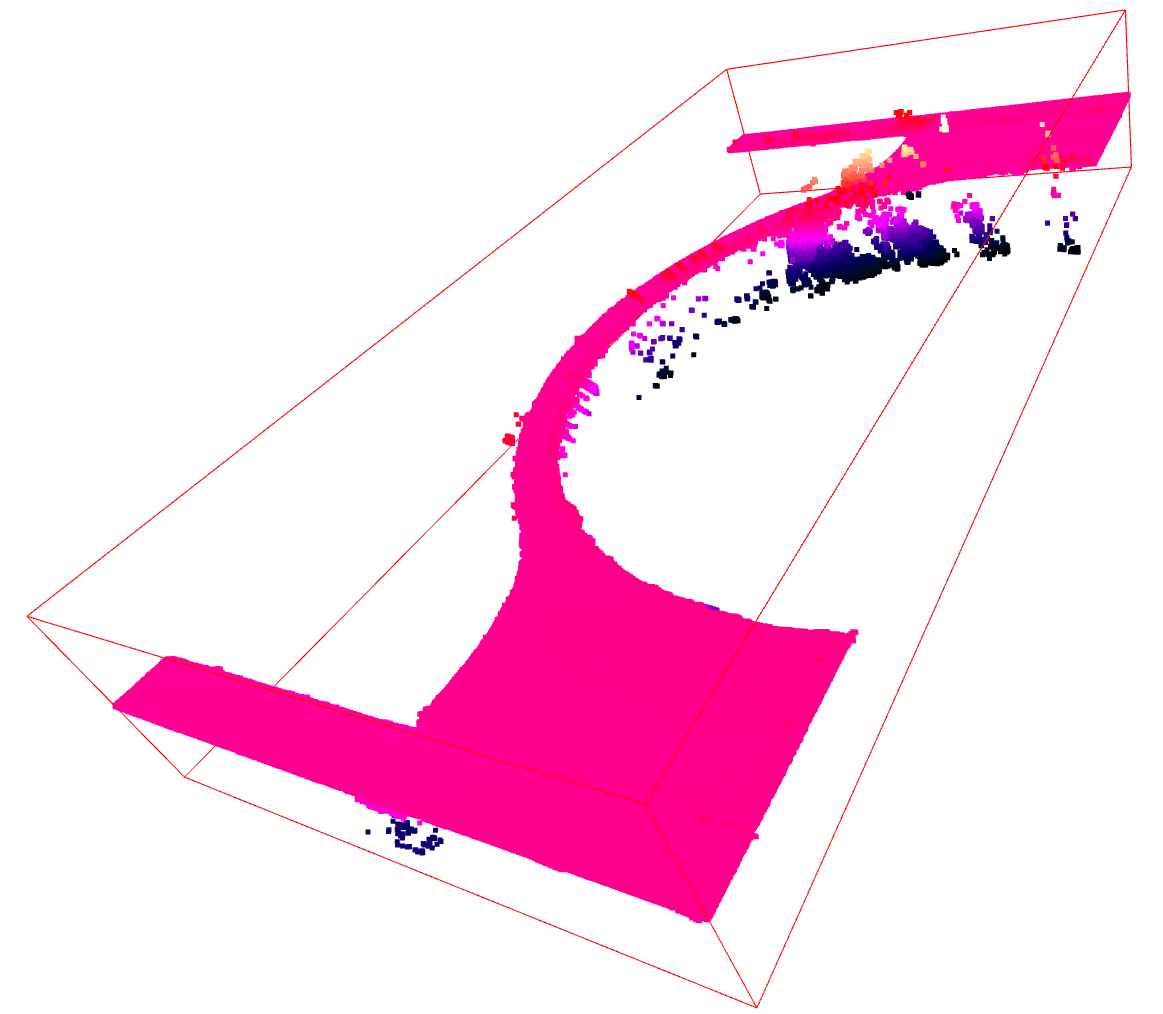
\includegraphics[width=\textwidth]{images/pc_with_outliers.PNG} % first figure itself
        \caption*{(a)}
    \end{minipage}\hfill
    \begin{minipage}{0.45\textwidth}
        \centering
        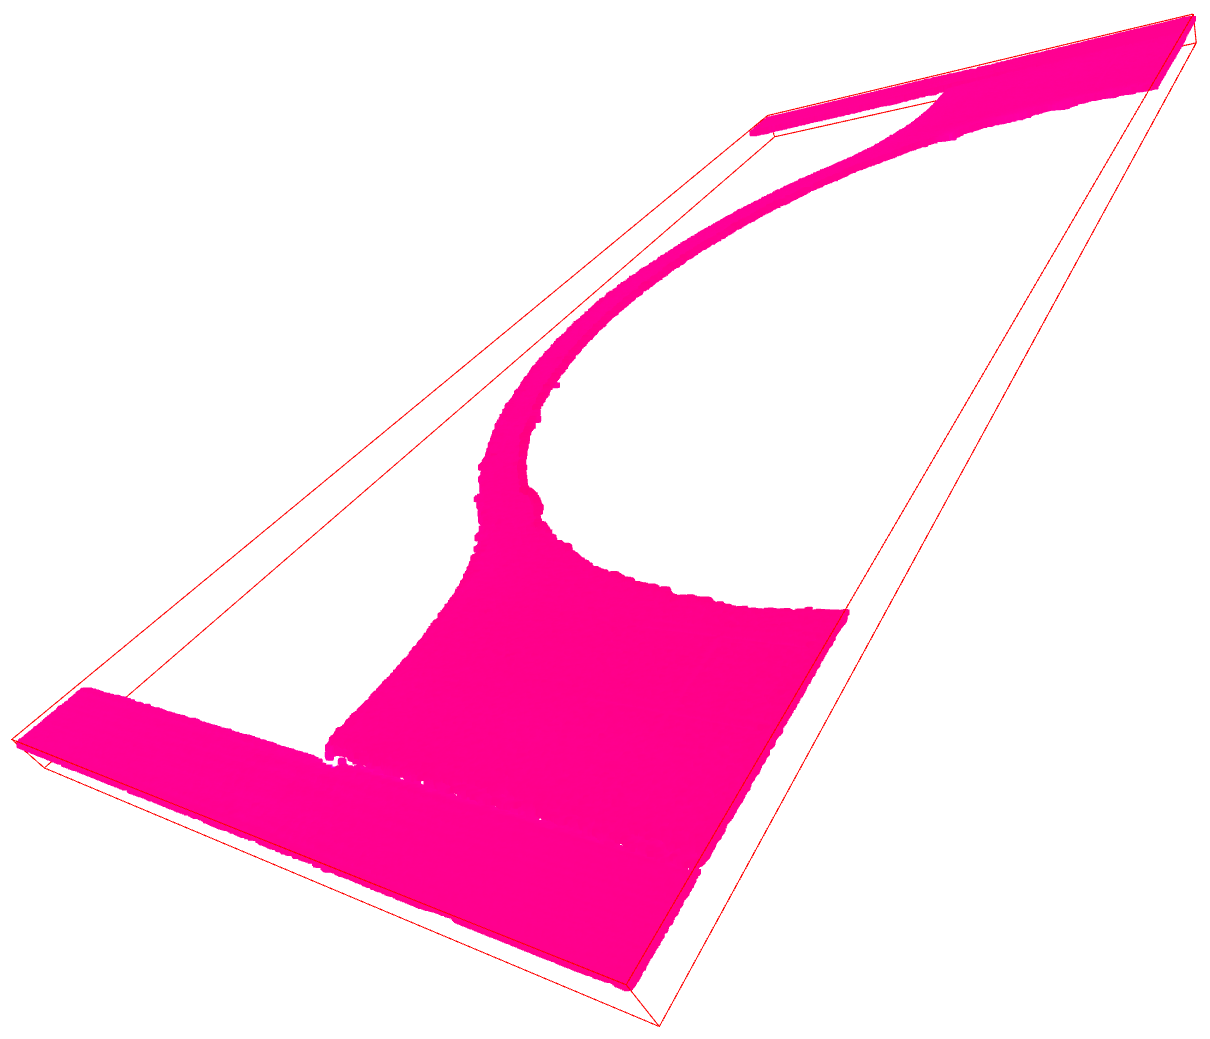
\includegraphics[width=\textwidth]{images/pc_without_outliers.PNG} % second figure itself
        \caption*{(b)}
    \end{minipage}
    \caption{Pointcloud eines Metallbauteils, in (a) ohne Filterung,
    in (b) mit den Ausreißern entfernt.}
    \label{fig:pcs}
\end{figure}

\section{Pointcloud in Bild konvertieren}

Um Rechenzeit zu sparen und die zahlreichen Funktionen bereits bestehender
Bilderkennungsbibliotheken nutzen zu können, werden die Pointclouds in Bilder 
konvertiert. Hierfür wird zunächst ein leeres Bild mit den gleichen 
Maßen der Pointcloud erstellt. Anschließend wird über alle Punkte der
Pointcloud iteriert und der Pixel an den 
entsprechenden X- und Y-Koordinaten des Punktes auf einen Helligkeitswert gesetzt.

Um Rechenzeit und Speicherkapazitäten zu schonen und 
da es für die Berechnungen ausreichend ist, wurden 
8-Bit-Single-Channel-Bilder verwendet, die nur Helligkeitswerte abbilden und keine 
Farbinformationen.
In diesen Bildern kann jeder Pixel einen Wert zwischen 0 und 255 annehmen. 
Der entsprechende Helligkeitswert wird wie folgt berechnet:
\begin{align*}\label{calc:brightness}
    value_p = \frac{Z - min_z}{max_z - min_z} \cdot (max_{brightness} - min_{brightness}) + min_{brightness}
\end{align*}
Der resultierende Wert ist die Helligkeit, die dem Pixel zugewiesen wird.
$Z$ ist die Z-Koordinate des Punktes in der Pointcloud. $min_y$ und $max_y$ sind 
die Grenzen der Z-Koordinate, diese werden gebraucht um die Helligkeit relativ 
zu der Höhe zu berechnen. $min_{brightness}$ und $max_{brightness}$ sind die gewünschten Grenzen der 
Helligkeit. In unserem Fall sind $min_{brightness} = 0$ und $max_{brightness} = 255$ da ein acht Bit Bild
verwendet wird.

In Abbildung \ref{fig:image_from_pc} ist das resultierende Bild eines Scans von einem 
FDM Bauteil zu sehen. Es fällt auf, dass kaum Helligkeitsveränderungen
im Bild sichtbar sind. Das liegt an derselben Problematik, an der der ICP-Algorithmus
 (vgl. Kapitel \ref{icp}) häufig
scheitert. Reale Datensets spiegeln die Realität nicht ganzheitlich korrekt wider, 
sondern beinhalten Messfehler und Streuungen, die trotz der Filterung der Pointcloud
bestehen bleiben.

\begin{figure}[H]
    \centering
    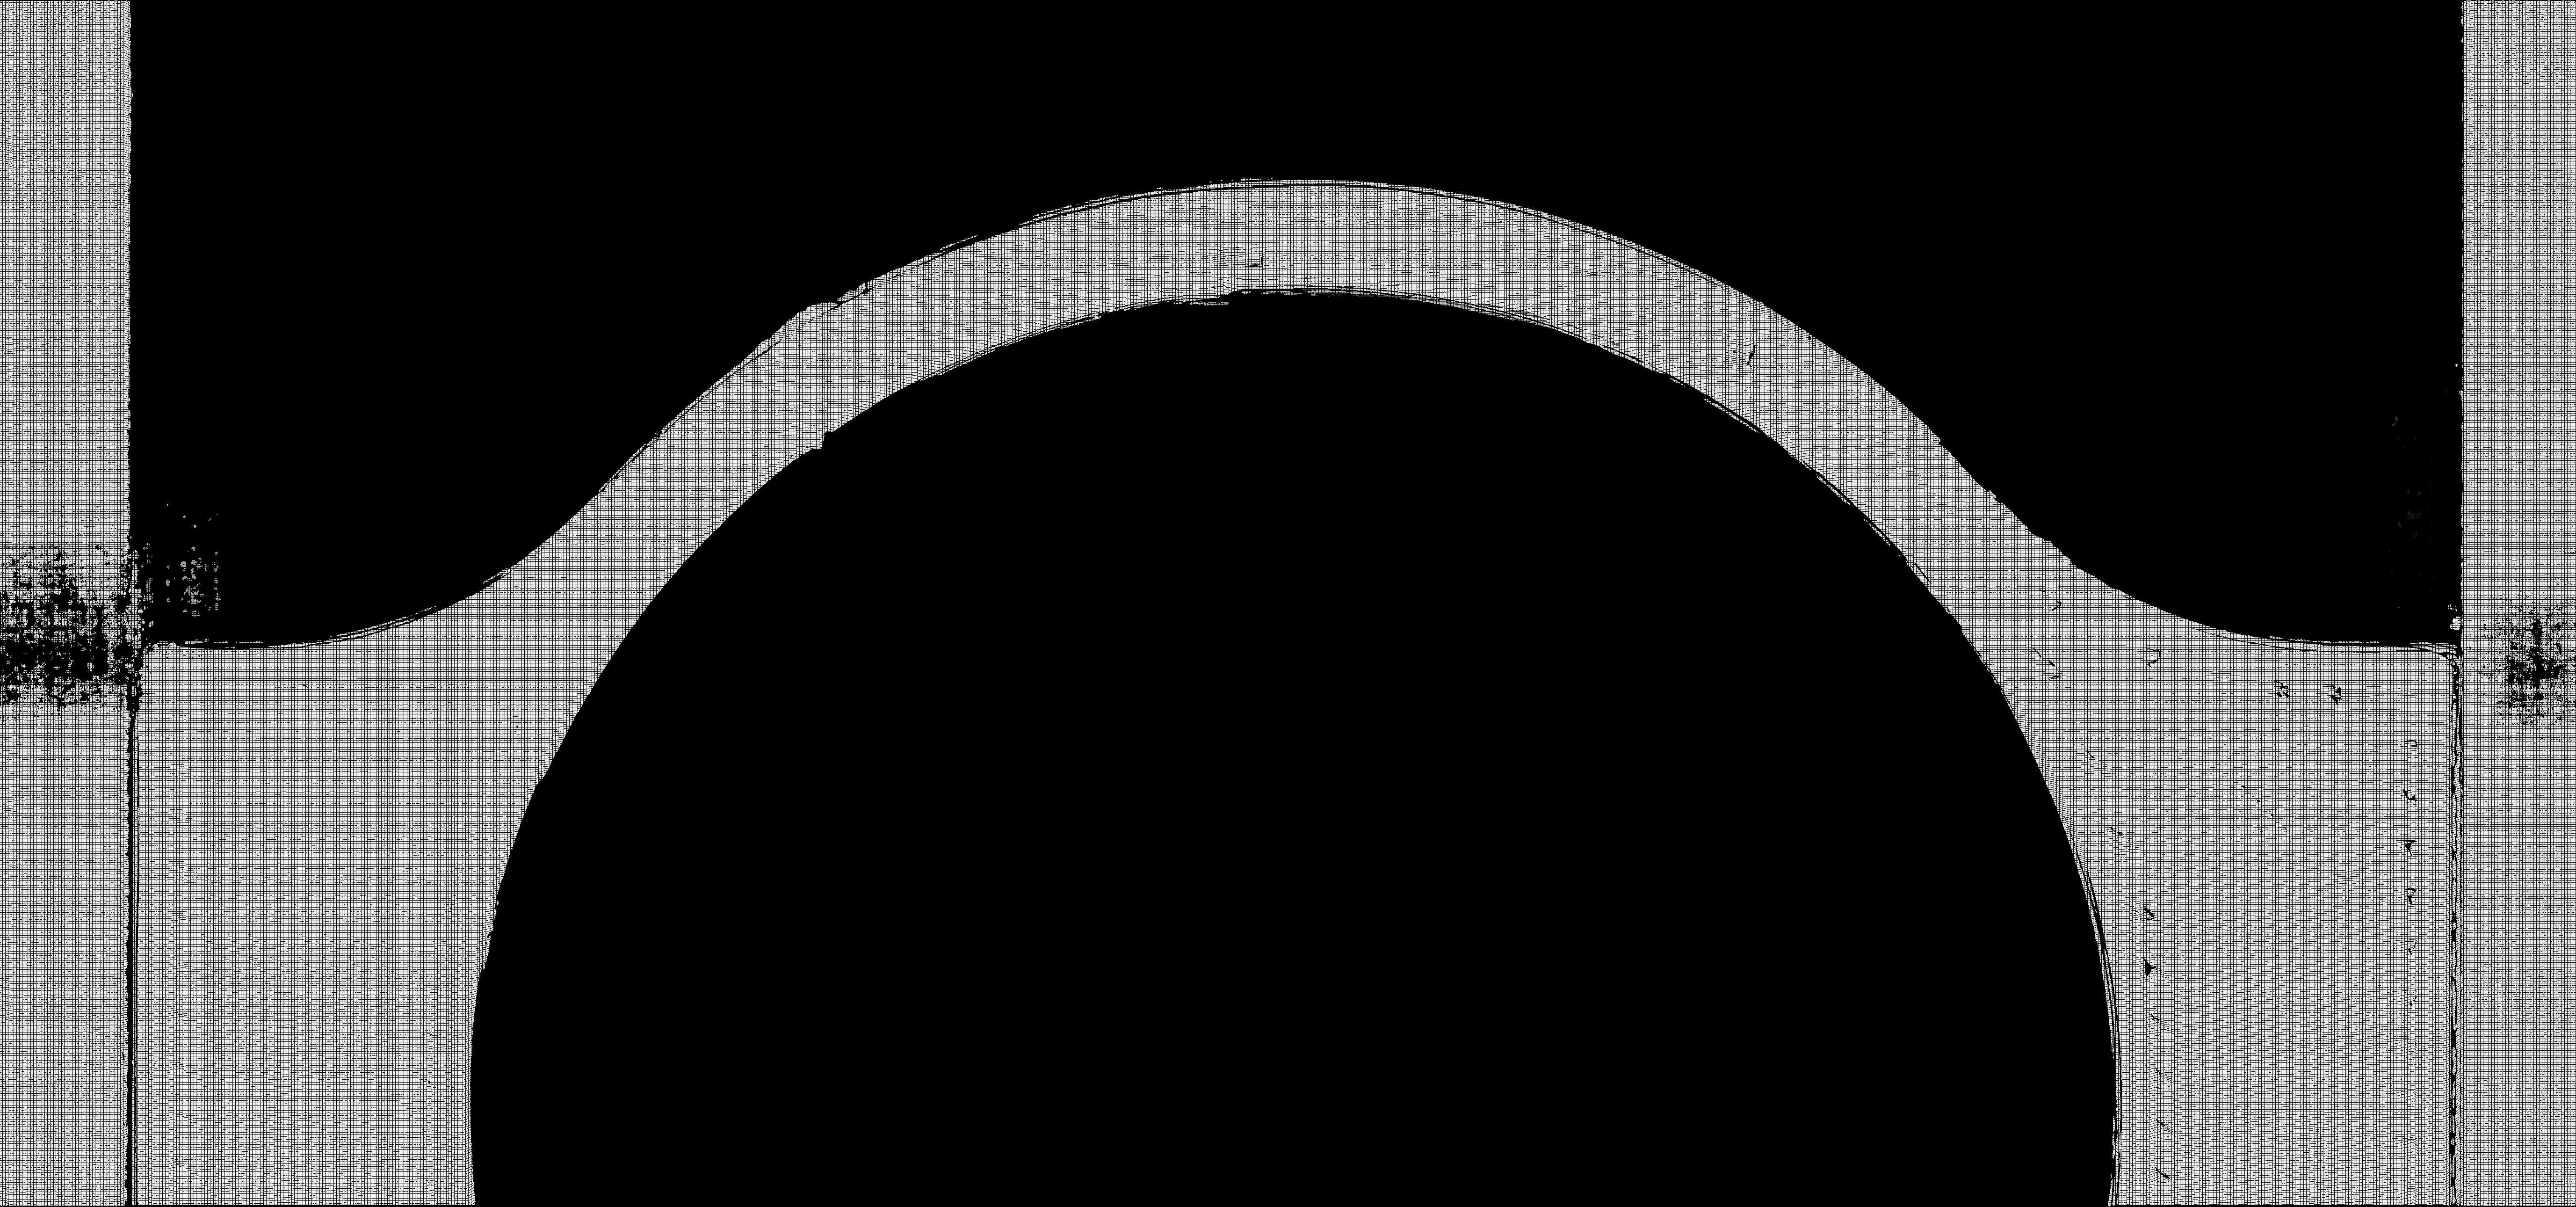
\includegraphics[width=0.9\textwidth]{images/fdm_top_100p.png}
    \caption{Resultat der Pointcloud zu Bild Konvertierung eines FDM Bauteils, 
    ohne zusätzliche Filterung der Höheninformationen.}
    \label{fig:image_from_pc}
\end{figure}

Damit das resultierende Bild die Höheninformationen besser widerspiegelt, werden 
die Scandaten erneut gefiltert. In diesem Filterprozess werden die Daten nicht, 
wie zuvor, im dreidimensionalen Raum betrachtet, sondern es werden ausschließlich 
die Höheninformationen der Pointcloud betrachtet.

Abbildung \ref*{fig:brightness} zeigt die Häufigkeitsverteilung der Höhenwerte einer
Pointcloud von dem Demonstratorbauteil (siehe Kapitel \ref{demo_Bauteil}). 
In blau ist die Verteilung der Punkte auf 
einem Demonstratorbauteil zu sehen, das aus Metall gedruckt wurde, orange zeigt die 
Verteilung der Punkte auf einem Kunststoffteil.
In dem oberen Histogramm 
sind die Häufigkeiten der Höhenwerte zu sehen. Der Datensatz wurde in 1000 gleich große
Teile gruppiert, jeder Balken repräsentiert eine Gruppe.
In \ref*{fig:brightness} (b) ist das Histogramm mit dem gleichen Datensatz wie in (a) 
dargestellt, aber mit der y-Achse 
logarithmisch skaliert um kleine Prozente deutlich zu machen die in Diagramm
(a) nur schwer oder gar nicht sichtbar sind. 
Die meisten Höhenwerte treten bei ca. 80 mm beziehungsweise 85 mm auf, 
sie gehören zu den Punkten, die auf dem Demonstratorbauteil liegen, 
es treten allerdings auch Werte darunter und darüber auf. 
Die in \ref*{calc:brightness} vorgestellte Formel benutzt allerdings 
die absoluten Minimum und Maximum Werte.
Alle Punkte die tatsächlich auf dem Bauteil werden also entsprechend wenig
berücksichtigt. Dies kann verhindert werden, indem Werte, die weniger häufig 
auftreten, entfernt werden.

\begin{figure}[H]
    \centering
    \begin{minipage}{\textwidth}
        \centering
        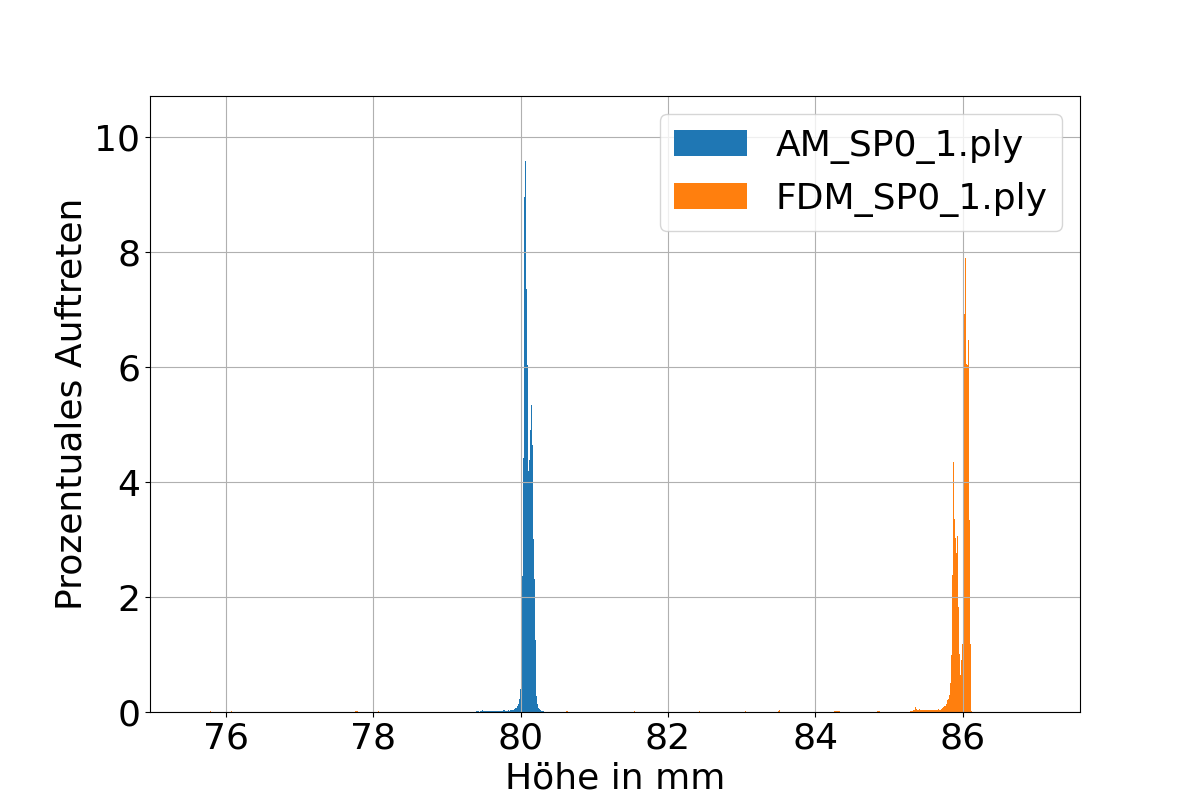
\includegraphics[width=0.8\textwidth]{images/height_occurange.png} % first figure itself
        \caption*{(a)}
    \end{minipage}\hfill
    \begin{minipage}{\textwidth}
        \centering
        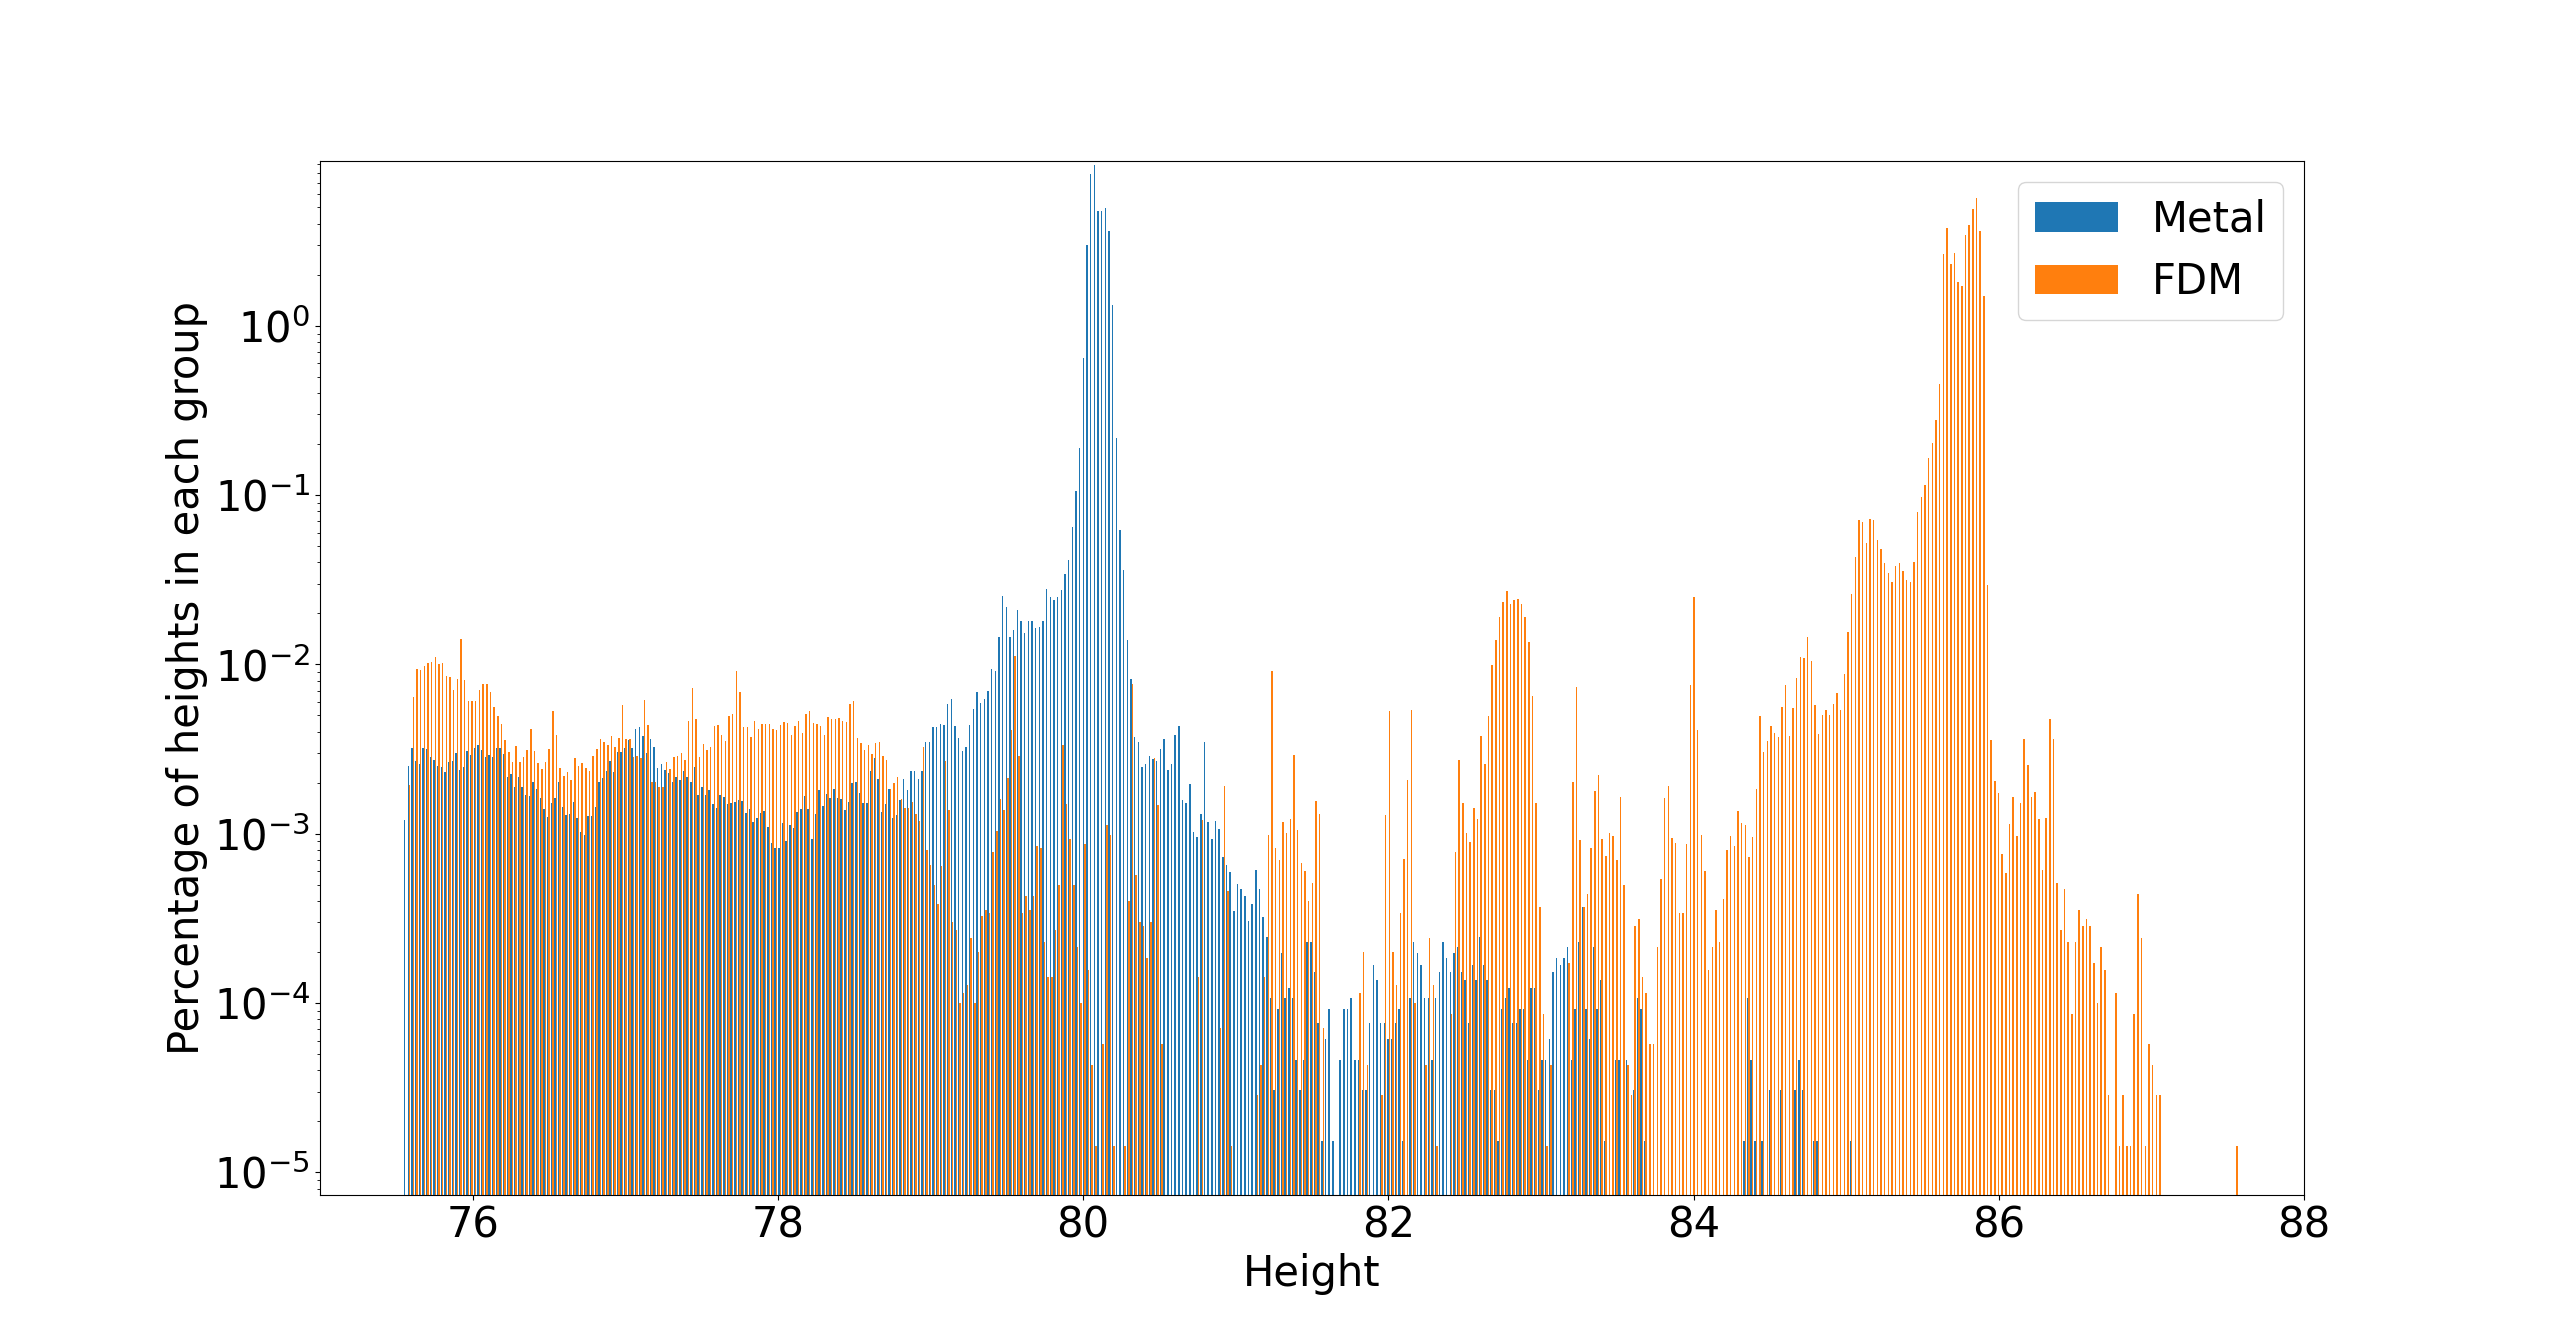
\includegraphics[width=0.8\textwidth]{images/height_occurange_log.png} % second figure itself
        \caption*{(b)}
    \end{minipage}
    \caption{Auftreten der Höhenwerte in den Scandaten der Demonstratorbauteile. 
    (a): Das Histogramm ist nicht skaliert. (b): Logarithmische Skalierung der 
    Höheninformationen. Hier ist zu sehen, dass die Höhenhäufigkeiten streuen.}
    \label{fig:brightness}
\end{figure}

Werden alle Höhenwerte nach der Häufigkeit ihres 
Auftretens in der Pointcloud sortiert, und der n-ten Prozentsatz entfernt, können
zusätzliche Ausreißer entfernt werden.
Ränder und Oberflächenstrukturen auf dem Bauteil können dadurch deutlich besser erkannt werden. 
Dadurch sind auch die Markierungen auf der linken und rechten Seite sichtbar geworden,
diese sollen bei der Registrierung
helfen. Zusätzlich sind die Spuren und Lücken die durch den FDM 
Herstellungsprozess entstehen zu sehen.
Durch das Filtern der Höheninformationen sind Oberflächenstrukturen nicht nur besser
erkennbar, auch die Ränder treten genauer hervor. 
Dadurch können die Bilder im weiteren Schritt korrekt zusammengefügt werden.
In Abbildung \ref{fig:10p} ist das resultieren Bild zu sehen, wenn nur die zehn Prozent
häufigsten Höhenwerte verwendet werden.
Die Spuren des FDM Fertigungsprozess sind deutlich zu sehen.

\begin{figure}[H]
    \centering
    \includegraphics[width=0.95\textwidth]{images/fdm_top_10p.png}
    \caption{Resultat der Pointcloud zu Bild Konvertierung eines FDM Bauteils.}
    \label{fig:10p}
\end{figure}


\chapter{Stitching}

Für jeden Einspannzustand eines Bauteils können mehrere Bilddateien vorliegen.
Alle Bilddateien gehören zu dem gleichen Bauteil und müssen 
zusammengefügt werden, um ein einzelnes Bild zu erhalten. 
Als Voraussetzung ist gegeben, dass alle Bilder Überlappungen enthalten.

Diese Überlappung kann benutzt werden, um die Bilder zu einem Bild zusammenzufügen.
Für das Stitching von Bilddateien existieren schon mehrere Verfahren, die in Bibliotheken
für viele Programmiersprachen implementiert sind. Der schon beschriebene 
ICP-Algorithmus \ref{icp}
ist eines dieser Verfahren. Das Problem mit diesen Verfahren ist, dass zwei 
Datensätze registriert werden, indem auf ein Datensatz so lange eine 
Transformation (vgl. \ref*{Transformation}) angewendet wird, bis
die Distanz der Datensätze unter einen Grenzwert fällt oder nicht mehr verbessert
werden kann. Die Überlappung in den von dem Laserscanner aufgenommen Daten ist jedoch 
nur in zwei Achsen verschoben. Durch eine Rotation kann eine Transformation 
berechnet werden, die nicht der Realität entspricht, gesucht ist eine Transformation 
die ausschließlich aus einer Translation in zwei Achsen besteht.

Um die korrekte Transformation zu finden, mit der die beiden Bilder überlappen,
muss nicht der komplette Bereich analysiert werden, sondern nur der überlappende Teil.

In diesem Bildausschnitt müssen gemeinsame Bereiche in beiden Bildern erkannt werden. 
Diese gemeinsamen Bereiche können anschließend miteinander verglichen werden.
Bereiche, die verglichen werden können, sind Ränder oder Farbunterschiede im Bild 
und werden im folgenden als Features bezeichnet.

\section{Feature Erkennung} \label{contoursearching}

Features in einem Bild sind große Unterschiede in benachbarten Pixeln. Die größten
Features sind die Ränder des Bauteils, kleinere Features können Oberflächenänderungen 
oder Spuren des Herstellungsprozesses sein. Diese Unterschiede können mithilfe 
der 'OpenCV' Bibliothek extrahiert werden. Diese Bibliothek gibt die erkannten 
Features als Liste von Konturen aus. Konturen selbst bestehen aus Listen von 
Punkten, die aus X und Y Koordinaten bestehen. Die Konturerkennung kann verbessert 
werden, indem das Bild entsprechend präpariert wird. In Abbildung \ref{fig:cons} und
\ref{fig:image_top} ist ein Ursprungsbild und die extrahierten Konturen zu sehen.
Mittig am linken und rechten Rand sind in Abbildung~\ref{fig:cons}
Messfehler des Laserscanners zu sehen. Diese werden auch als Features in 
Abbildung \ref{fig:image_top} erkannt. Diese müssen entfernt werden, damit die Bilder 
korrekt zusammengefügt werden können. Erfolgt dies nicht werden diese Fehler miteinander
verglichen, was das Ergebnis verfälscht.

\begin{figure}[h]
    \centering
    \includegraphics[width=0.8\textwidth]{images/with_con.jpg} % first figure itself
    \caption{Oberes Bild eines Scanvorgangs, FDM Bauteil}
    \label{fig:image_top}
\end{figure}

\begin{figure}[h]
    \centering
    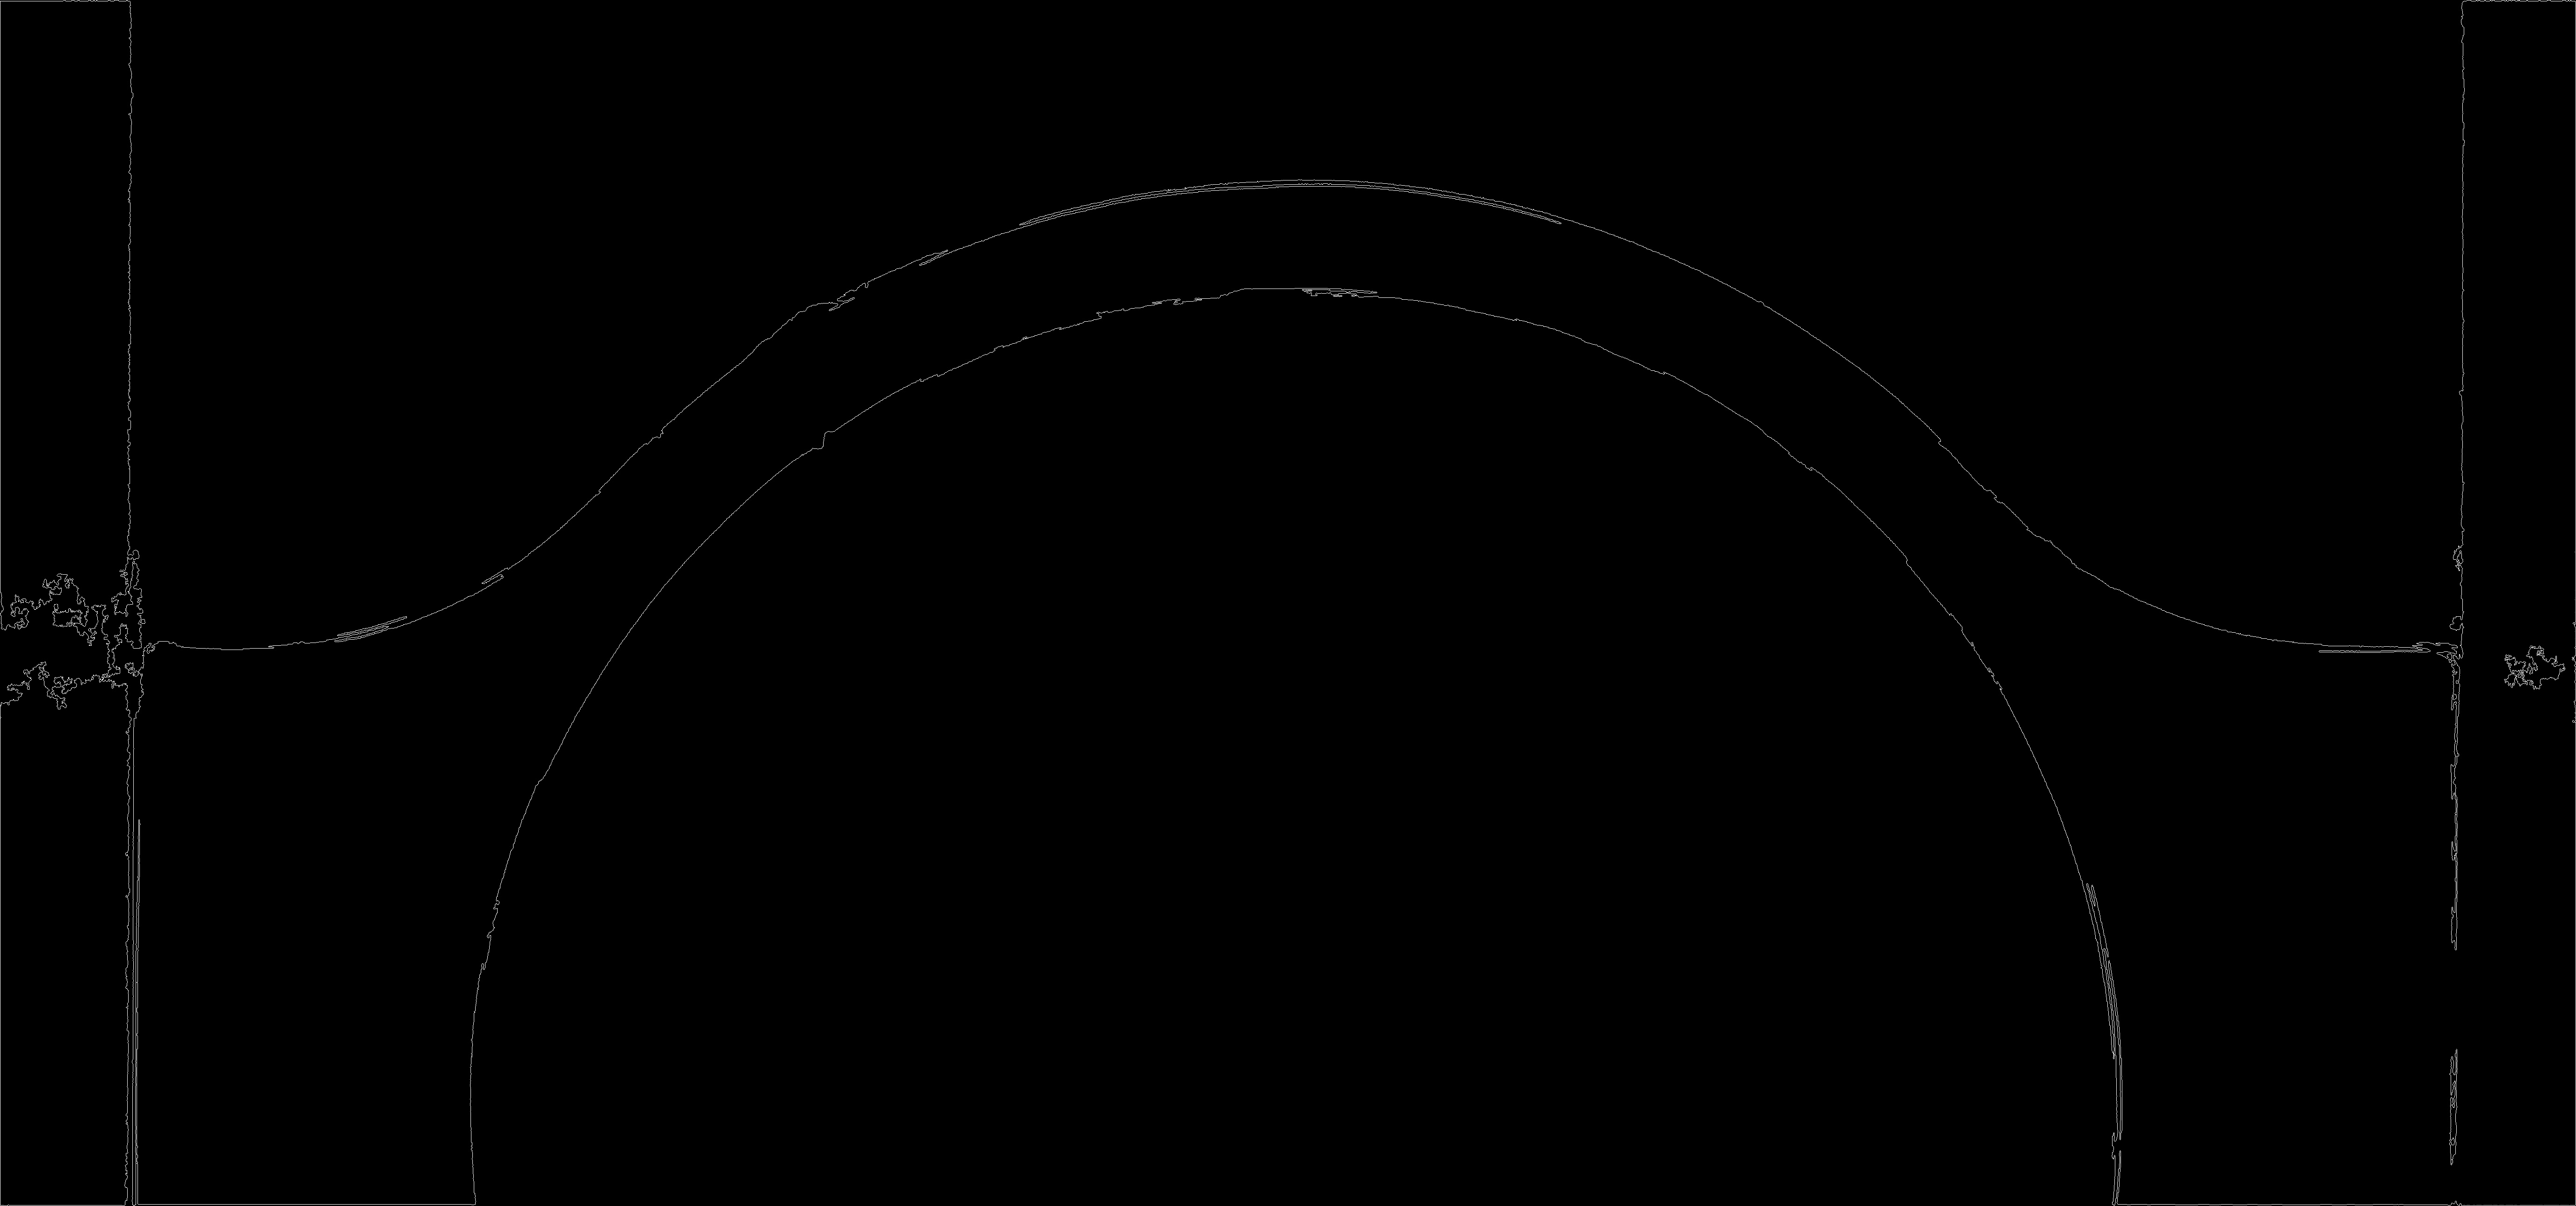
\includegraphics[width=0.8\textwidth]{images/only_con.jpg} % second figure itself
    \caption{Extrahierte Konturen des Bildes ohne Pre-Processing [TODO besseres Bild einfügen]}
    \label{fig:cons}
\end{figure}

Die Überlappung kann nur im oberen oder unteren Bildbereich auftreten. Der restliche 
Teil des Bildes kann also entfernt werden. So wird außerdem Rechenzeit gespart.

\begin{figure}[h]
    \centering
    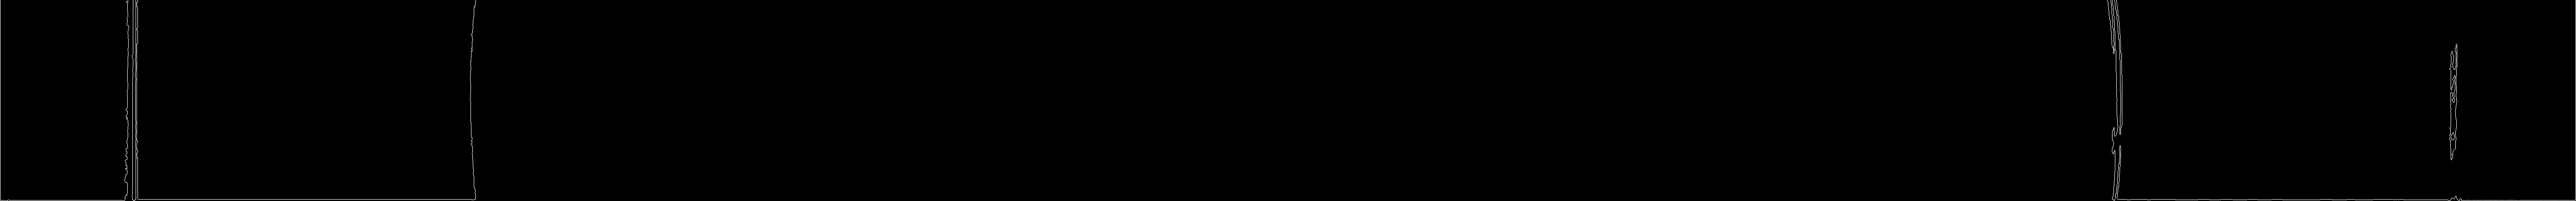
\includegraphics[width=0.8\textwidth]{images/only_con_cut.jpg} % second figure itself
    \caption{Extrahierte Konturen des Bildes ohne vorheriges filtern, zugeschnitten 
    auf den überlappenden Bereich [TODO besseres Bild einfügen]}
    \label{fig:cons_cut}
\end{figure}

Dieses Verfahren wird auf beide Bilder angewendet. Daraus resultieren dann zwei 
zugeschnittene Bilder aus denen Konturen extrahiert wurden. 
Würden diese beiden Bildteile vollständig überlappen, könnte jetzt der ICP-Algorithmus
angewendet werden. Dieser würde dann die korrekte Transformation berechnen, in dem er 
die Konturen aus dem oberen Bild, mit denen aus dem unteren Bild vergleicht und die 
Distanz zwischen den Punkten minimiert. 
Der Grad der Überlappung ist unbekannt und kann nicht im Vorhinein bestimmt werden.
Dadurch kann der ICP-Algorithmus nicht eingesetzt werden. 
Eine andere wichtige Annahme kann getroffen werden: Jeweils eine Kontur aus 
dem oberen und unteren Bild haben mindestens einen gemeinsamen Punkt.

\section{Differenzierung von Punkten}

Die Distanz zwischen zwei Punkten kann über den euklidischen Abstand gemessen werden.
\cite{Dokmanic.2015}. Sei A ein Punkt in einer Kontur aus dem oberen Bild und K eine 
Kontur aus dem unteren Bild.  
Um den Punkt aus K zu finden, der am nächsten an A liegt, muss A mit jedem Punkt aus 
K verglichen werden. Das Punktepaar mit dem kleinsten gefunden euklidischen Abstand 
wird als \glq Best Match\grq gespeichert. Wenn die euklidische Distanz null beträgt, kann 
die Suche abgebrochen werden, da kein kleinerer Wert mehr gefunden werden kann.
Dieser Ansatz ist dem ICP-Algorithmus ähnlich. Die Differenz zwischen zwei Konturen 
K1 und K2 kann verglichen werden, indem für jeden Punkt A aus K1 der näheste Punkt aus 
K2 gefunden wird. In dem ICP-Algorithmus werden alle Distanzen von der \glq Best Matches \grq 
aufsummiert und beschreiben den Unterschied der beiden Distanzen. Diese Summe kann dann 
minimiert werden. Dieser Ansatz funktioniert bei einem sich nur partiell
überlappenden Datensatz nicht. 
Statt die Summe zu bilden, wird jede beste Distanz zusammen mit ihren korrespondieren 
Punkten gespeichert. Um den Grad der Überlappung zu bestimmen, werden die Distanzen 
gezählt die gleich null sind. Dieser Wert in Relation zu der Länge von K1 gibt, 
in Prozent, an zu welchem Anteil sich die beiden Konturen überlappen.

\section{Transformation bestimmen}

Gesucht ist die Transformation welche die maximale Überlappung der beiden 
Konturen K1 und K2 bietet. Um diese Transformation zu berechnen, muss der 
Grad der Überlappung für jede mögliche Positionierung ermittelt werden. Jeder
Punkt aus K2 muss auf die Koordinaten eines beliebigen aber festen Punkts aus K1 
verschoben werden.
Die Transformation zwischen zwei Punkten A und B kann über die Vektorberechnung erfolgen:

\begin{equation*}
    T_{a,b} = \begin{pmatrix}a_x\\a_y\end{pmatrix} - \begin{pmatrix}b_x\\b_y\end{pmatrix}
\end{equation*}

Kontur K2 kann über Kontur K1 verschoben werden, indem Punkt A festgehalten wird, 
während Punkt B sukzessive jeden Punkt aus K2 annimmt. 
Die daraus resultierende Punkttransformation wird auf jeden Punkt von K1 angewendet, 
um die nächstgelegenen Nachbarpunkte zu ermitteln. Für jede Transformation wird der 
Überlappungsanteil berechnet, wobei das Ergebnis mit der maximalen Überlappung
als die optimale Transformation gespeichert wird.
Dieses Verfahren ist nur anwendbar, wenn Punkt A im überlappenden Bereich liegt. 
Befindet sich Punkt A nicht in der Kontur K2, 
kann das Verfahren nicht erfolgreich angewendet werden.
Zur Berechnung der optimalen Transformation werden verschiedene Punkte aus K1 
ausgewählt und das Verfahren jeweils angewendet. 
Die Transformation mit dem größten Verhältnis von Nullen zur
Gesamtlänge der Kontur wird als optimal angesehen. 
Aufgrund des exponentiellen Laufzeitverhaltens ist es ineffizient, 
jeden Punkt A aus K1 mit jedem Punkt B aus K2 zu vergleichen.

In Abbildung \ref{fig:k1_and_k2} (a) sind zwei Beispielkonturen zu sehen. 
Diese sind nicht angeordnet. Der ICP-Algorithmus würde diese beiden Konturen 
annähern, ohne sie zu überlappen. 
Das Ergebnis des vorgestellten Stitching Verfahrens ist in Abbildung 
\ref{fig:k1_and_k2} (b) zu sehen. Es ist zu erkennen das, trotz Messfehler und 
kleineren unterschieden im überlappenden Bereich die korrekte Transformation 
ermittelt werden konnte. Diese Konturen stammen von einem additiv gefertigten 
Metallbauteil.

\begin{figure}[h]
    \centering
    \begin{minipage}{0.49\textwidth}
        \centering
        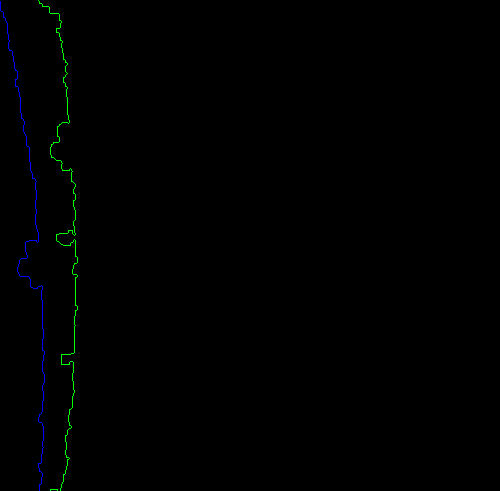
\includegraphics[width=\textwidth]{images/before_matching.png} % first figure itself
        \caption*{(a)} 
    \end{minipage}\hfill
    \begin{minipage}{0.49\textwidth}
        \centering
        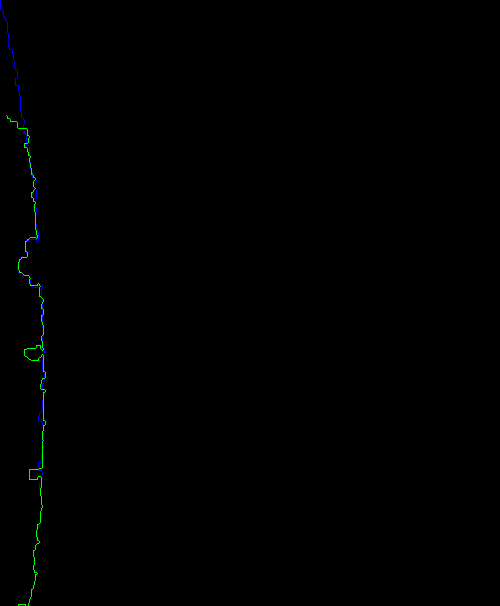
\includegraphics[width=\textwidth]{images/0.24225865209471767contours.png} % first figure itself
        \caption*{(b)}
    \end{minipage}\hfill
    \caption{(a) Konturen K1 und K2 so positioniert wie sie in den
    Ursprungsbildern gefunden wurde.
    (b) Konturen, transformiert mit größter Überlappung, 
        Grad der Überlappung: 24,26 \%}
        \label{fig:k1_and_k2}
\end{figure}

\section{Visuelle Darstellung des Stitching Prozesses}

In Abbildung \ref{fig:stitching_all} ist der Prozess des Verfahrens zu sehen.
K1 ist in blau dargestellt, K2 in grün.
In jeden Bild ist der Grad der Überlappung dargestellt. Es ist dargestellt, wie
Kontur K2 über K1 geschoben wird, um den besten Grad der Übereinstimmung zu ermitteln.
Die Bilder sind repräsentativ ausgewählt, im tatsächlichen Prozess wird K1 komplett 
über K2 bewegt.

\begin{figure}[h]
    \centering
    \begin{minipage}{0.24\textwidth}
        \centering
        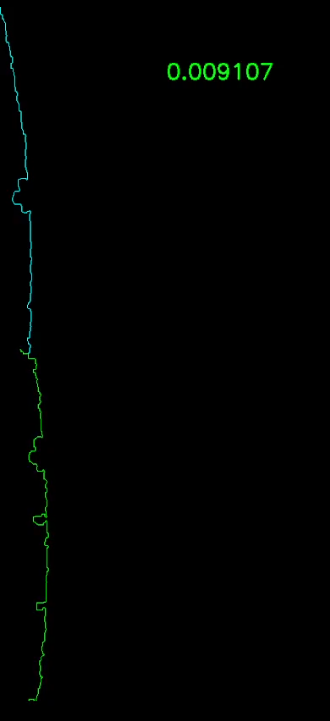
\includegraphics[width=\textwidth]{images/stitching_beginn.PNG} % first figure itself
        \caption*{(a)}
    \end{minipage}\hfill
    \begin{minipage}{0.24\textwidth}
        \centering
        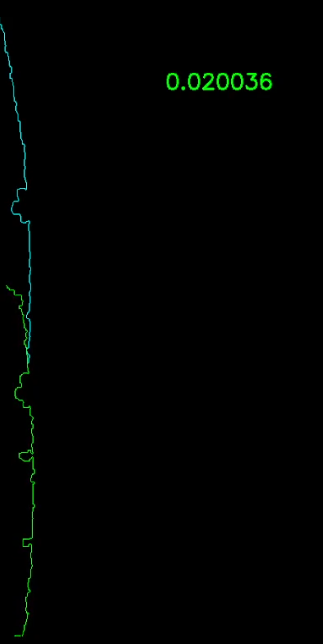
\includegraphics[width=\textwidth]{images/stitching_middle.PNG} % first figure itself
        \caption*{(b)}
    \end{minipage}\hfill
    \begin{minipage}{0.24\textwidth}
        \centering
        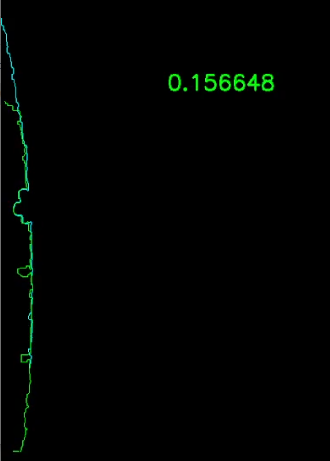
\includegraphics[width=\textwidth]{images/stitching_match.PNG} % first figure itself
        \caption*{(c)}
    \end{minipage}\hfill
    \begin{minipage}{0.24\textwidth}
        \centering
        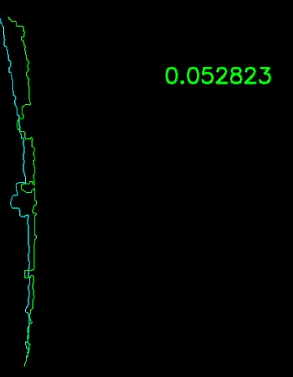
\includegraphics[width=\textwidth]{images/stitching_end.PNG} % first figure itself
        \caption*{(d)}
    \end{minipage}\hfill
    \caption{Verfahren im Verlauf dargestellt, a zu Beginn, b nach n-durchgängen, c }
    bei einem guten Match, d Kontur K2 komplett über K1 geschoben, 
    am Ende der Durchgänge.
    \label{fig:stitching_all}
\end{figure}

\section{Bilder zusammenfügen}

Nachdem alle Transformationen vorliegen wird die Transformation mit der besten 
Übereinstimmung gewählt. Diese wird genutzt, um die beiden Bilder zusammenzufügen.
Das zugehörige Bild der Konturen K2 wird transformiert, indem die Transformation 
auf jeden Pixel angewendet wird.  
Die Transformation ist nur korrekt, wenn die beiden Bilder die gleichen 
Ursprungskoordinaten haben, die auch bei den Konturen K1 und K2 verwendet wurden.

\begin{figure}[h]
    \centering
    \includegraphics[width=0.8\textwidth]{images/AM_SP0_stitched_2.png} % first figure itself
    \caption{Zusammengefügtes Bild}
    \label{fig:stitched_image}
\end{figure}

\section{Probleme und Lösungen im Verfahren}

Durch die Funktionsweise treten am Randbereich der Scandaten vermehrt Messfehler auf, 
die nicht vollständig durch vorheriges Filtern entfernt werden können. 
Damit diese Messfehler das Stitching nicht verfälschen, werden alle Konturen nochmals 
gefiltert. Alle Punkte in einer Kontur, die sich in einem konfigurierbaren 
Abstand zu den Bildrändern befinden, werden entfernt. Dadurch werden sie bei der 
Berechnung der Transformation nicht verwendet. 
Der konfigurierbare Abstand muss beim Stitching des finalen Bilds berücksichtigt 
werden und von der Transformation abgezogen werden.

Wenn Konturen mit einem großen Längenunterschied verglichen werden, 
kann eine sehr hohe Übereinstimmung ermittelt werden, die aber keine 
tatsächliche Übereinstimmung ist. Dies liegt daran, dass es wahrscheinlicher ist 
eine Sequenz mit fünf Pixeln in einer anderen Sequenz mit 500 Pixeln zu finden.  
Das kann zum Beispiel vorkommen, wenn Konturen 
die am linken und rechten Bildrand in Abbildung \ref{fig:cons} zu sehen sind, 
verglichen werden. Um dies zu vermeiden wird eine Bedienung eingeführt, dass die Länge
der Konturen nicht zu sehr voneinander abweichen darf. Bei einer Abweichung von mehr als
200 Punkten in einer Kontur sollte die Konturen nicht miteinander verglichen werden.

Auch Konturen mit einer Länge von weniger als 100 Punkten sollten nicht berücksichtigt 
werden. Diese beschreiben keine Features in einem Bild, die für das Stitching verwendet 
werden sollten. Diese Konturen beschreiben meist nur Messfehler oder 
Oberflächenstrukturen, die nicht konsistent in beiden Bildern von dem Scanner erkannt 
werden können.

Um das Ergebnis noch weiter zu verbessern, können zwei Konturen zweimal miteinander 
verglichen werden. Während des zweiten Vergleichs wird die Zielkontur mit der 
Ursprungskontur vertauscht. So wird aus beiden Konturen jeweils einmal ein fester 
Punkt gewählt. Wieder wird die Transformation gespeichert mit der besten Überlappung.
Wenn die Überlappung im zweiten Vergleich eine höhere Übereinstimmung hat, muss die 
berechnete Transformation invertiert werden. Geschieht dies nicht, kann die 
Transformation nicht für den finalen Stitchprozess eingesetzt werden, weil dort 
das Ziel und Ursprungsbild fest gesetzt ist.


\chapter{Spannkraftinduzierten Deformation}

Im folgenden Kapitel wird die Methode zur Erkennung und Analyse von durch 
Spannkraft induzierter Deformationen beschrieben. Ziel ist es, 
aus zwei zusammengefügten Bilder von zwei verschiedenen Spannungsstufen, 
Deformationen zu erkennen.
Als Deformation wird eine äußerliche Veränderung des betrachteten Bauteils bezeichnet, 
die äußere Veränderung ist hierbei über den Unterschied der Ränder der Bauteile definiert.
Bevor eine Deformation erkannt werden kann, muss die Randgeometrie von beiden
abgebildeten Bauteilen erfasst werden.
Vorerst werden in einem Schritt immer nur zwei Spannungsstufen miteinander verglichen 
und die Deformationsdaten anschließend abgespeichert.
Die Auswertung der resultierenden Daten erfolgt in einem separaten Schritt, so können auch
mehrere Spannungsstufen untereinander verglichen werden, ohne das die Komplexität steigt.

\section{Deformation zwischen zwei Spannungszuständen}

Wie beschrieben, ist die Deformation zwischen zwei Bauteilen als Differenz der 
Randgeometrie deformiert. Um die Randgeometrie eines Bauteils zu ermitteln, 
kann erneut die Kontursuche [VERWEIS] angewendet werden. Die gefundenen Konturen bilden dann 
die Ränder des Bauteils ab. So werden äußere aber auch innere Geometrien 
abgebildet und ermöglichen die Deformationserkennung. 
In Abbildung \ref{fig:stichted_contour} ist ein 
zusammengefügtes Bild und die erkannte Randgeometrie eines Bauteils zu sehen.

\begin{figure}[H]
    \centering
    \begin{minipage}{0.49\textwidth}
        \centering
        \includegraphics[width=\textwidth]{images/FDM_sp0_stitched.jpg} % first figure itself
        \caption*{(a)} 
    \end{minipage}\hfill
    \begin{minipage}{0.49\textwidth}
        \centering
        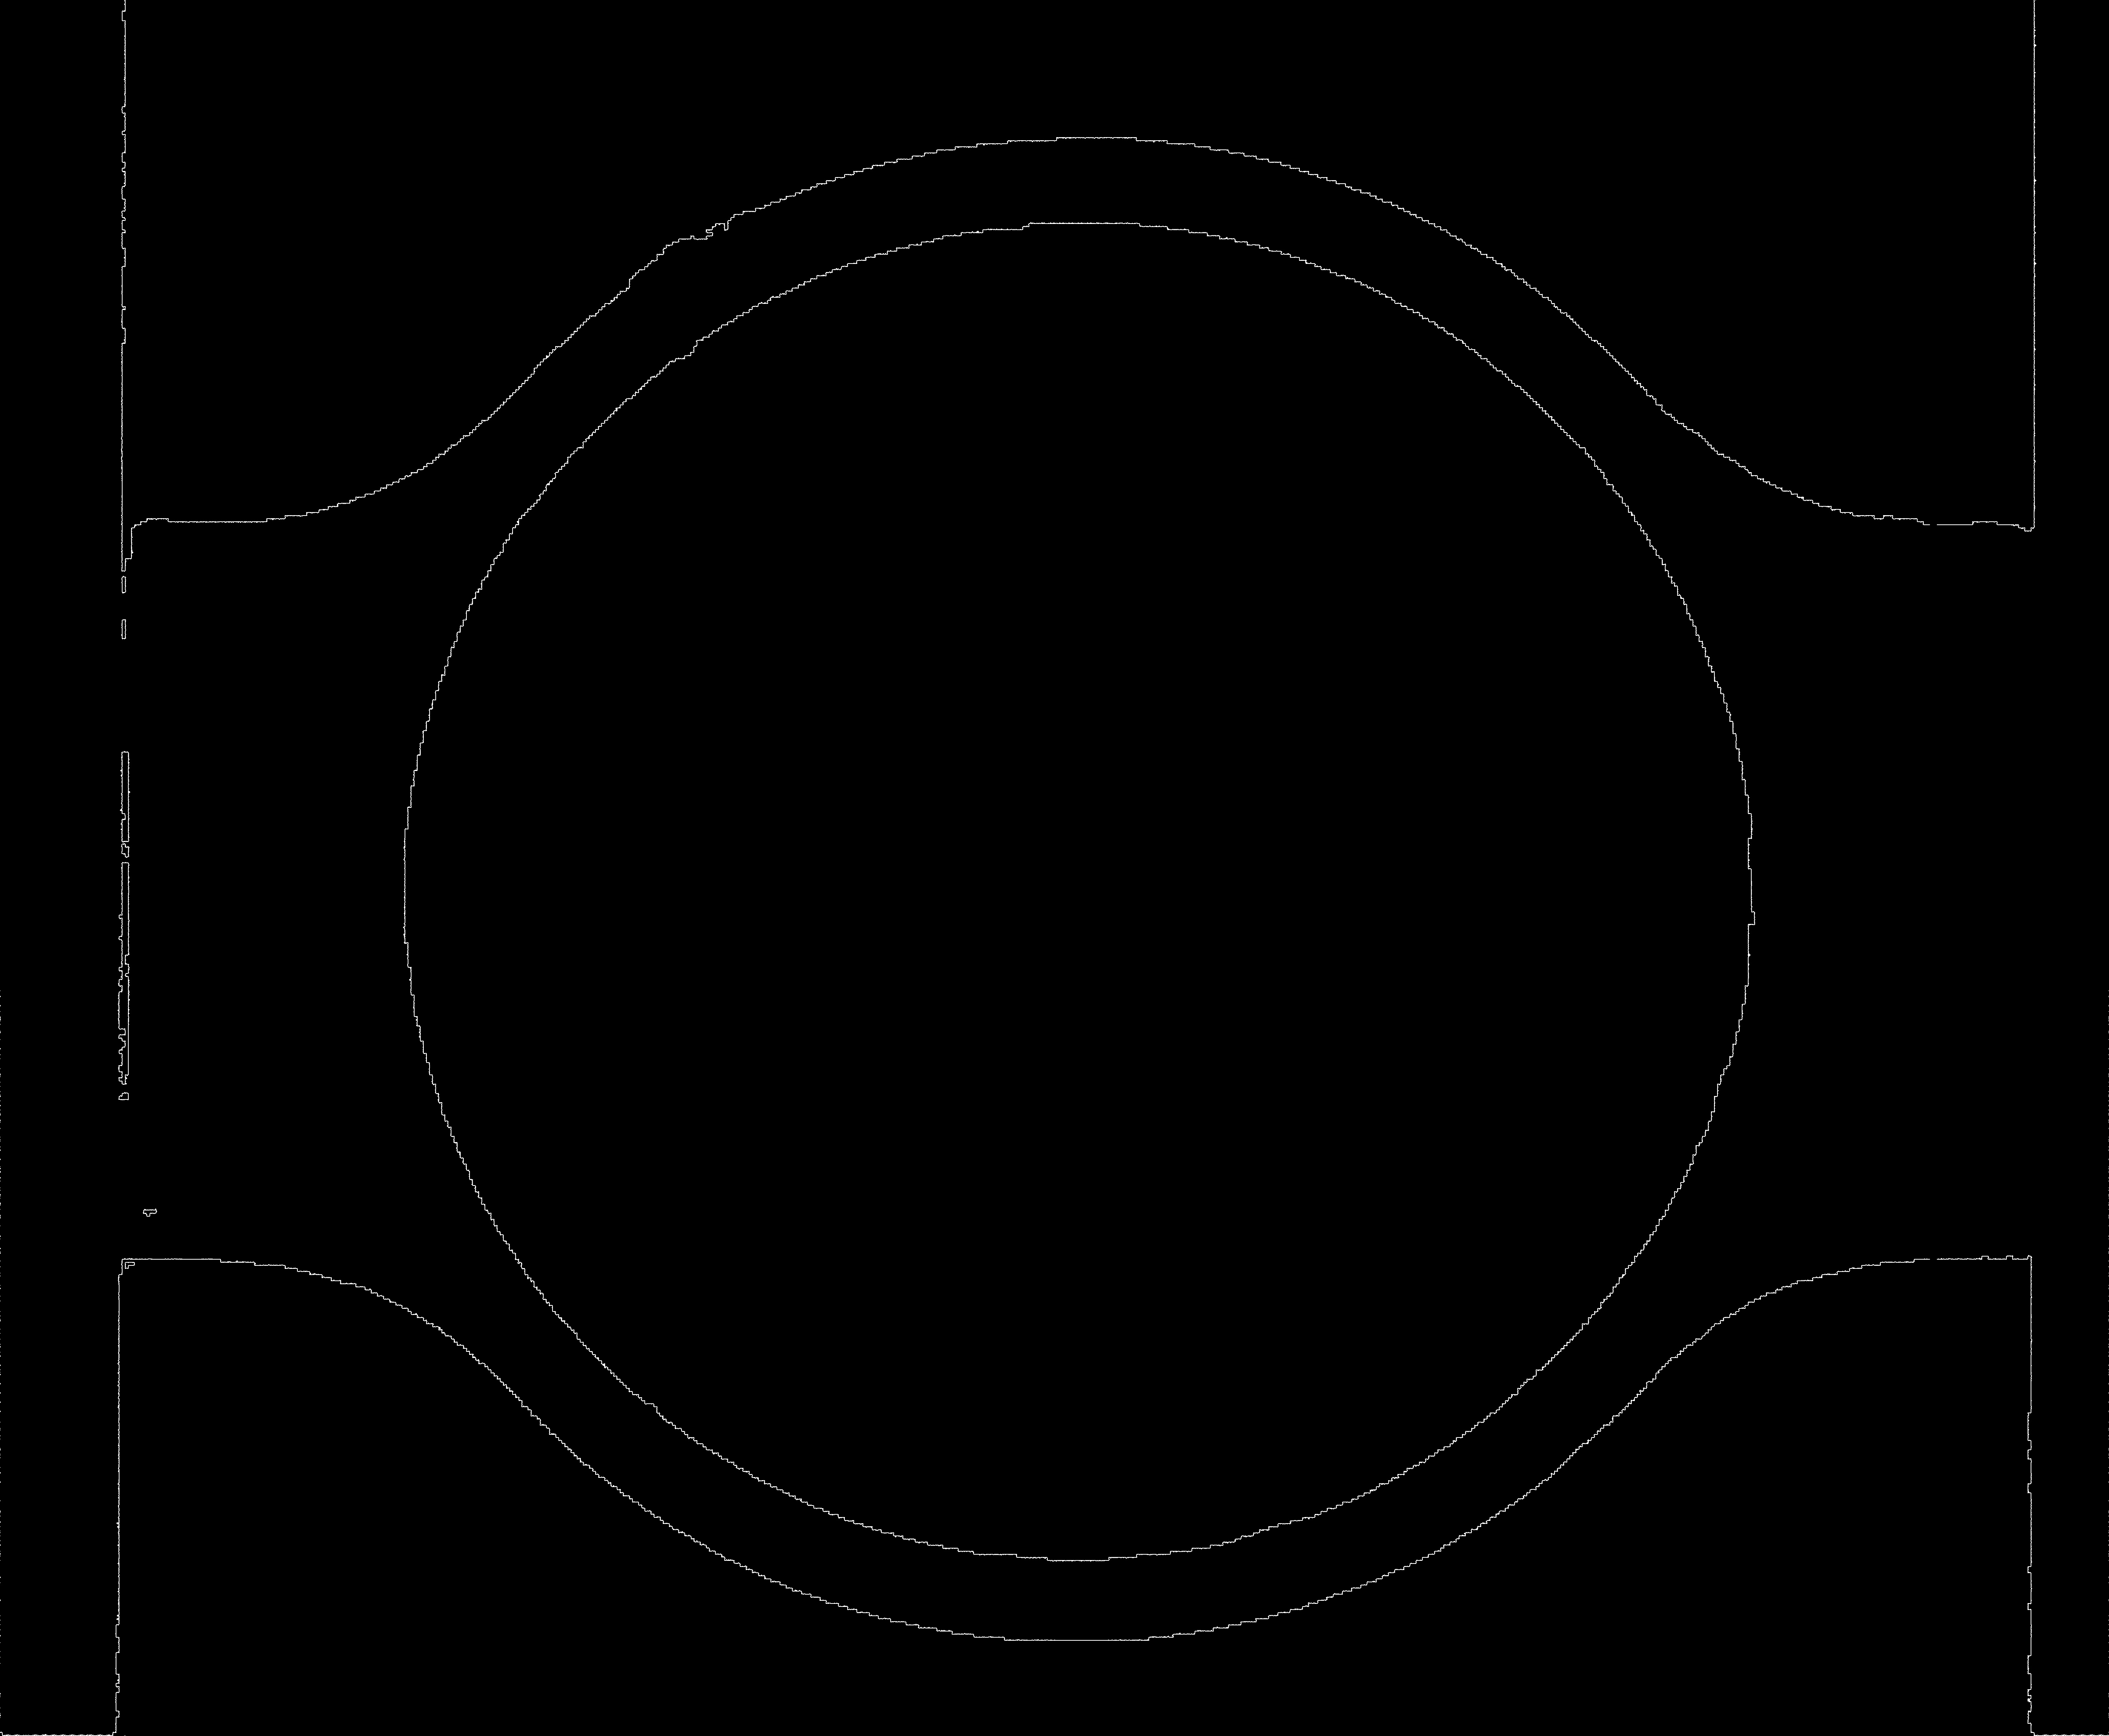
\includegraphics[width=\textwidth]{images/contours_FDM_sp0_stitched.jpg} % first figure itself
        \caption*{(b)}
    \end{minipage}\hfill
    \caption{(a) Zusammengefügtes Bild des FDM Demonstratorbauteils, Spannungsstufe 0
    (b) Randgeometrie von (a), die zur Erkennung der Deformation genutzt wird}
        \label{fig:stichted_contour}
\end{figure}

\subsection{Randgeometrien übereinander legen}

Um die Differenz zweier Randgeometrien bilden zu können, müssen diese übereinander 
gelegt werden.
Dies garantiert, dass die gebildete Differenz minimal ist.
Der schon beschriebe Ansatz des Konturmatching [VERWEIS] könnte auch hier genutzt worden. 
allerdings müssen hier die gesamten Konturen betrachtet werden und nicht wie zuvor nur 
der überlappende Auschnitt. Das schon vorgestellte Verfahren ist für die Konturen eines
gesamten Bauteils nicht performant genug um eine akzeptable Laufzeit für das Verfahren
zu gewährleisten. 
Deswegen wird hier ein anderes Verfahren eingesetzt. Es basiert auf demselben Prinzip,
Punktepaare zu finden deren euklidischen Distanz gleich null ist. Anstatt das aber 
jeder Punkt der Zielkontur mit jedem Punkt der Ursprungskontur verglichen wird, 
wird ein maximaler Radius definiert in dem nach benachbarten Punkten gesucht wird.
Hierfür muss die Kontur erst in eine zweidimensionale Datenstruktur überführt werden.
Dieser zusätzliche Aufwand sorgt für eine deutlich verkürzte Laufzeit.

Ähnlich zu dem schon beschriebenen ICP-Algorithmus [VERWEIS] wird eine Transformation berechnet,
mit der eine Kontur einer anderen Kontur angenähert werden kann.
Die Transformation wird mit folgendem Algorithmus berechnet:
(FRAGE: Hier entweder das, oder latex-pseudocodeblock, oder python screenshot?).

\begin{enumerate}
    \item Zu jedem Punkt in der Ursprungskontur wird der Nachbarpunkt
    in der Zielkontur gesucht, der den kleinsten euklidischen Abstand besitzt.
    \item Wird kein solcher Punkt in einem definierten Radius gefunden,
    wird der nächste Punkt der Ursprungskontur
    betrachtet. Falls ein Punkt gefunden wurde, wird der Vektor gebildet der die Punkte
    der Ursprungs- und Zielkontur verbindet.
    \item Wenn alle Punkte der Ursprungskontur betrachtet sind, wird der 
    Durchschnitt aller gefunden Vektoren gebildet.
    \item Da die Transformation auf Pixel angewendet wird, muss sie ganzen Zahlen 
    entsprechen. Wenn der Absolutwert beider Vektorelemente der Transformation 
    unter 0.2 Pixel fällt wird die Transformation auf (0, 0) gerundet.
    Ansonsten wird auf die nächste ganze Zahl gerundet.
\end{enumerate}

Ist die Transformation ungleich dem Vektor (0, 0) wird sie auf die Ursprungskontur 
angewendet und erneut die Transformation berechnet. Dies wird so lange wiederholt bis 
die Transformation dem Nullvektor entspricht. Wenn dies geschieht, sind beide Konturen, 
und damit die Randgeometrien der Bauteile angenähert.
Um Rechenzeit zu sparen werden vor dem Ermitteln der ersten Transformation die 
Massenmittelpunkte beider Bauteilgeometrien berechnet und übereinader gelegt.

\subsection{Deformation messen}

[Deformation ausführlich beschreiben]
Nachdem die beschriebenen Schritte erfolgt sind, kann die Deformation bestimmt werden.
Hierfür wird über die gesamte x-Achse des Bildes iteriert und die kleinste Differenz 
zwischen zwei Punkten gebildet. Diese entspricht dann einer Abweichung. 
Da innere und äußere Randgeometrie separat betrachtet werden, kann es immer nur zwei
solcher Punktepaare geben, eins am oberen Ende des Bauteils und eins am unteren Ende.
Es wird der euklidische Abstand beider Punktepaare gebildet und aufsummiert.
So entsteht ein Datensatz für ein Bild, 
dass die Differenz zweier Spannungsstufen ausgibt. In Abbildung \ref{fig:deformation_data}
ist ein solcher Datensatz zu sehen. 

Innere und äußere Randgeometrien werden separat betrachtet und analysiert.
In Abbildung \ref{fig:deformation_data_vis} ist die Deformation des inneren Kreises
visuell dargestellt. In Abbildung \ref{fig:deformation_data_graph} sind die 
Deformationswerte grafisch dargestellt.

Es wurde ein per FDM gefertigtes Bauteil eingespannt und zwei Spannungsstufen verglichen.
Die Blau sehende Linie bildet die Randgeometrie des Bauteils ab, dass mit Spannungsstufe
null eingespannt wurde. Das entspricht hier nur einer lockerer Einspannung bei 

\begin{figure}[H]
    \centering
    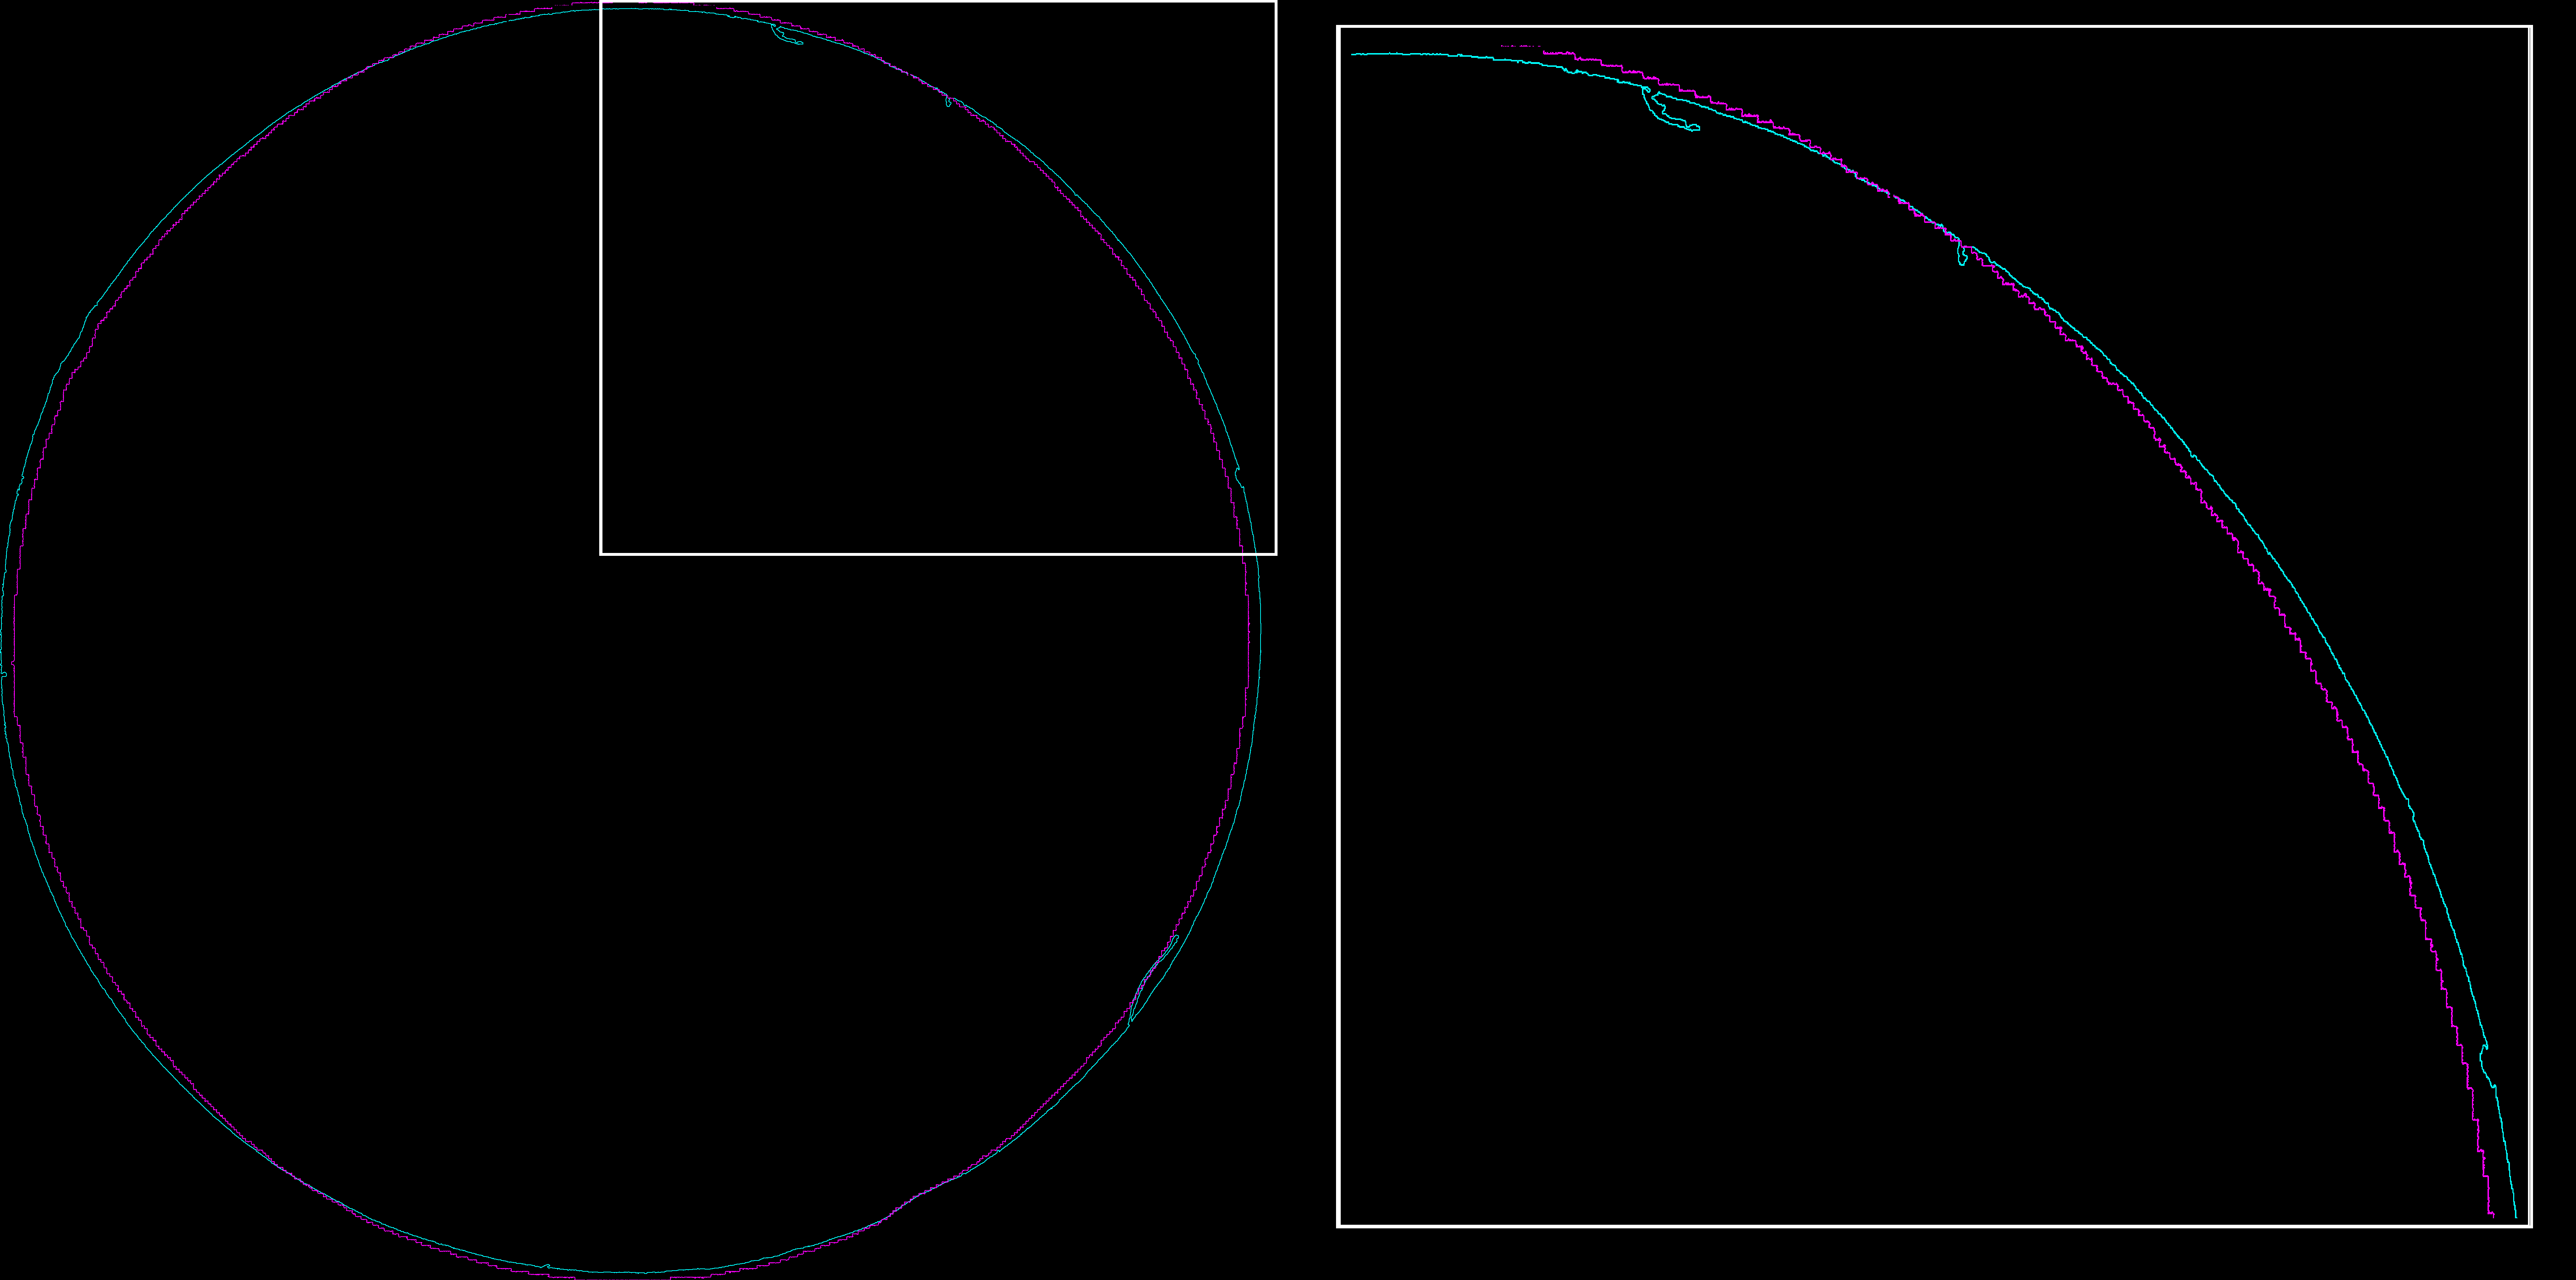
\includegraphics[width=0.99\textwidth]{images/FDM2_SP0_stitched_FDM2_SP4_stitched_1_1_cut.png}
    \caption{Deformation der inneren Bauteilgeometrie des Demonstratorbauteils 
    visuell dargestellt}
    \label{fig:deformation_data_vis}
\end{figure}


\begin{figure}[H]
    \centering
    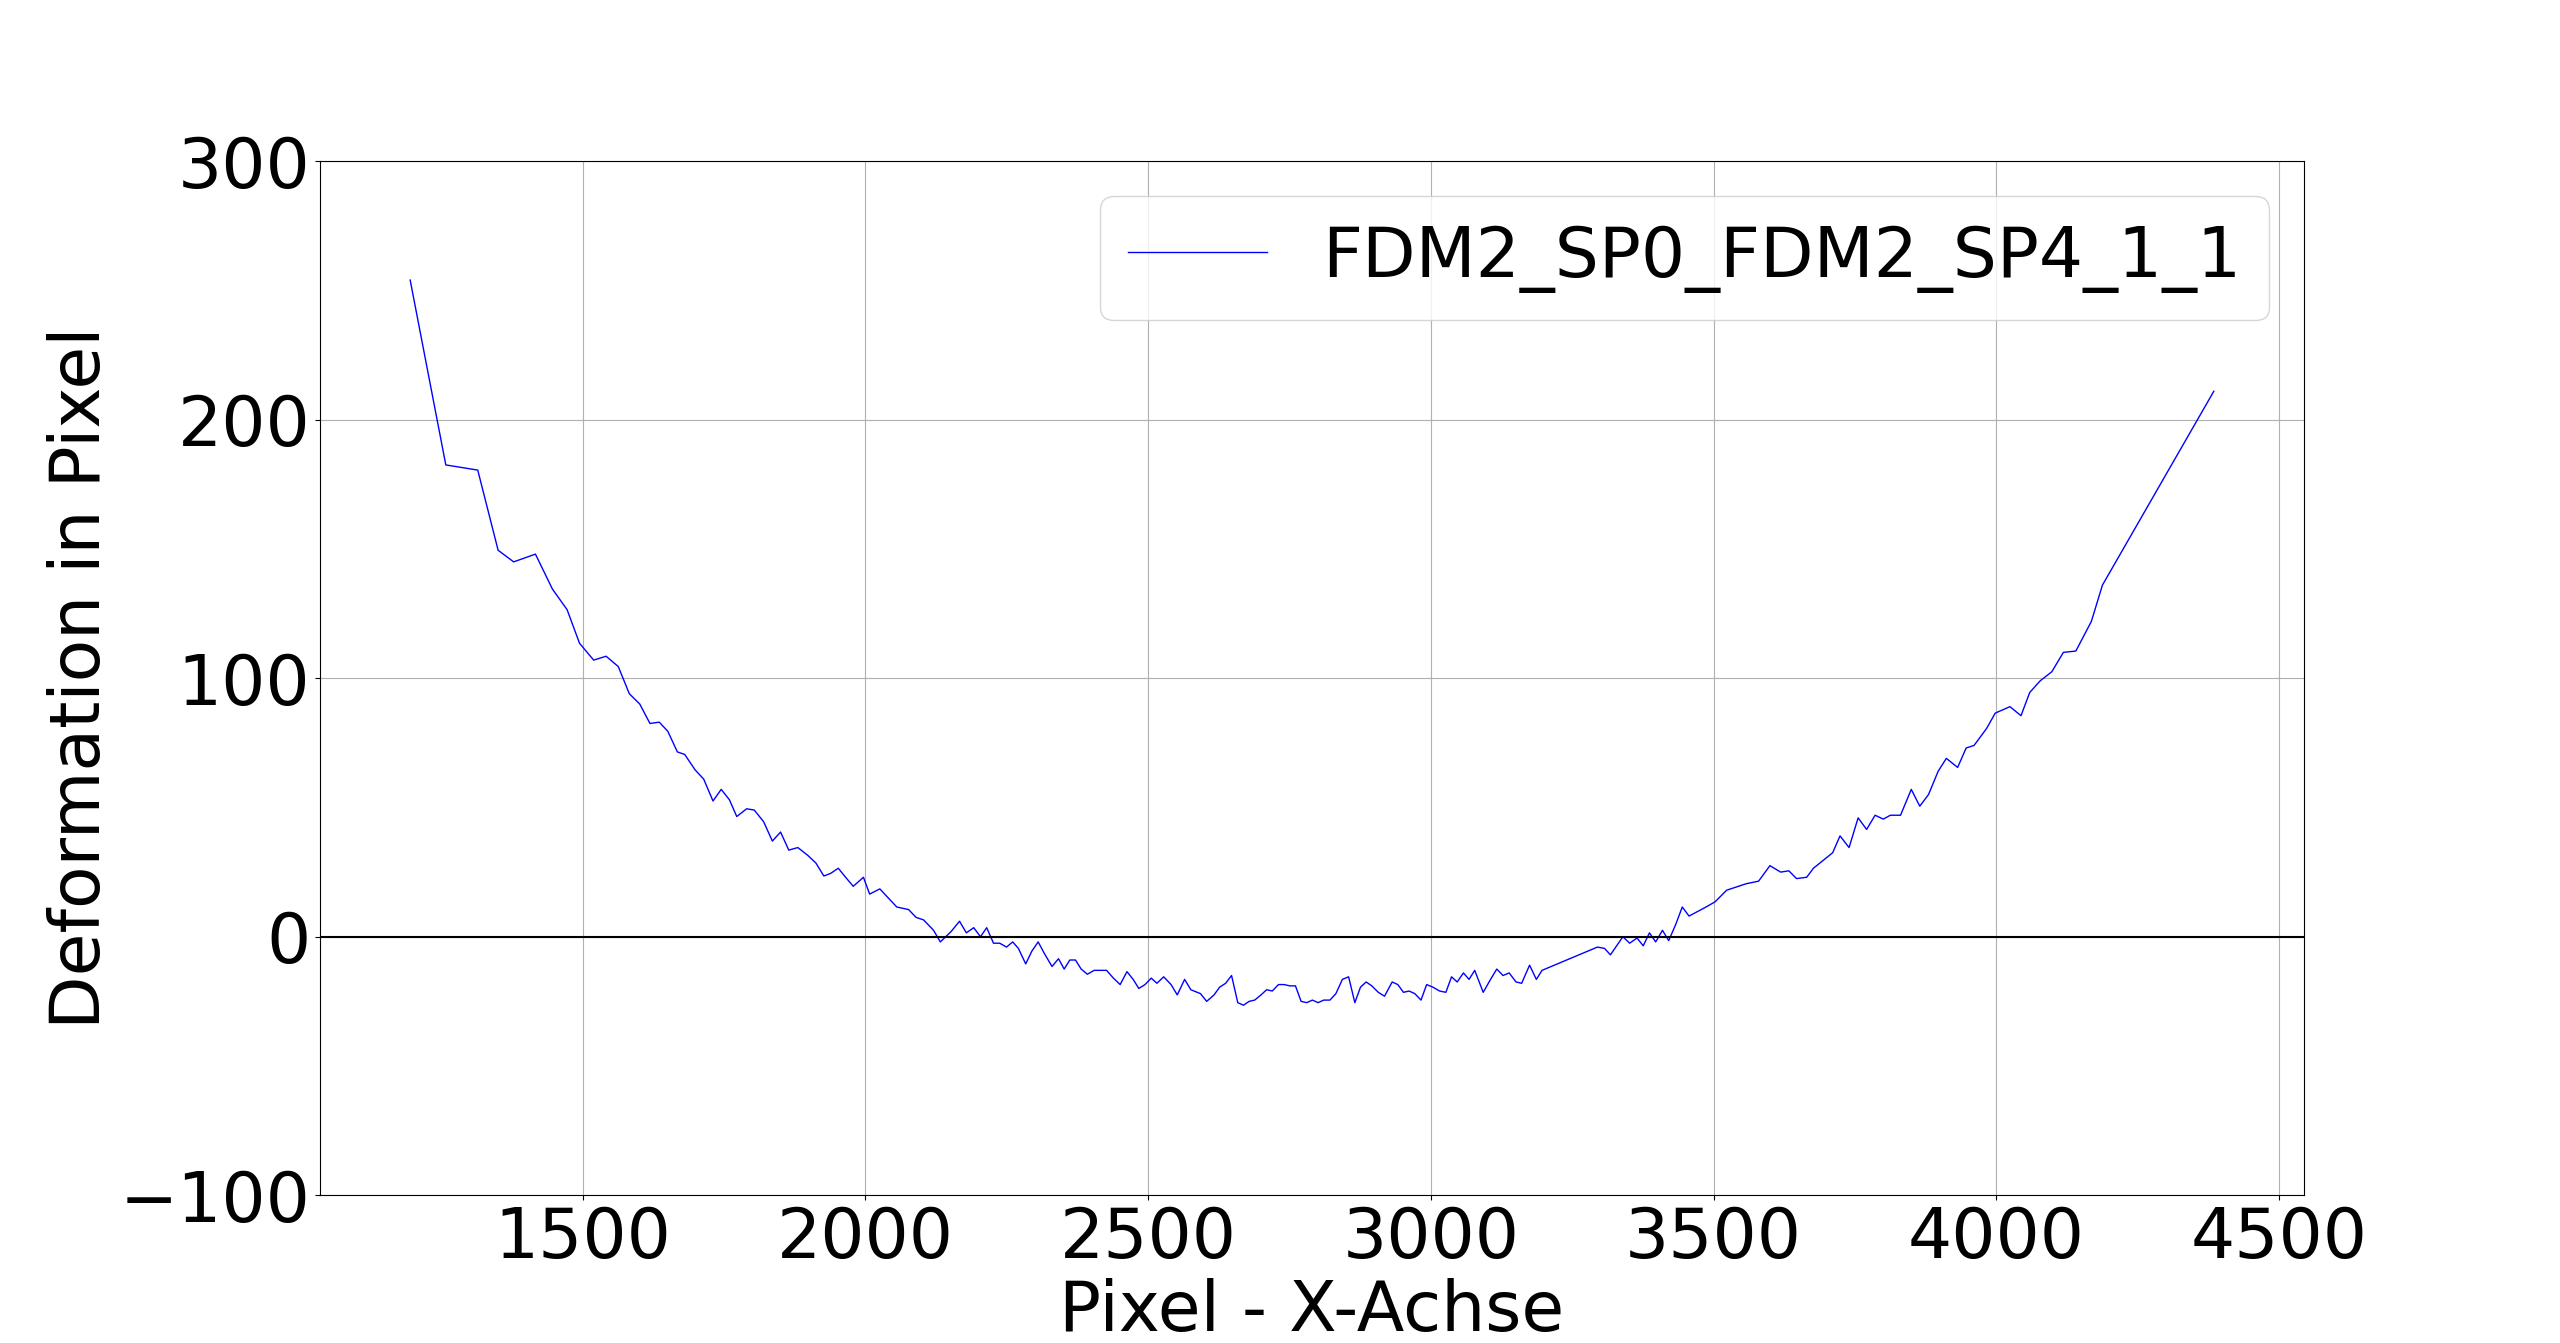
\includegraphics[width=0.9\textwidth]{images/FDM_sp0_sp4_inner.png}
    \caption{Deformation der inneren Bauteilgeometrie 
    des Demonstratorbauteils als Graph}
    \label{fig:deformation_data_graph}
\end{figure}

Es ist gut zu erkennen, dass sich das Bauteil 
im mittleren Bereich ausgedehnt hat und in den Randbereichen schmaler geworden ist.
Dieser Datensatz unterliegt einer relativ großen Streuung. Um mehrere Spannungsstufen
zu vergleichen, wird der Datensatz zu einer Geraden zusammengefasst.
Diese Gerade ist auch in \ref{fig:deformation_data} in Blau zu sehen. Sie wird 
gebildet, indem immer zehn Datenpunkte zu einem zusammengefasst werden. 
So können auch mehrere Spannungsstufen visuell dargestellt und verglichen werden.

\begin{figure}[H]
    \centering
    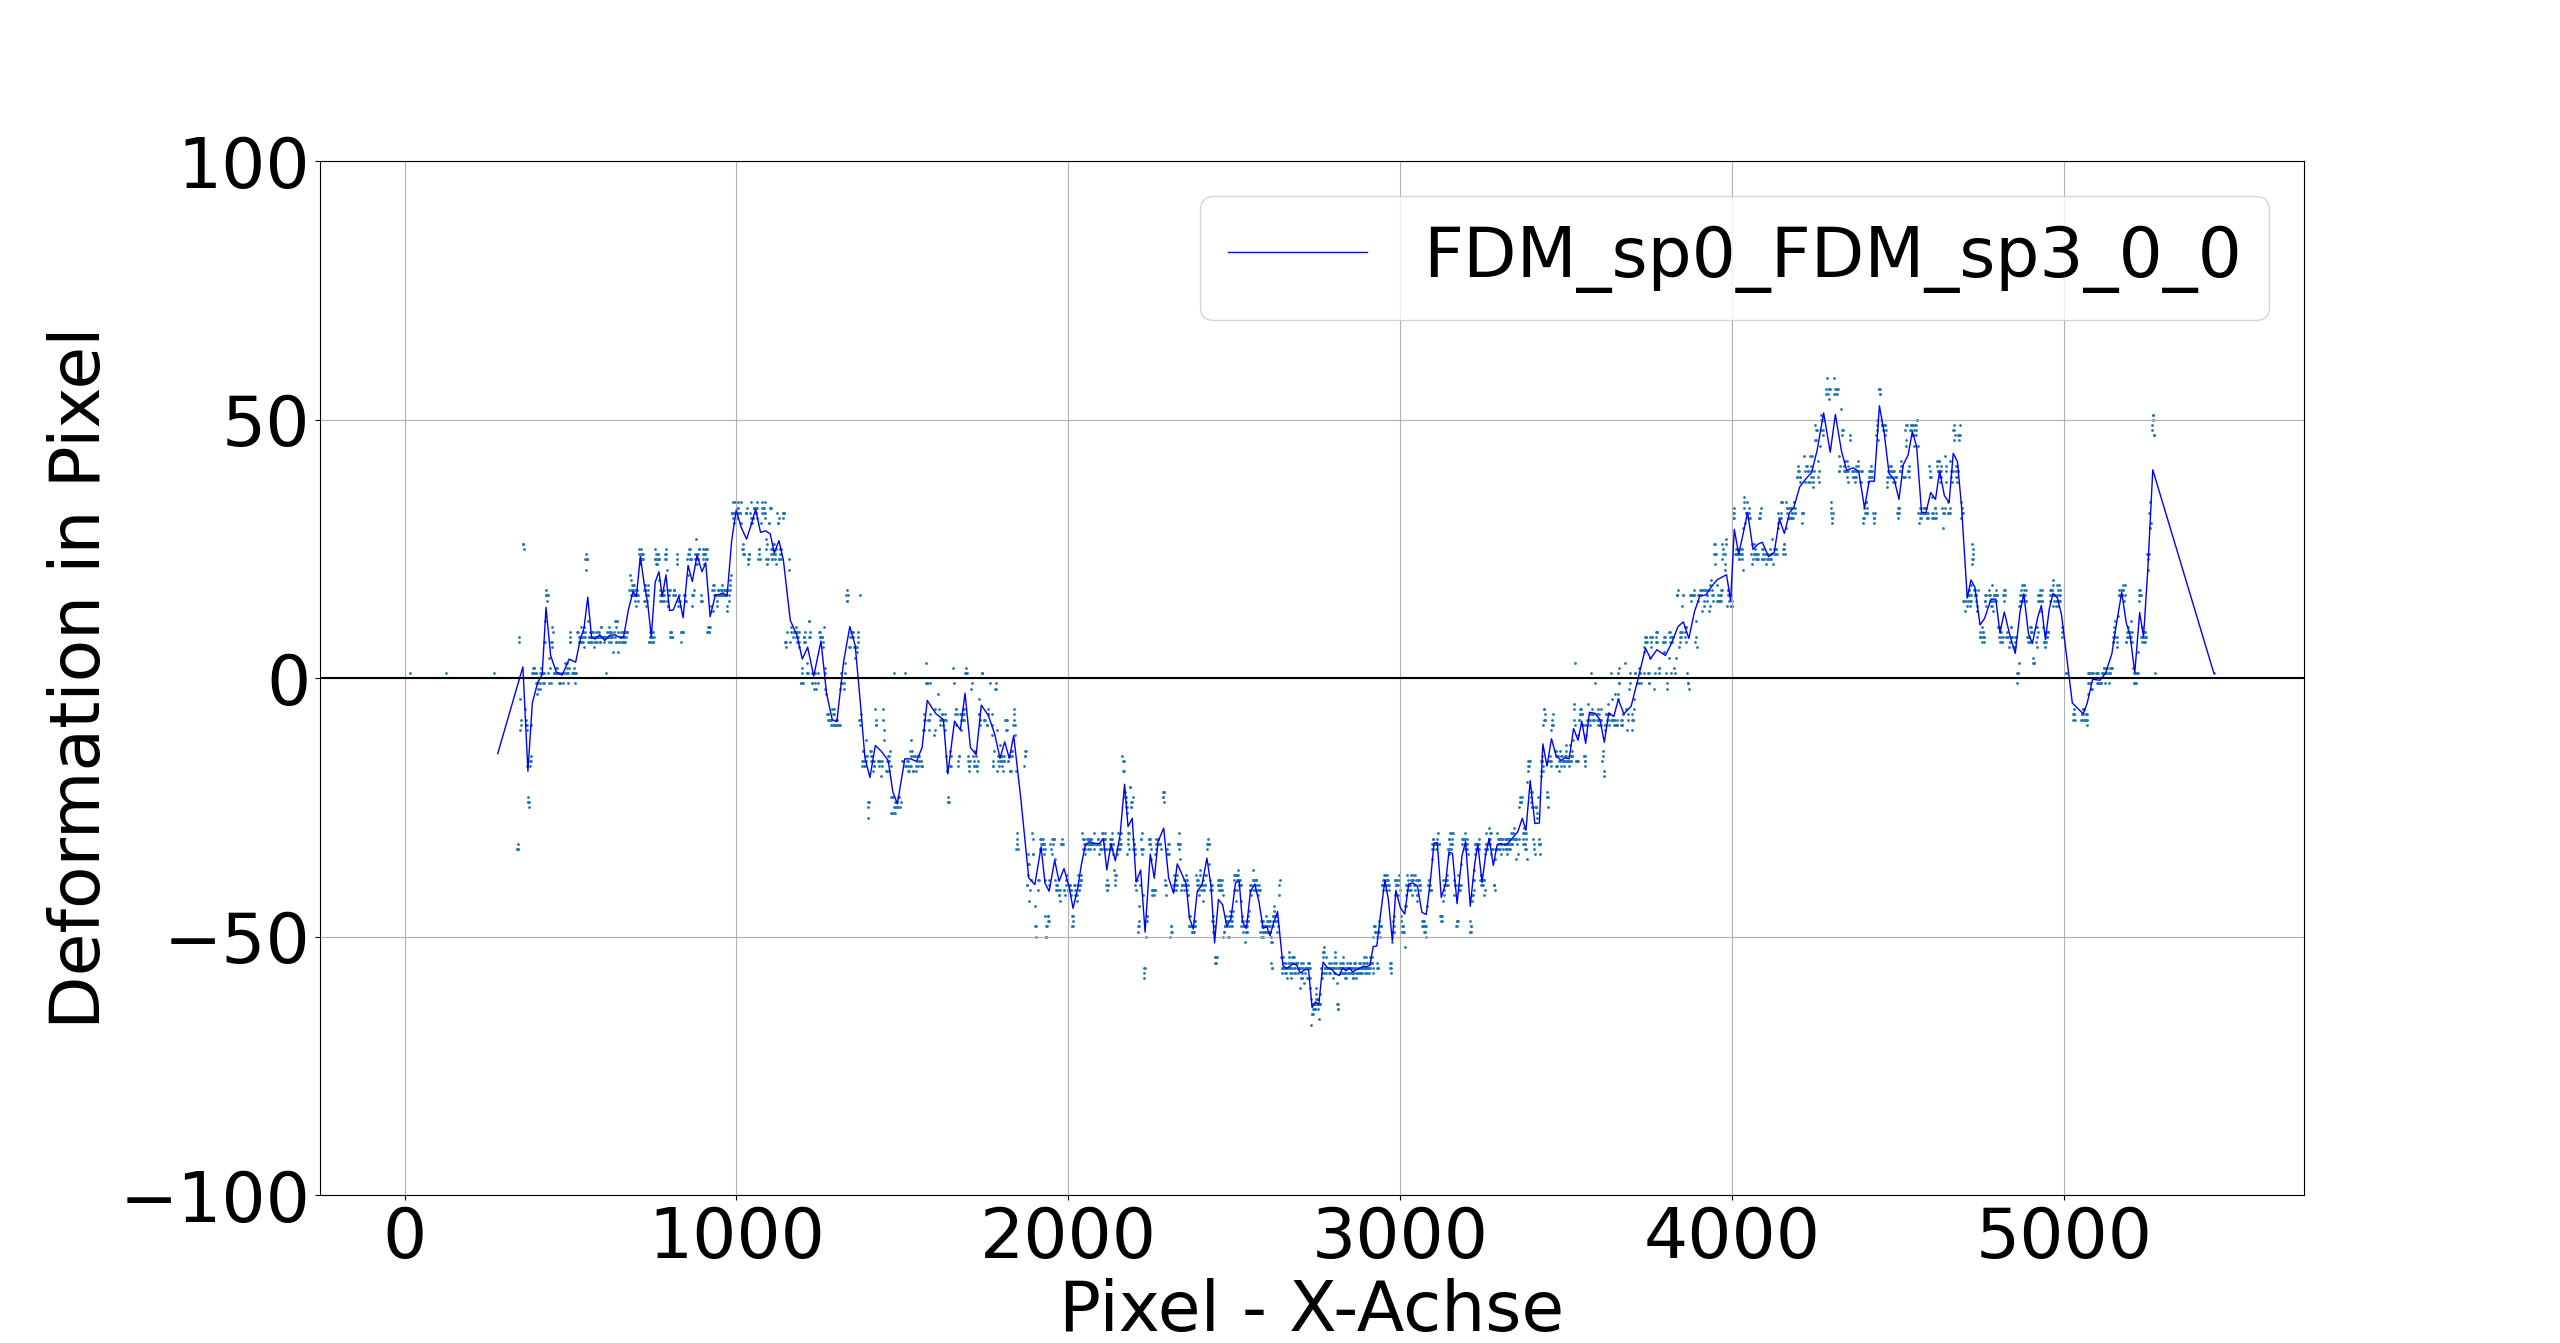
\includegraphics[width=0.7\textwidth]{images/FDM_sp0_sp3_defo_plot.png}
    \caption{Differenz von zwei Spannungsstufen bei einem FDM Bauteil, äußere 
    Bauteilgeometrie.}
    \label{fig:deformation_data}
\end{figure}

\begin{figure}[H]
    \centering
    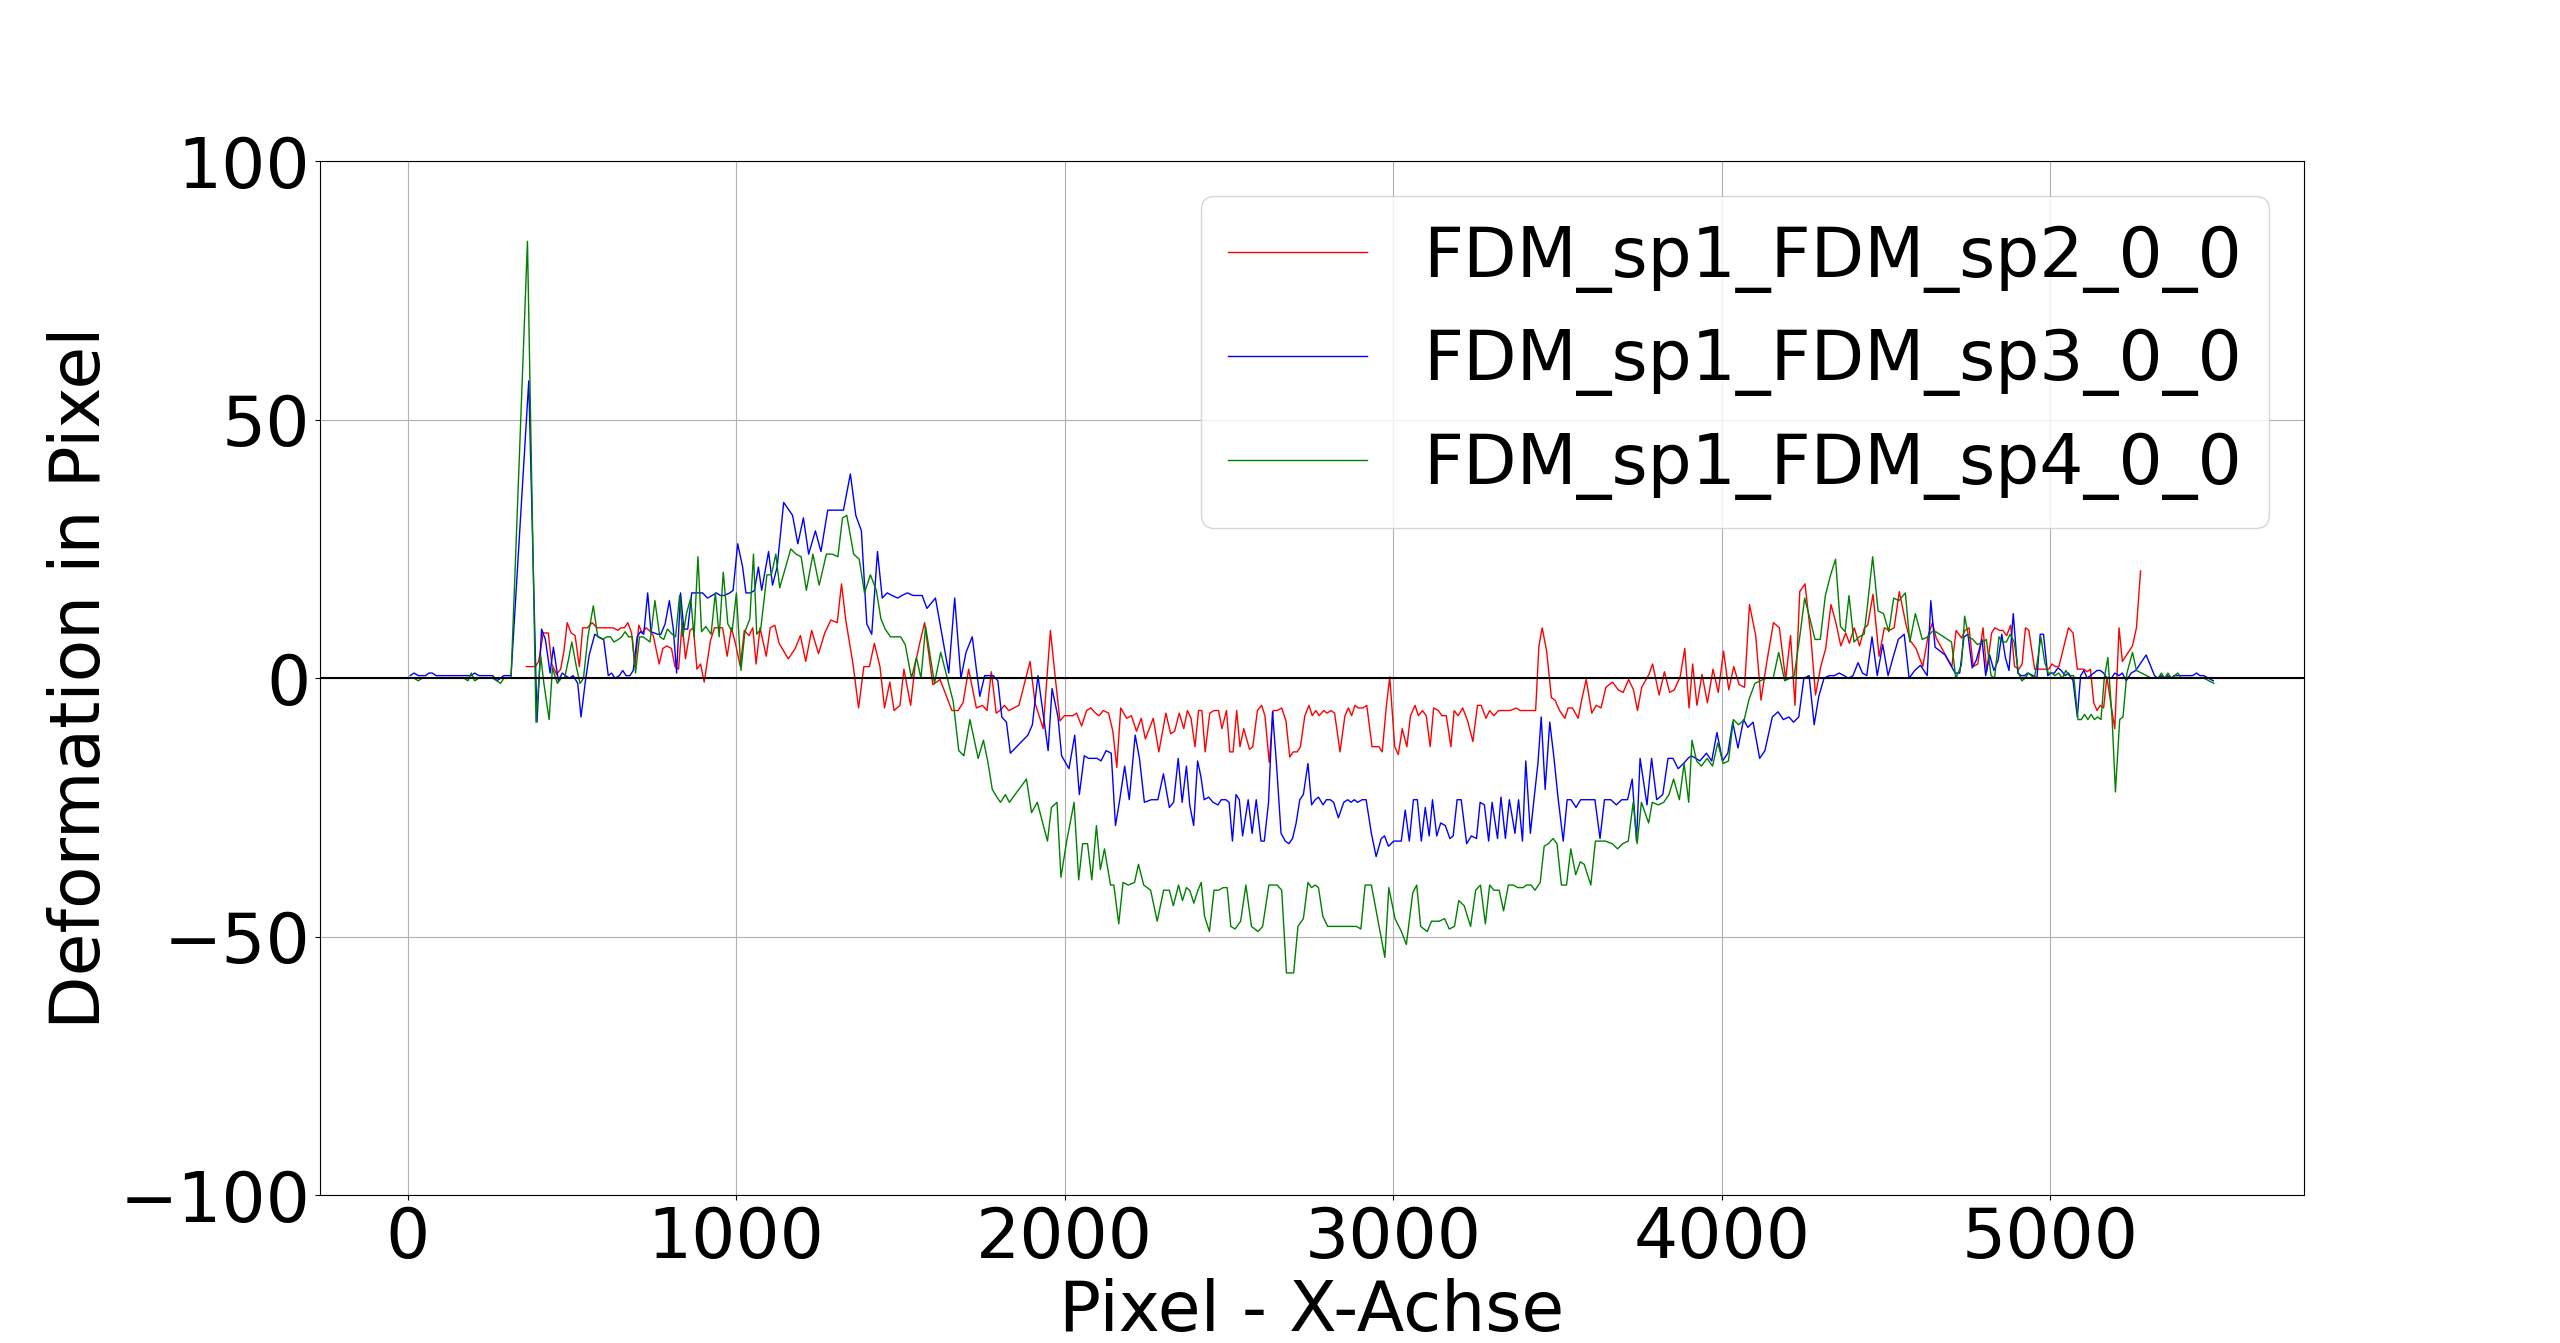
\includegraphics[width=0.7\textwidth]{images/FDM_sp0_many_defo_plot2.png}
    \caption{Differenz von mehreren Spannungsstufen bei einem FDM Bauteil}
    \label{fig:deformation_data_all}
\end{figure}





\chapter{Anwendung und Algorithmus}

Ziel dieser Arbeit ist es nicht nur eine Methodik zur optische 
Deformationserkennung zu entwickeln, sondern diese Methodik auch in einer 
Anwendung einfach nutzbar zu machen. 

Diese Kapitel dokumentiert diese Anwendung und geht auf Herausforderungen 
in der Entwicklung ein.

\section{Anwendung}

Die Anwendung beeinhaltet verschiedene Funktionen, alle Funktionen 
können separat benutzt werden. Dadurch müssen zeitintensive Vorgänge nicht 
wiederholt werden, sondern Zwischenergebnisse können abgespeichert und 
neu geladen werden.
Die Anwendung bietet Funktionen um Resultate in dem entsprechenden Dateiformat zu 
speichern. Soweit möglich werden Dateinamen Empfehlungen automatisch ermittelt, 
daher ist es zu empfehlen von Anfang an mit einem einheitlichen Namensschema bei
den 3D-Scannerdaten zu arbeiten. 
Das Schema \glqq Bauteilbeschreibung \textunderscore Spannungsstufe\grqq~~
\textunderscore Scannerdurchlauf.ply
wird empfohlen. Ein Beispiel für die zweite Pointcloud eines FDM-Bauteil bei der
vierten Spannungsstufen wäre also \glqq FDM0\textunderscore SP4\textunderscore 2.ply\grqq~.
In Abbildung \ref{fig:software_screenshot} ist die Oberfläche der Anwendung zu sehen.

\begin{figure}[H]
    \centering
    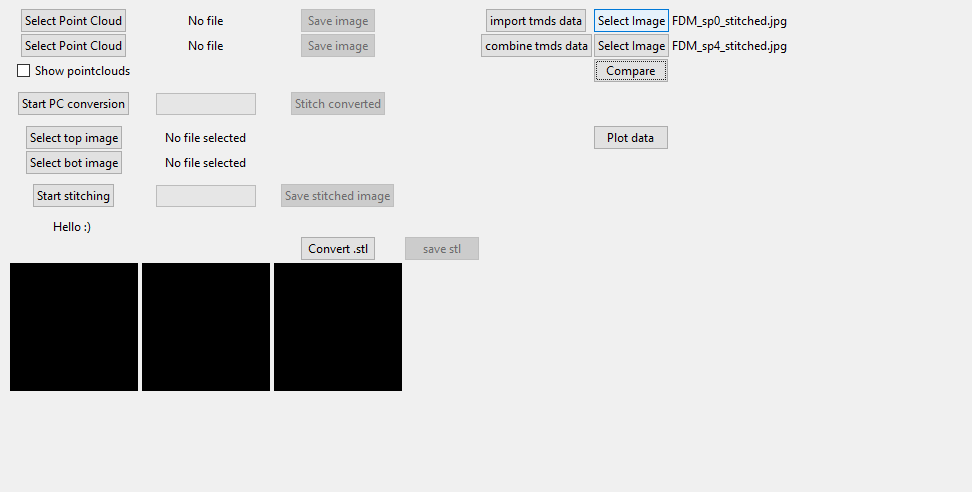
\includegraphics[width=0.9\textwidth]{images/software_screenshot.png}
    \caption{Anwendungsoberfläche}
    \label{fig:software_screenshot}
\end{figure}

Über die Buttons \glqq Select Pointcloud\grqq~ können Pointclouds zum Konvertieren in Bilder
ausgewählt werden. Der Text neben dem Bild zeigt den Dateinamen der ausgewählten 
Datei an. Die obere Pointcloud sollte hier als erstes ausgewählt werden.
Der Button \glqq Start PC conversion\grqq~~startet die Konvertierung. Der Balken 
daneben zeigt den Prozessfortschritt. 
Wenn \glqq Show Pointclouds\grqq~ gesetzt ist, werden die Pointclouds vor dem 
Konvertieren in einem separaten Fenster angezeigt. So kann überprüft werden, ob die 
korrekte Pointcloud ausgewählt wurde.
Wenn der Prozess abgeschlossen ist, werden die resultieren Bilder als Vorschau in der 
Anwendung angezeigt und die Option zum Speichern der Bilder ist nicht mehr ausgegraut.
Zusätzlich wird nach dem Konvertierungsprozess die Schaltfläche 
\glqq Stitch converted\grqq~ freigeschaltet. Durch diese Option können die 
Bilder direkt zusammengefügt werden, ohne das die Bilder extra gespeichert und 
eingeladen werden müssen. Wenn schon existierende Bilder zusammengefügt werden sollen, 
können die Schaltflächen \glqq Select top image\grqq und \glqq Select bot image\grqq
ausgewählt werden um das obere und untere Bild auszuwählen. Auch hier wird die 
ausgewählte Datei als Text angezeigt. Die Dateiauswahl erfolgt über das 
Windows-Kontextmenü, der zuletzt verwendete Ordner wird hierbei erhalten, sodass das 
zweite Bild schneller ausgewählt werden kann. 
Über den Button \glqq Start stitching\grqq wird der stitching Prozess gestartet. 
Auch hier wird der Fortschritt und das Endresultat, sobald es vorliegt, angezeigt.

Damit auch die CAD-Datei des additiv gefertigten Bauteils verglichen werden kann, 
existiert der \glqq Convert stl\grqq~ Button. Hier wird eine .stl Datei zu einem Bild 
konvertiert und kann über \glqq save stl\grqq~ gespeichert werden.

Mithilfe der rechts zu sehenden Schaltflächen können Bilder auf ihre Deformation hin 
verglichen werden. Die resultieren Deformationsdaten werden automatisch als Textdatei
in dem Ordner \glqq deformation\underline data\grqq~ gespeichert. Dieser Ordner wird automatisch 
in dem Verzeichnis erzeugt, in dem die Anwendung ausgeführt wird. 
Die erstellten Textdateien können mithilfe des Buttons \glqq Plot data\grqq~ ausgewählt 
werden, und werden automatisch als Graph angezeigt. 

Beim konvertieren und stitchen werden alle Prozesse, die nicht voneinander abhängig sind,  
nebenläufig ausgeführt. Das reduziert die Laufzeit der Prozesse.

Die Anwendung ist in Python geschrieben, rechenintensive Prozesse wurden aber mithilfe 
der Bibliothek \glqq Numba\grqq~in optimierten Maschinencode compiliert~\cite{numba}.
Dadurch ist der Konvertierungs- und Stitching-Prozess deutlich schneller geworden. 
Abbildung \ref{label} zeigt die Laufzeiten der Anwendung mit und ohne Übersetzung in 
Maschinencode.

[TODO: Bild laufzeiten einfügen]





\chapter{Validierung}

Im folgenden Kapitel wird die Deformationerkennung analysiert und überprüft.
Zur Überprüfung werden Materialeigenschaften und aufgenommene Messwerte 
mit der erkannten Deformation verglichen.

\section{Messergebnisse}

Es wurden fünf Bauteile mit verschiedenen Spannungsstufen gemessen. Für jede 
Spannungsstufe wurde die Kraft, die auf das Bauteil wirkte sowie die Verschiebung 
des Schraubstocks gemessen.
Jede Spannungsstufe wurde durch Stufenweises anziehen des Schraubstocks erreicht.
Die Spannkraftkurve eines einzelnen Einspannvorgangs ist in 
Abbildung \ref{fig:single} zu sehen. 
In der Spannungskurve ist ein elastischer Bereich für das 
Bauteil zu sehen, in dem sich die Spannkraft zurückbewegt, nachdem kein 
Anzugdrehmoment mehr anliegt. Aus diesem Grund kann nicht der maximale Wert der Spannkraft angenommen werden, 
sondern es muss ein Wert gewählt werden der nach dem maximalen Ausschlag liegt.
Dieser wurde über die erste Ableitung der Spannkraftkurve gefunden. Sobald der 
Absolutwert der Steigung unter 0.0009 N fällt, wir die Spannkraft und Auslenkung an 
diesem Punkt gewählt. 0.0009 N wurde empirisch ermittelt, um bei allen Bauteilen einen 
angemessenen Wert zu liefern.
Die Spannkraft wurde an zwei Achsen aufgenommen und zu der Gesamtkraft aufsummiert.

\begin{figure}[H]
    \centering
    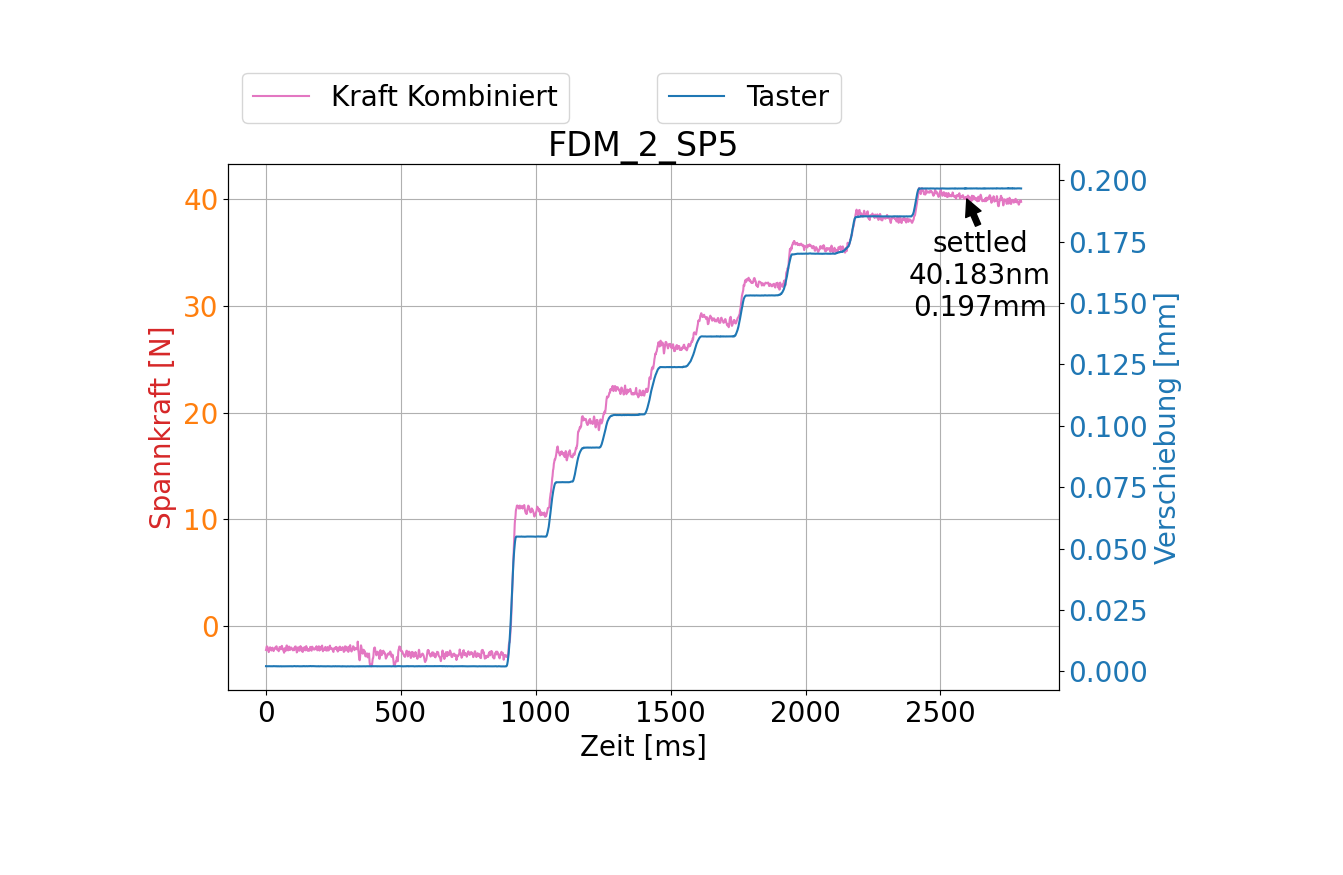
\includegraphics[width=0.99\textwidth]{images/spannkraftstufen_single.png}
    \caption{Kraft- und Verschiebung der Spannungsstufe fünf bei einem FDM Bauteil}
    \label{fig:single}
\end{figure}

Diese maximalen Werte für die Spannkraft und Auslenkung wurden für jedes Bauteil 
akkumuliert und sind in Abbildung \ref{fig:akkumulated} dargestellt. 
Die mit dem FDM-Prozess hergestellten Bauteile wurden jeweils in sechs Spannungsstufen
gemessen. Zwischen den Stufen wurde versucht, eine konstante Kraft auf das Bauteil 
auszuüben. Durch den manuellen Prozess des Anziehens des Schraubstocks war dies 
jedoch nicht immer möglich.
Die Metallbauteile unterscheiden sich durch ihren Aufbau. 
Alle basieren auf dem gleichen 3D-Modell, besitzen jedoch unterschiedliche 
Stützstrukturen. Im Bauteil AM0 ist die vollständige Stützstruktur vorhanden,
während in den Bauteilen AM1 und AM2 die Stützstruktur in unterschiedlicher 
Tiefe ausgebohrt wurde. Die Bauteile sind in Abbildung \ref{fig:am_parts} dargestellt.

Das Bauteil AM0 wurde nur mit zwei Spannungsstufen gemessen, 
da bereits bei der zweiten Stufe über 2500 N Kraft erforderlich war, 
um das Bauteil nur minimal in x-Richtung zu deformieren. Dies zeigt, 
dass die Stützstruktur einen erheblichen Einfluss auf die Verformbarkeit 
eines Bauteils hat. Beim Bauteil AM1 wurden 2500 N erst nach vier Spannungsstufen 
erreicht. Vergleicht man die Verformung in x-Richtung mit der Verformung von AM2,
 zeigt sich, dass das Bauteil ohne Stützstruktur bei ähnlicher Krafteinwirkung 
 etwa doppelt so weit in x-Richtung deformiert wurde.

 Die FDM-Bauteile wurden mit deutlich weniger Kraft eingespannt. 
 Hier wurde bei etwa 250 N gestoppt, dennoch ist die Verschiebung der 
 Teile deutlich größer als bei den AM-Bauteilen. Diese Werte wurden aufgenommen, 
 um die visuelle Deformationserkennung zu validieren.

\begin{figure}[H]
    \centering
    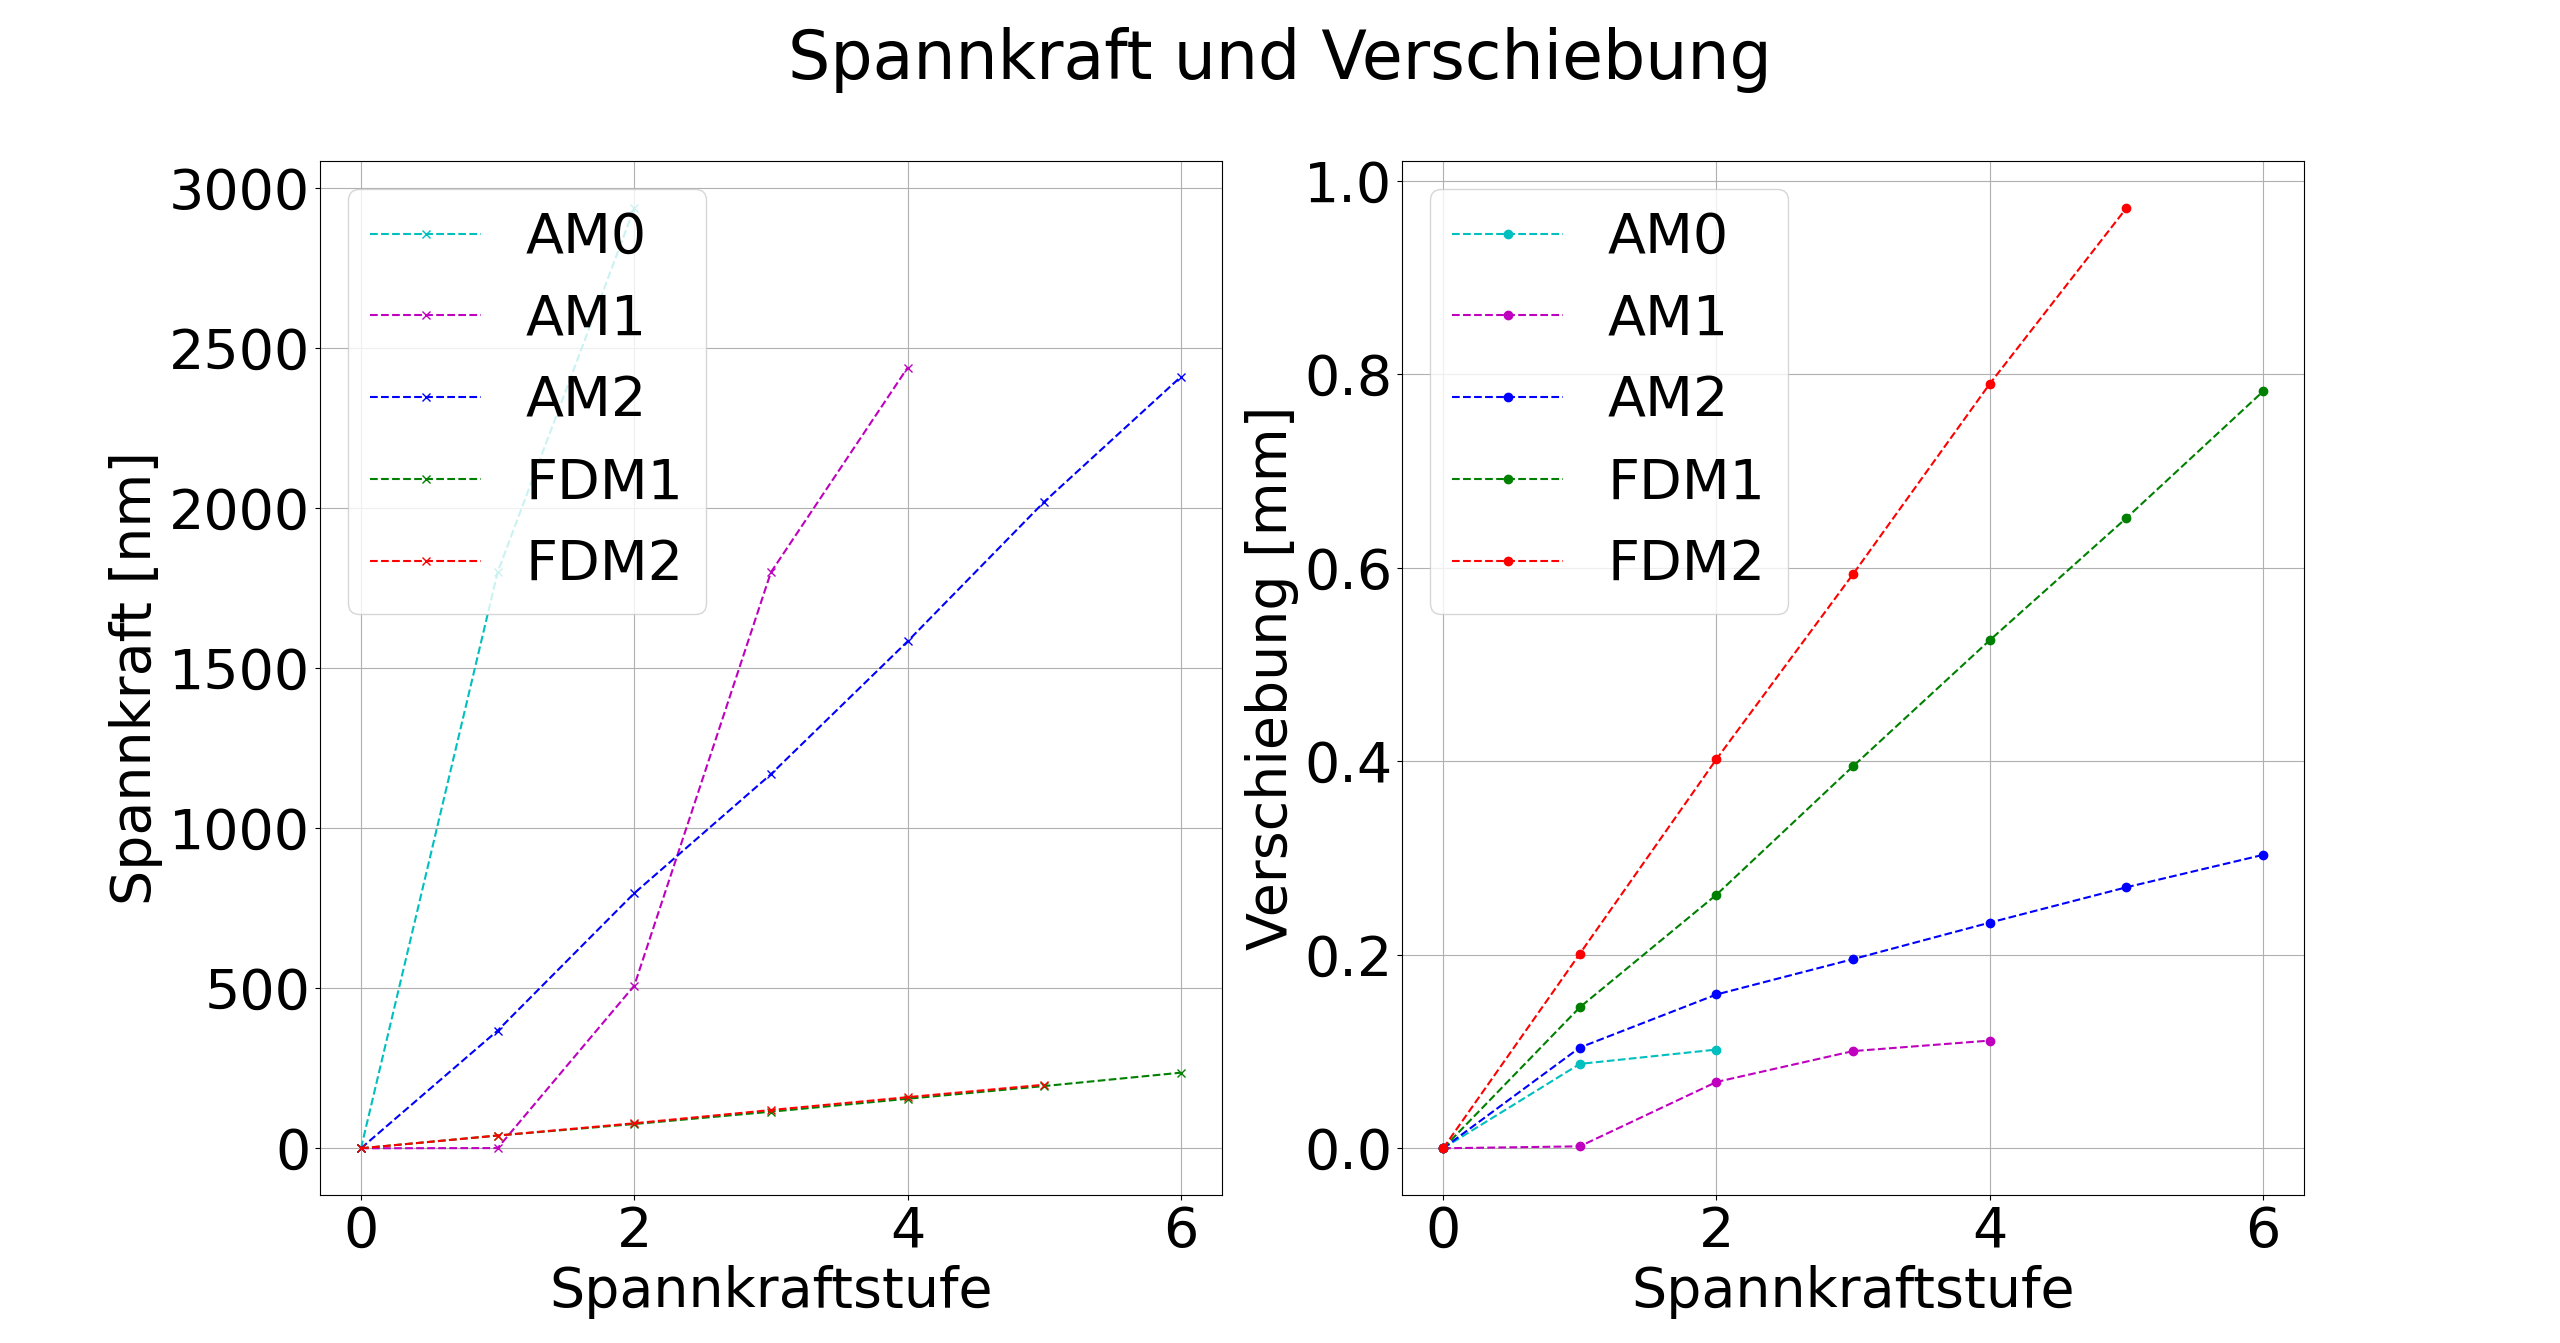
\includegraphics[width=0.99\textwidth]{images/spannkraftstufen_akkumuliert.png}
    \caption{Akkumulierte Kraft und Verschiebung, mit der jedes Bauteil deformiert wurde.}
    \label{fig:akkumulated}
\end{figure}

\begin{figure}[H]
    \centering
    \begin{minipage}{.33\textwidth}
      \centering
      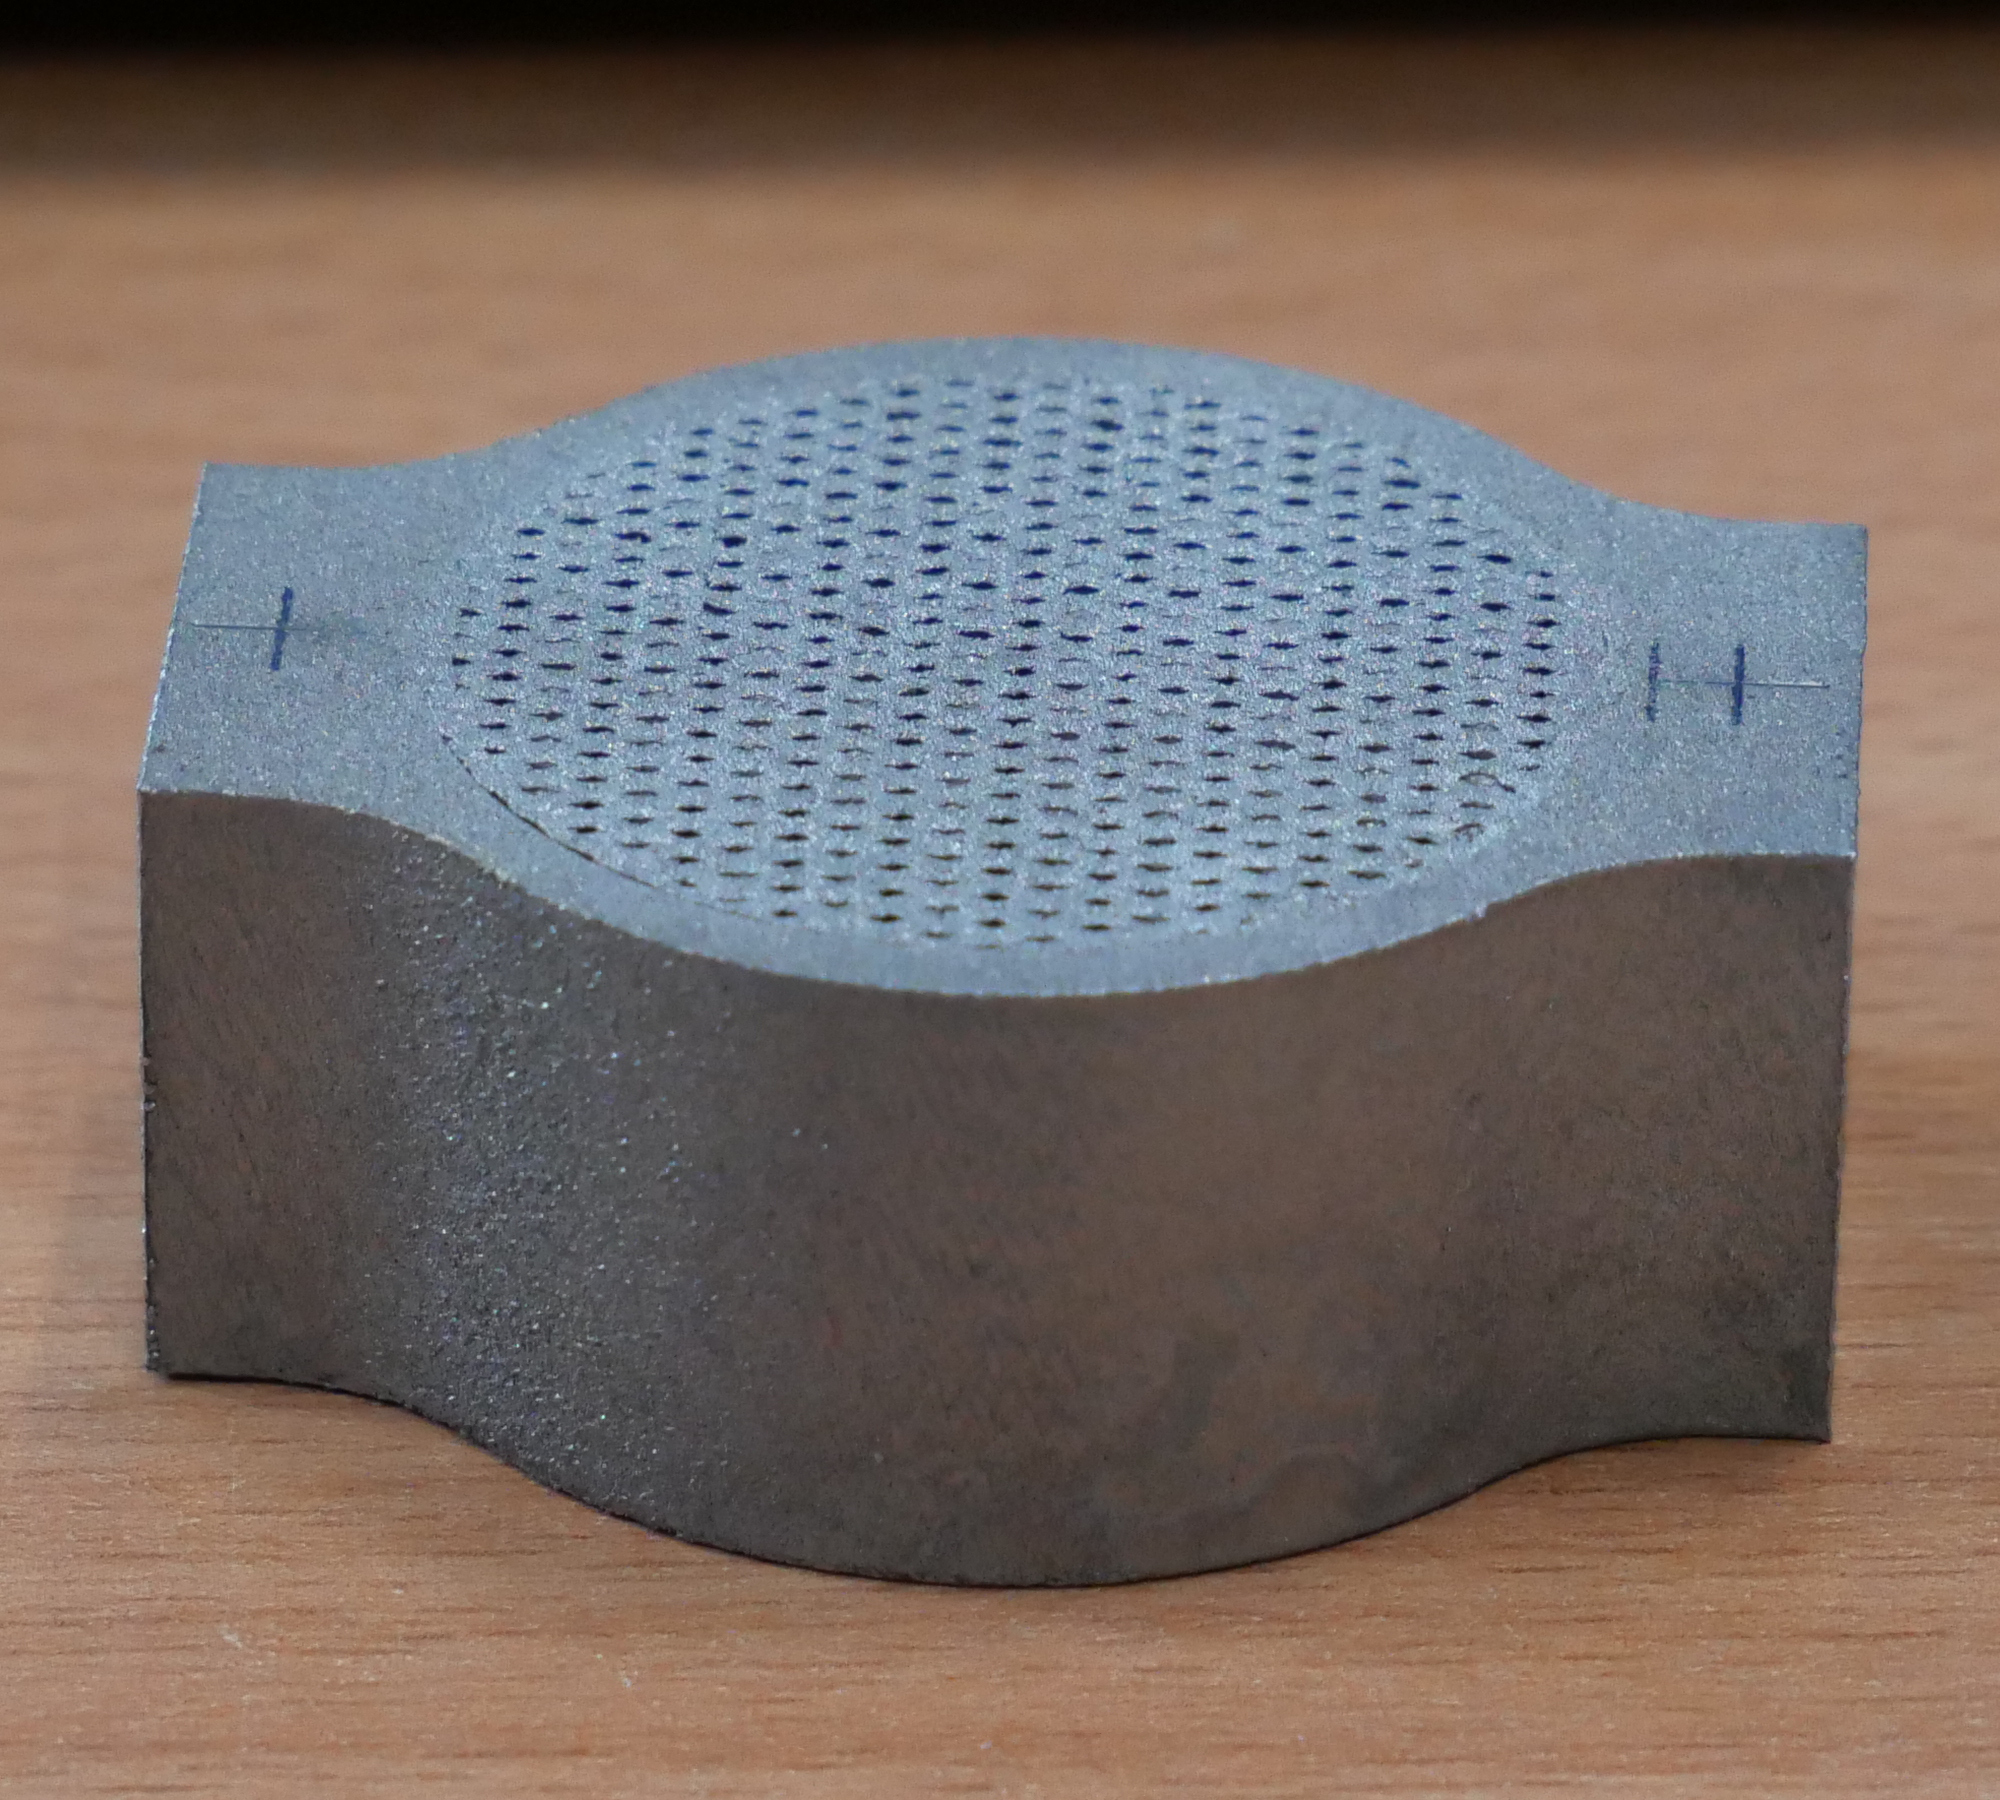
\includegraphics[width=0.9\linewidth]{images/AM0_crop.JPG}
      \caption*{(a)}
    \end{minipage}%
    \begin{minipage}{.33\textwidth}
      \centering
      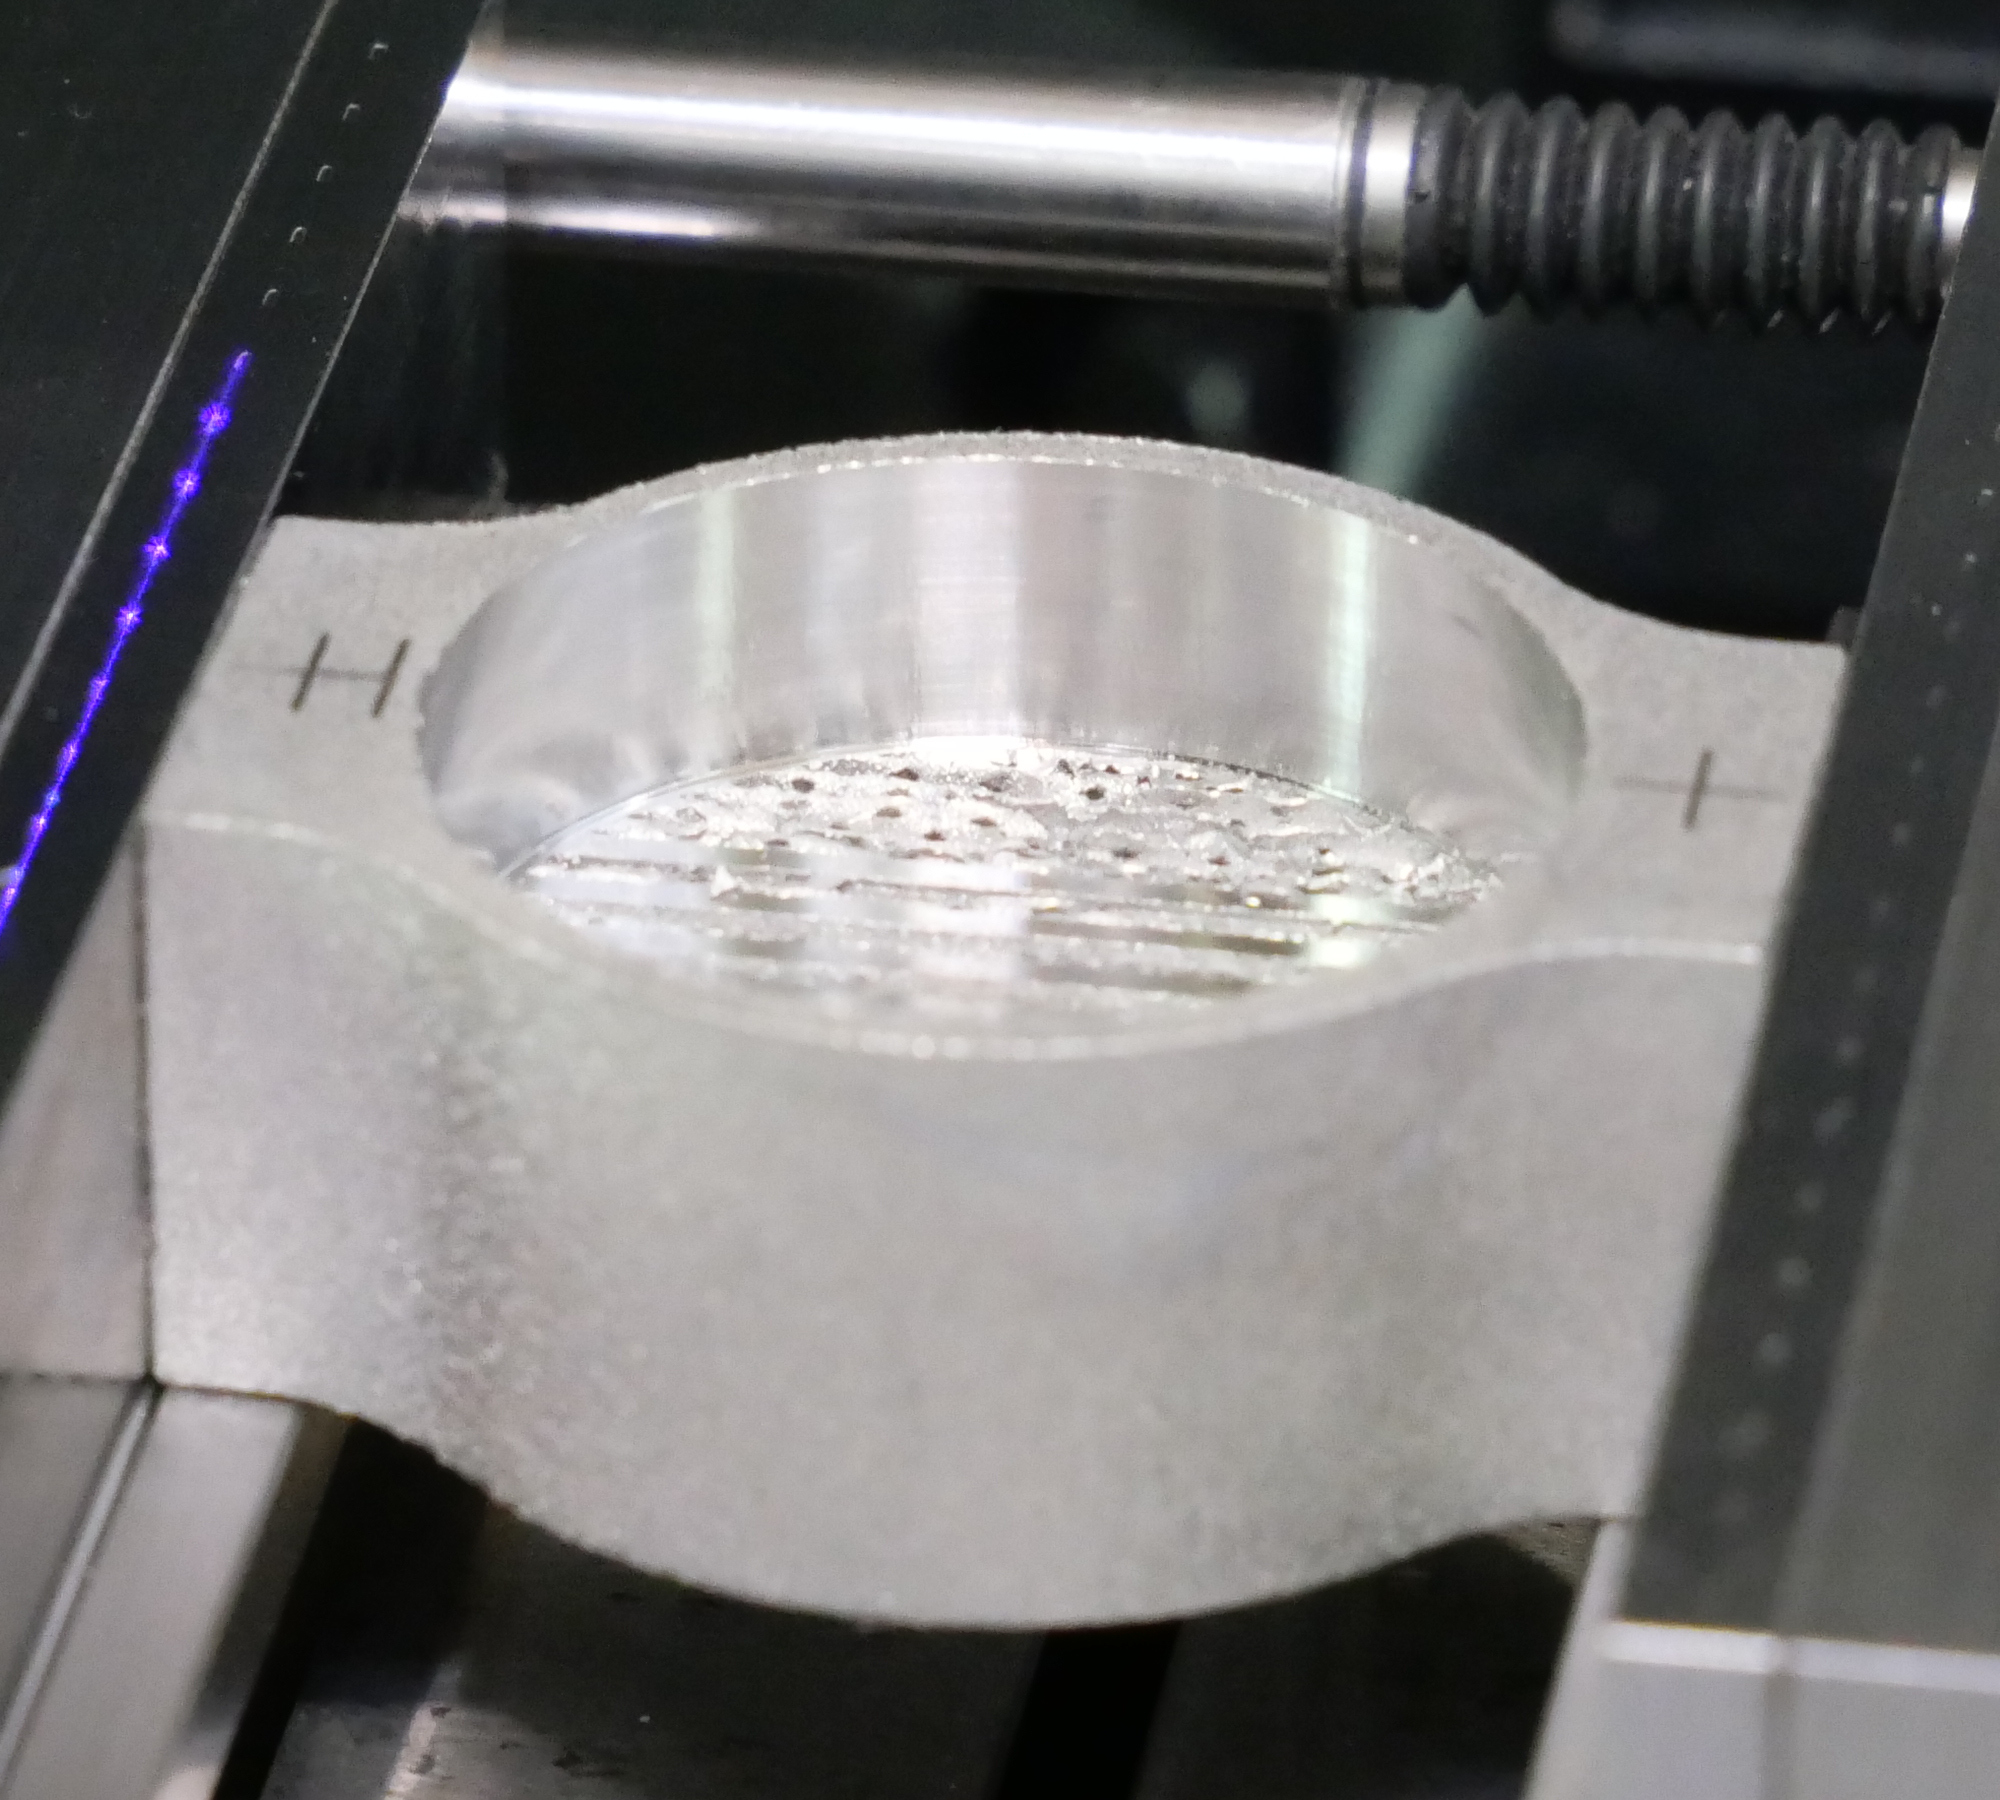
\includegraphics[width=0.9\linewidth]{images/AM1_crop.JPG}
      \caption*{(b)}
    \end{minipage}
    \begin{minipage}{.33\textwidth}
        \centering
        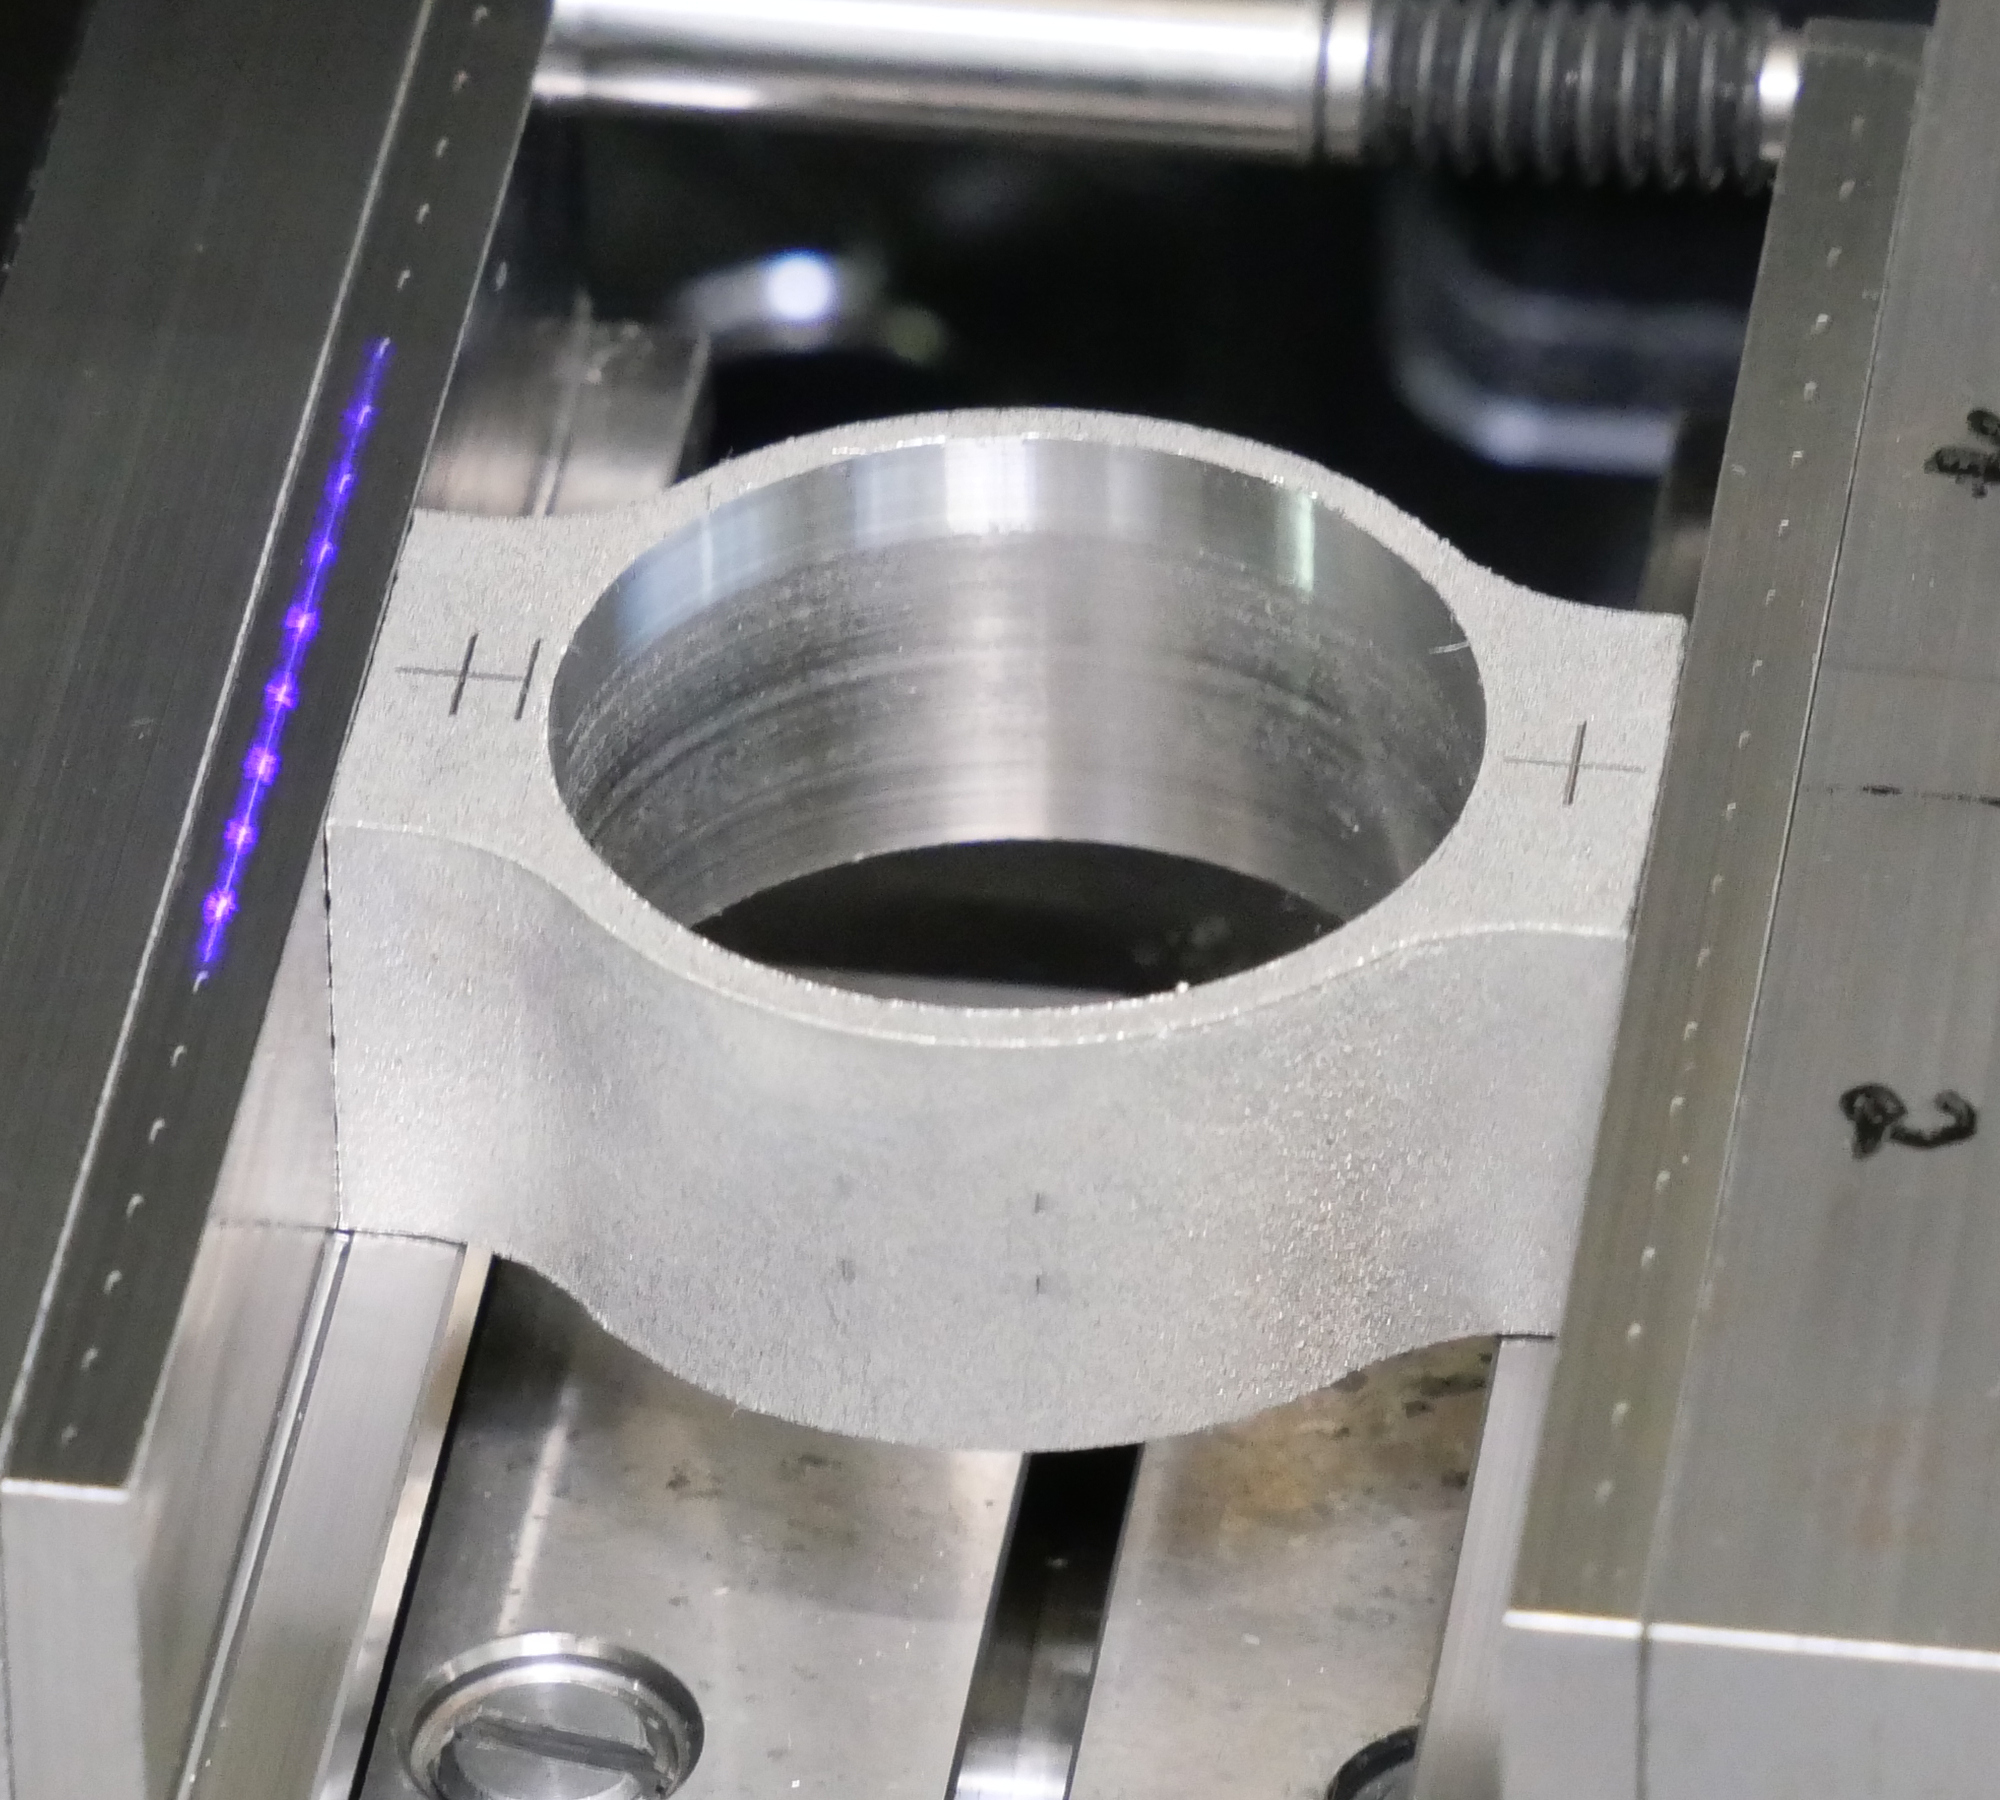
\includegraphics[width=0.9\linewidth]{images/AM2_crop.JPG}
        \caption*{(c)}
      \end{minipage}
      \caption{(a): AF Metallbauteil mit voller Stützstruktur, Bezeichnung: AM0.
      (b): AF Bauteil mit der halben Stützstruktur ausgebohrt, Bezeichnung: AM1.
      (c): AF Bauteil ohne Stützstruktur, Bezeichnung: AM2}
      \label{fig:am_parts}
\end{figure}

\section{Ergebnisse der optischen Deformationsanalyse}

In Abbildung \ref{fig:am_defos} und Abbildung \ref{fig:fdm_defos} sind die erkannten,
vertikalen Deformation grafisch dargestellt. Jeweils von Spannungsstufe null bis 
Spannungsstufen Sechs. Bei dem FDM Bauteil fehlt die Spannungsstufen fünf, 
diese ist leider bei der händischen Dateiname Vergabe überschrieben worden und konnte 
deshalb nicht ausgewertet worden. Aus diesem Grund ist eine so große Lücke in der 
Abbildung \ref{fig:fdm_defos}.
Außerdem sind große Unterschiede in der absoluten Deformation zu sehen. Zum Beispiel 
die rote Kurve in Abbildung \ref{fig:am_defos} die den Unterschied der Spannungsstufen 
null und eins angibt. Diese Kurve sollte näher an null der y-Achse liegen. 
Dies liegt an Ungenauigkeiten in dem Stitching Verfahren. In den Graphen ist also 
auf die Steigung der Deformationskurve zu achten. In der Steigung erkannt man das 
sich die Bauteile in mittleren Bereich nach außen hin deformiert haben und in 
den Randbereichen sich nach innen und dann wieder nach außen deformieren.
Außerdem ist im Vergleich der beiden Graphen zu sehen das sich das FDM Bauteil deutlich 
mehr verformt hat. Hier beträgt die größte Deformation über 150 Pixel.
Bei dem Metallbauteil, das mit der zehnfachen Kraft eingespannt wurde (250 nm vs. 2500 nm)
sind es nur knapp 40 Pixel, wie in Abbildung~\ref{fig:deformation_data_am} zu sehen. Trotzdem ist zu sehen das sich die Bauteile, die auch die 
gleiche Geometrie teilen, auf die gleiche Weise verformt haben.

\begin{figure}[H]
  \centering
  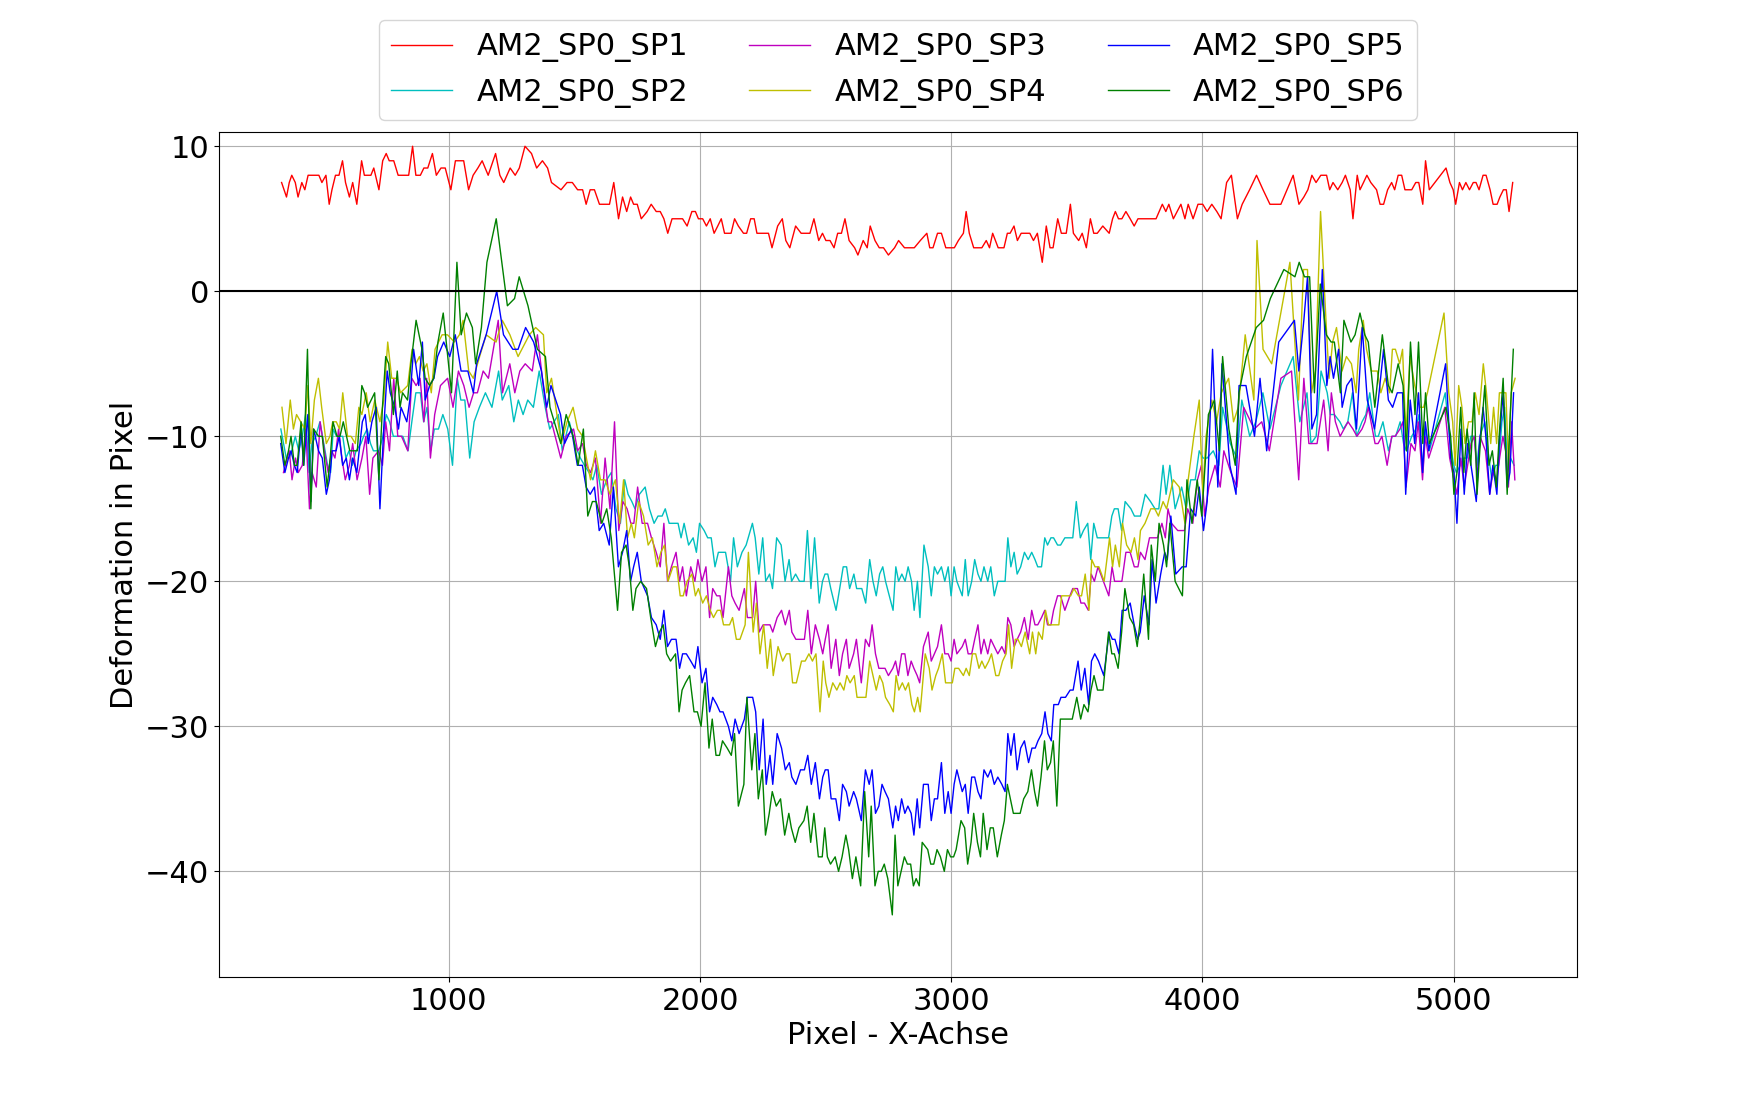
\includegraphics[width=0.95\textwidth]{images/am2_all_defos.png}
  \caption{Sechs Deformationsstufen bei einem additiv gefertigten Metallbauteil ohne
  Stützstruktur von 0 bis 2500 nm}
  \label{fig:am_defos}
\end{figure}

\begin{figure}[H]
  \centering
  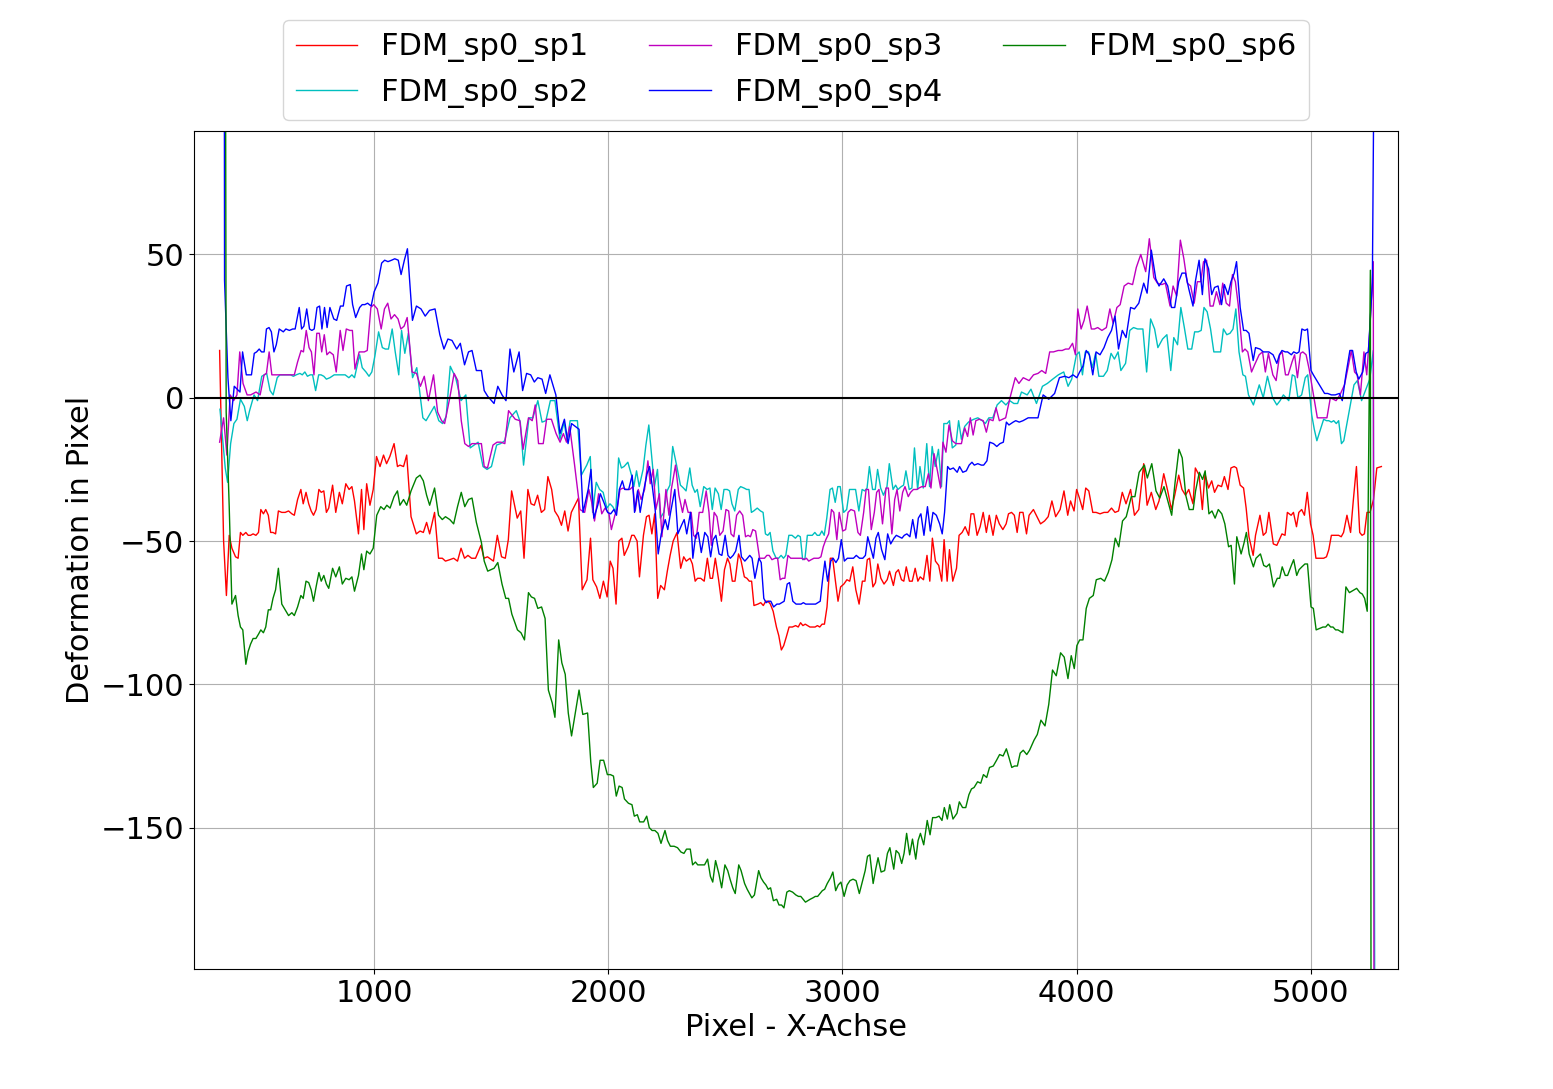
\includegraphics[width=0.95\textwidth]{images/fdm2_all_defos.png}
  \caption{Fünf Deformationsstufen bei einem FDM Bauteil von 0 bis 250 nm}
  \label{fig:fdm_defos}
\end{figure}

\begin{figure}[H]
    \centering
    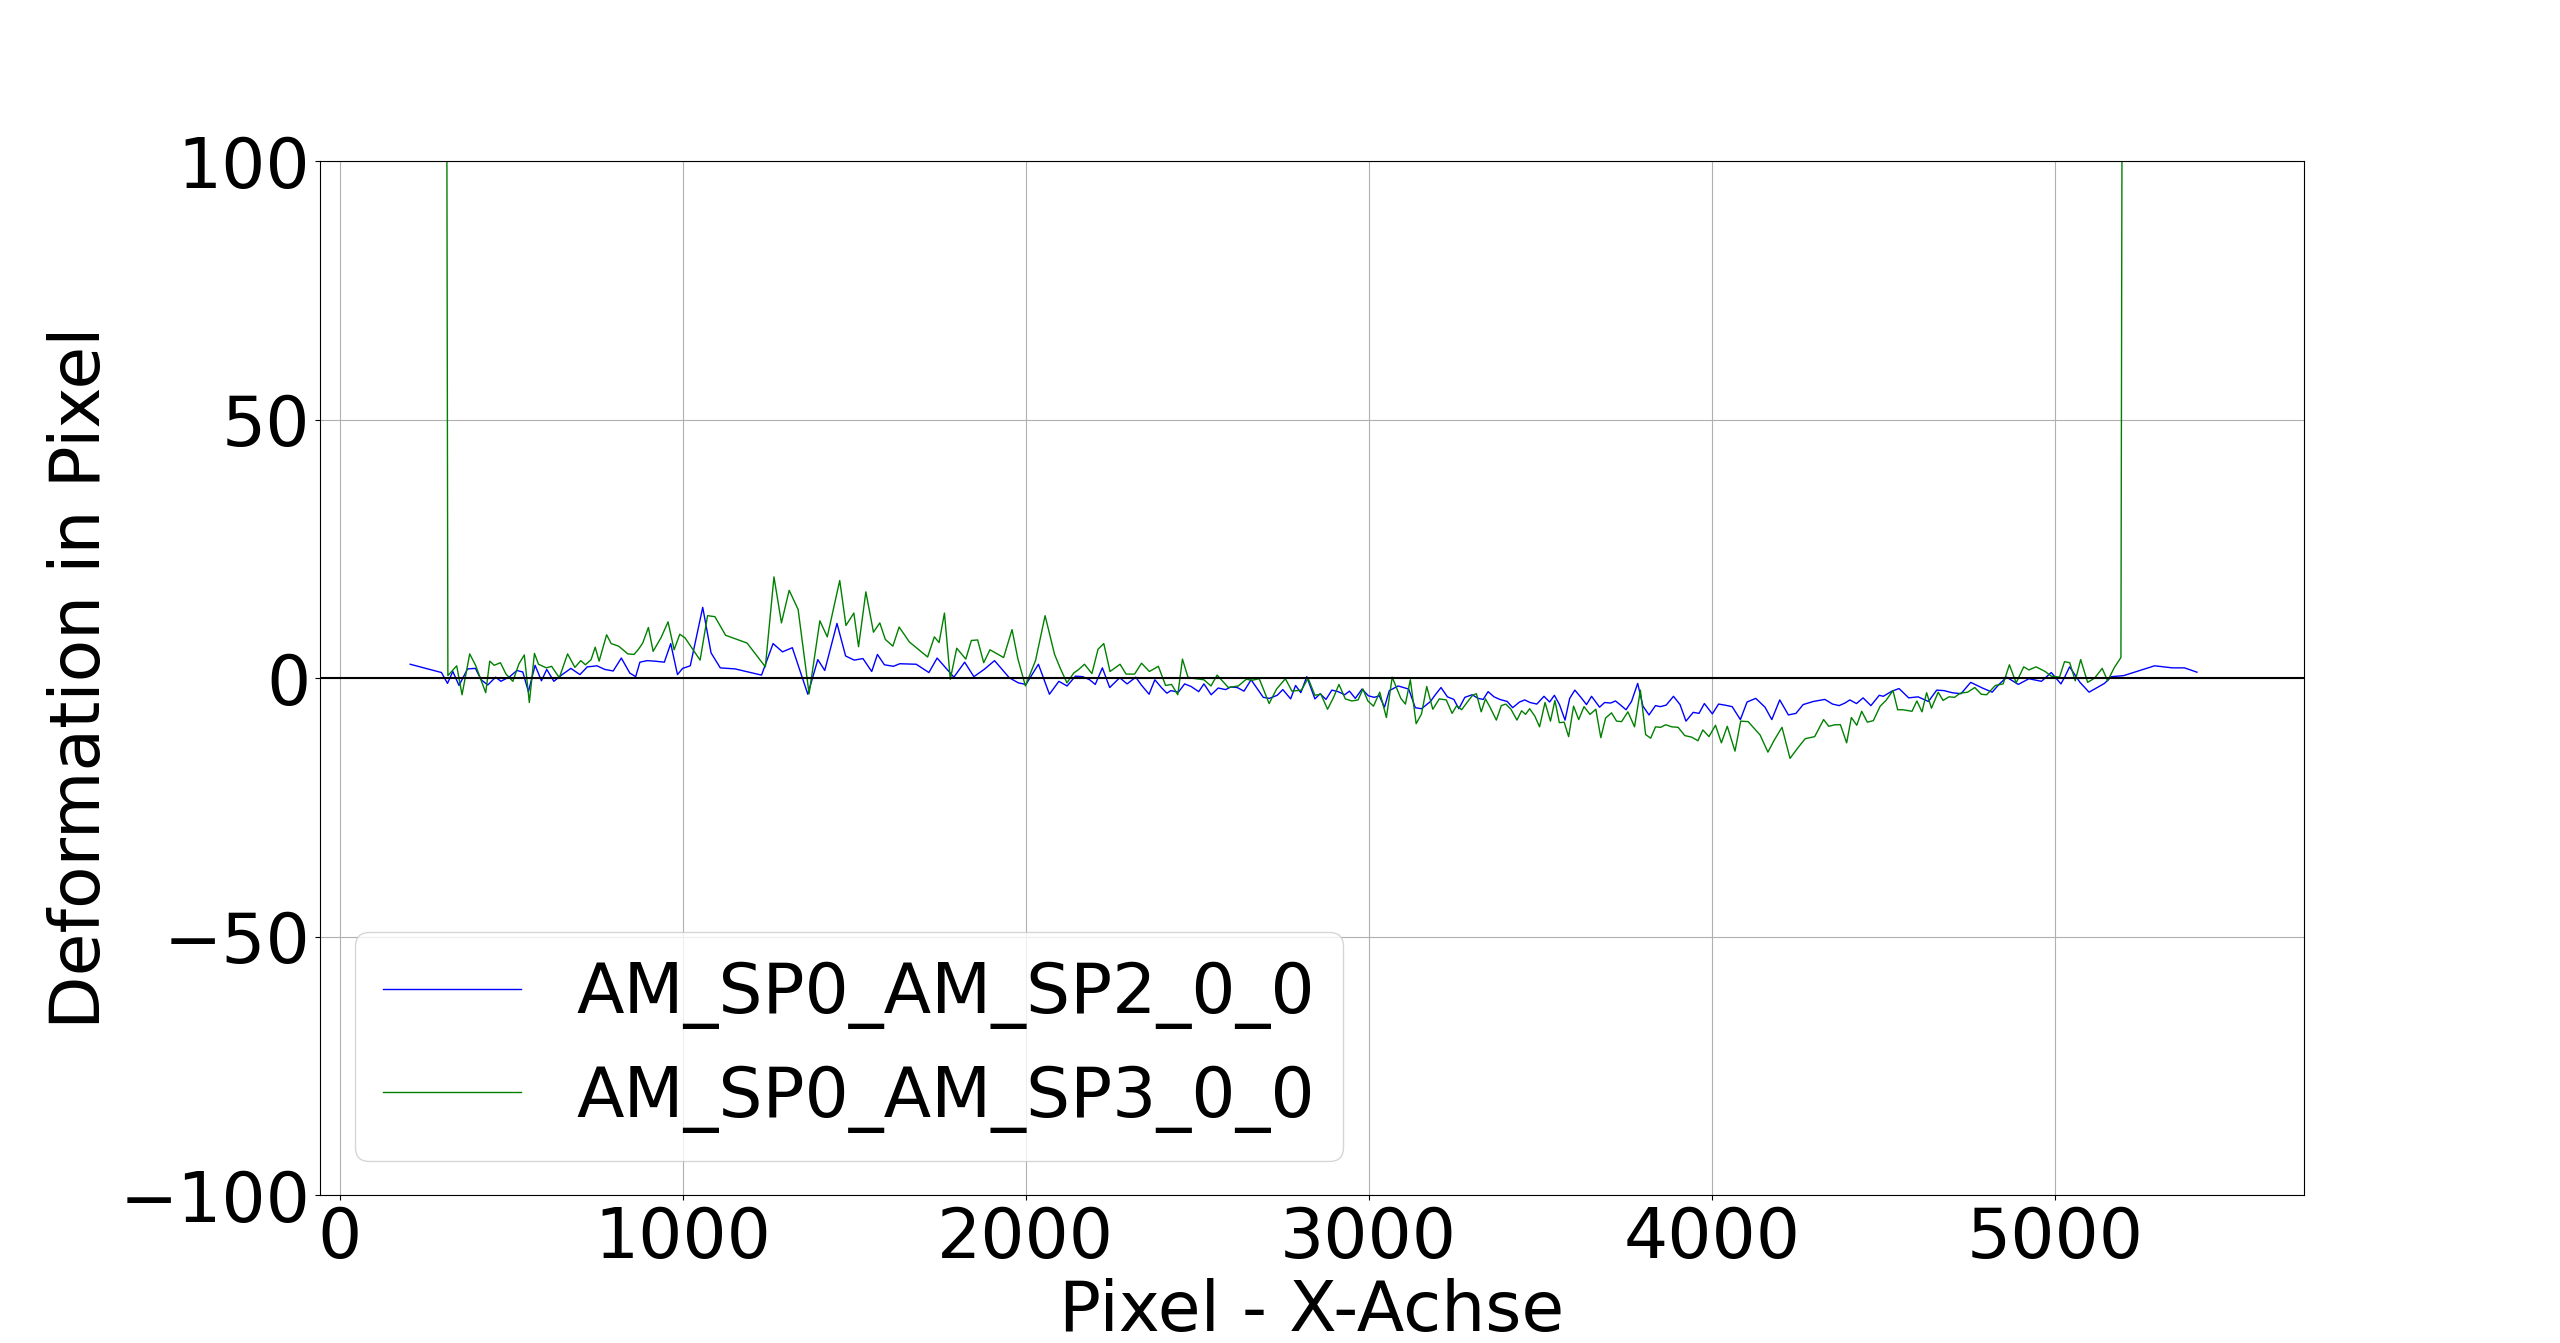
\includegraphics[width=0.9\textwidth]{images/AM_sp0_sp2_defo_plot.png}
    \caption{Differenz von zwei Spannungsstufen bei einem additiv gefertigten Metallbauteil, 
    das zur Hälfte mit Stützstrukturen gefüllt ist (Abbildung~\ref{fig:am_parts (b)}). }
    \label{fig:deformation_data_am}
\end{figure}

\section{Beurteilung der Ergebnisse}

Grundsätzlich ermöglicht die Methode die Erkennung und den Vergleich von Deformationen 
eines Bauteils. Die gemessene Deformation eines Bauteils entspricht den erwarteten Werten, 
abhängig von Material und Geometrie des Bauteils. FDM-gedruckte Kunststoffteile zeigen 
eine deutlich stärkere Verformung im Vergleich zu Metallteilen.
Bei den Metallteilen zeigt sich, dass das Vorhandensein einer Stützstruktur die
Verformung des Bauteils signifikant reduziert. 
Die unterschiedlichen Deformationen sind in Abbildung \ref{fig:materials} dargestellt. 
Das in Abbildung \ref{fig:am_parts} (a) gezeigte Bauteil konnte nicht analysiert werden, 
da durch die Stützstruktur keine korrekte Transformation zur stitchen berechnet werden konnte.
Bei den FDM-Bauteilen ist festzustellen, dass sie sich deutlich stärker verformen 
als die Metallteile. Beide FDM-Bauteile zeigen eine ähnliche Verformungsausprägung, 
jedoch tritt die Deformation, trotz identischer Geometrie, an unterschiedlichen Stellen auf. 
Dies könnte auf Unterschiede im Druckprozess zurückzuführen sein. 
Diese Beobachtung zeigt einen weiteren Nutzen der Methodik: Sie ermöglicht
nicht nur die Bestimmung des Ausmaßes der Deformation, sondern auch die 
Identifikation von Schwachstellen innerhalb eines Bauteils, die zu einer erhöhten 
 
Deformation führen.

\begin{figure}[H]
  \centering
  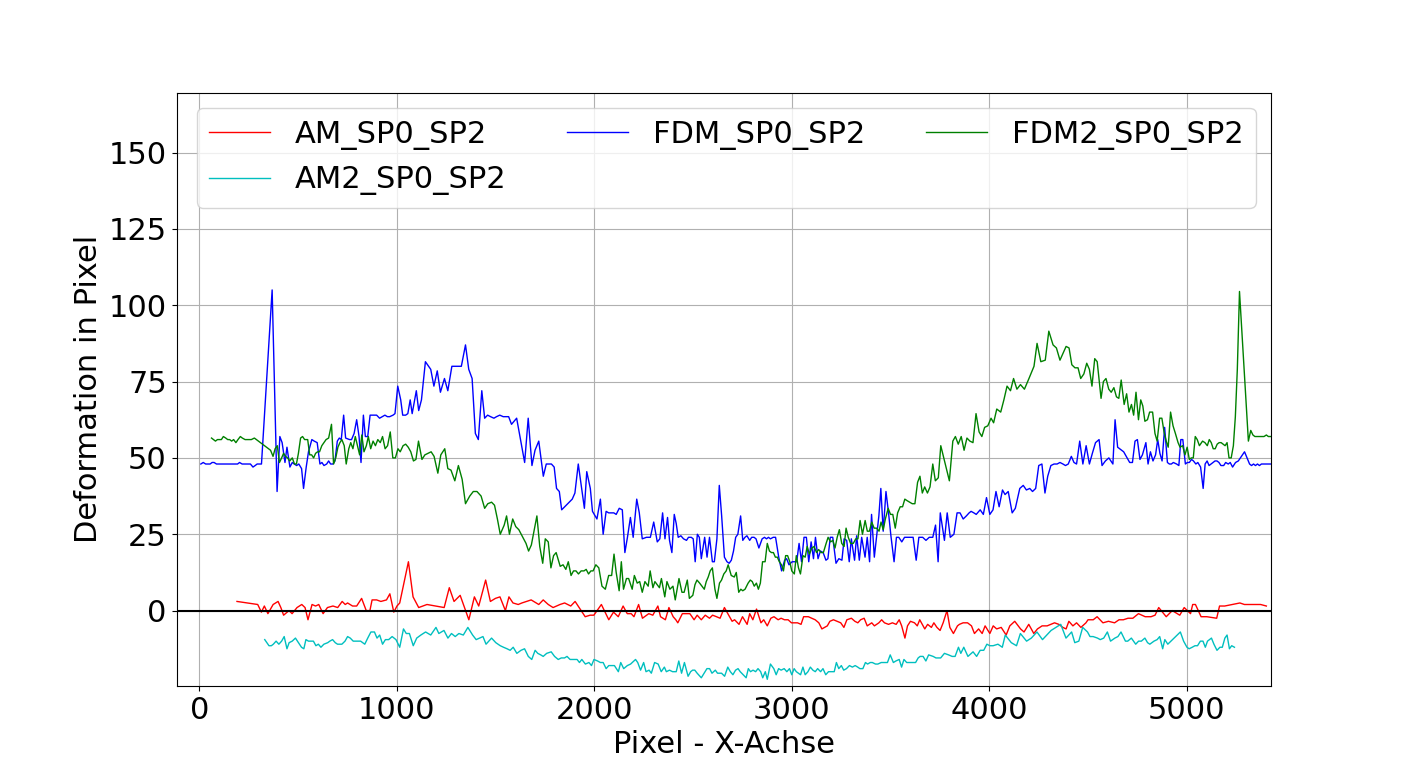
\includegraphics[width=0.95\textwidth]{images/compare_materials.png}
  \caption{Vergleich von Materialien und Bauteilgeometrien}
  \label{fig:materials}
\end{figure}

Dennoch ist die Deformationserkennung noch nicht perfekt. 
Fehler im Stitching Prozess führen zu starken Änderungen in der Deformationserkennung. 
Wie in Abbildung \ref{fig:errors} zu sehen ist, kann sich die Breite des Bauteils 
zwischen zwei Spannungsstufen unterscheiden. Er ist erkennbar, dass der Rand der einen 
Kontur, repräsentiert durch die magenta gefärbte Linie, immer größer ist als 
der Rand der anderen Kontur, hier in blau dargestellt.
Dieser Versatz entsteht, weil beim Stitching eine Transformation verwendet wurde die sich 
um wenige Pixel unterscheidet. Dadurch wächst auch die erkannte Deformationen.
Aus diesem Grund existieren in den Abbildungen \ref{fig:am_defos} und \ref{fig:fdm_defos}
Linien die nicht dem erwarteten Verhalten entsprechen. 
In Abbildung \ref{fig:fdm_defos} zum Beispiel, sollte die Deformation zwischen den 
Spannungsstufen eins und zwei 
(in rot dargestellt) am kleinsten sein. Stattdessen liegt die Kurve bei -50 Pixeln im Graph.

\begin{figure}[H]
  \centering
  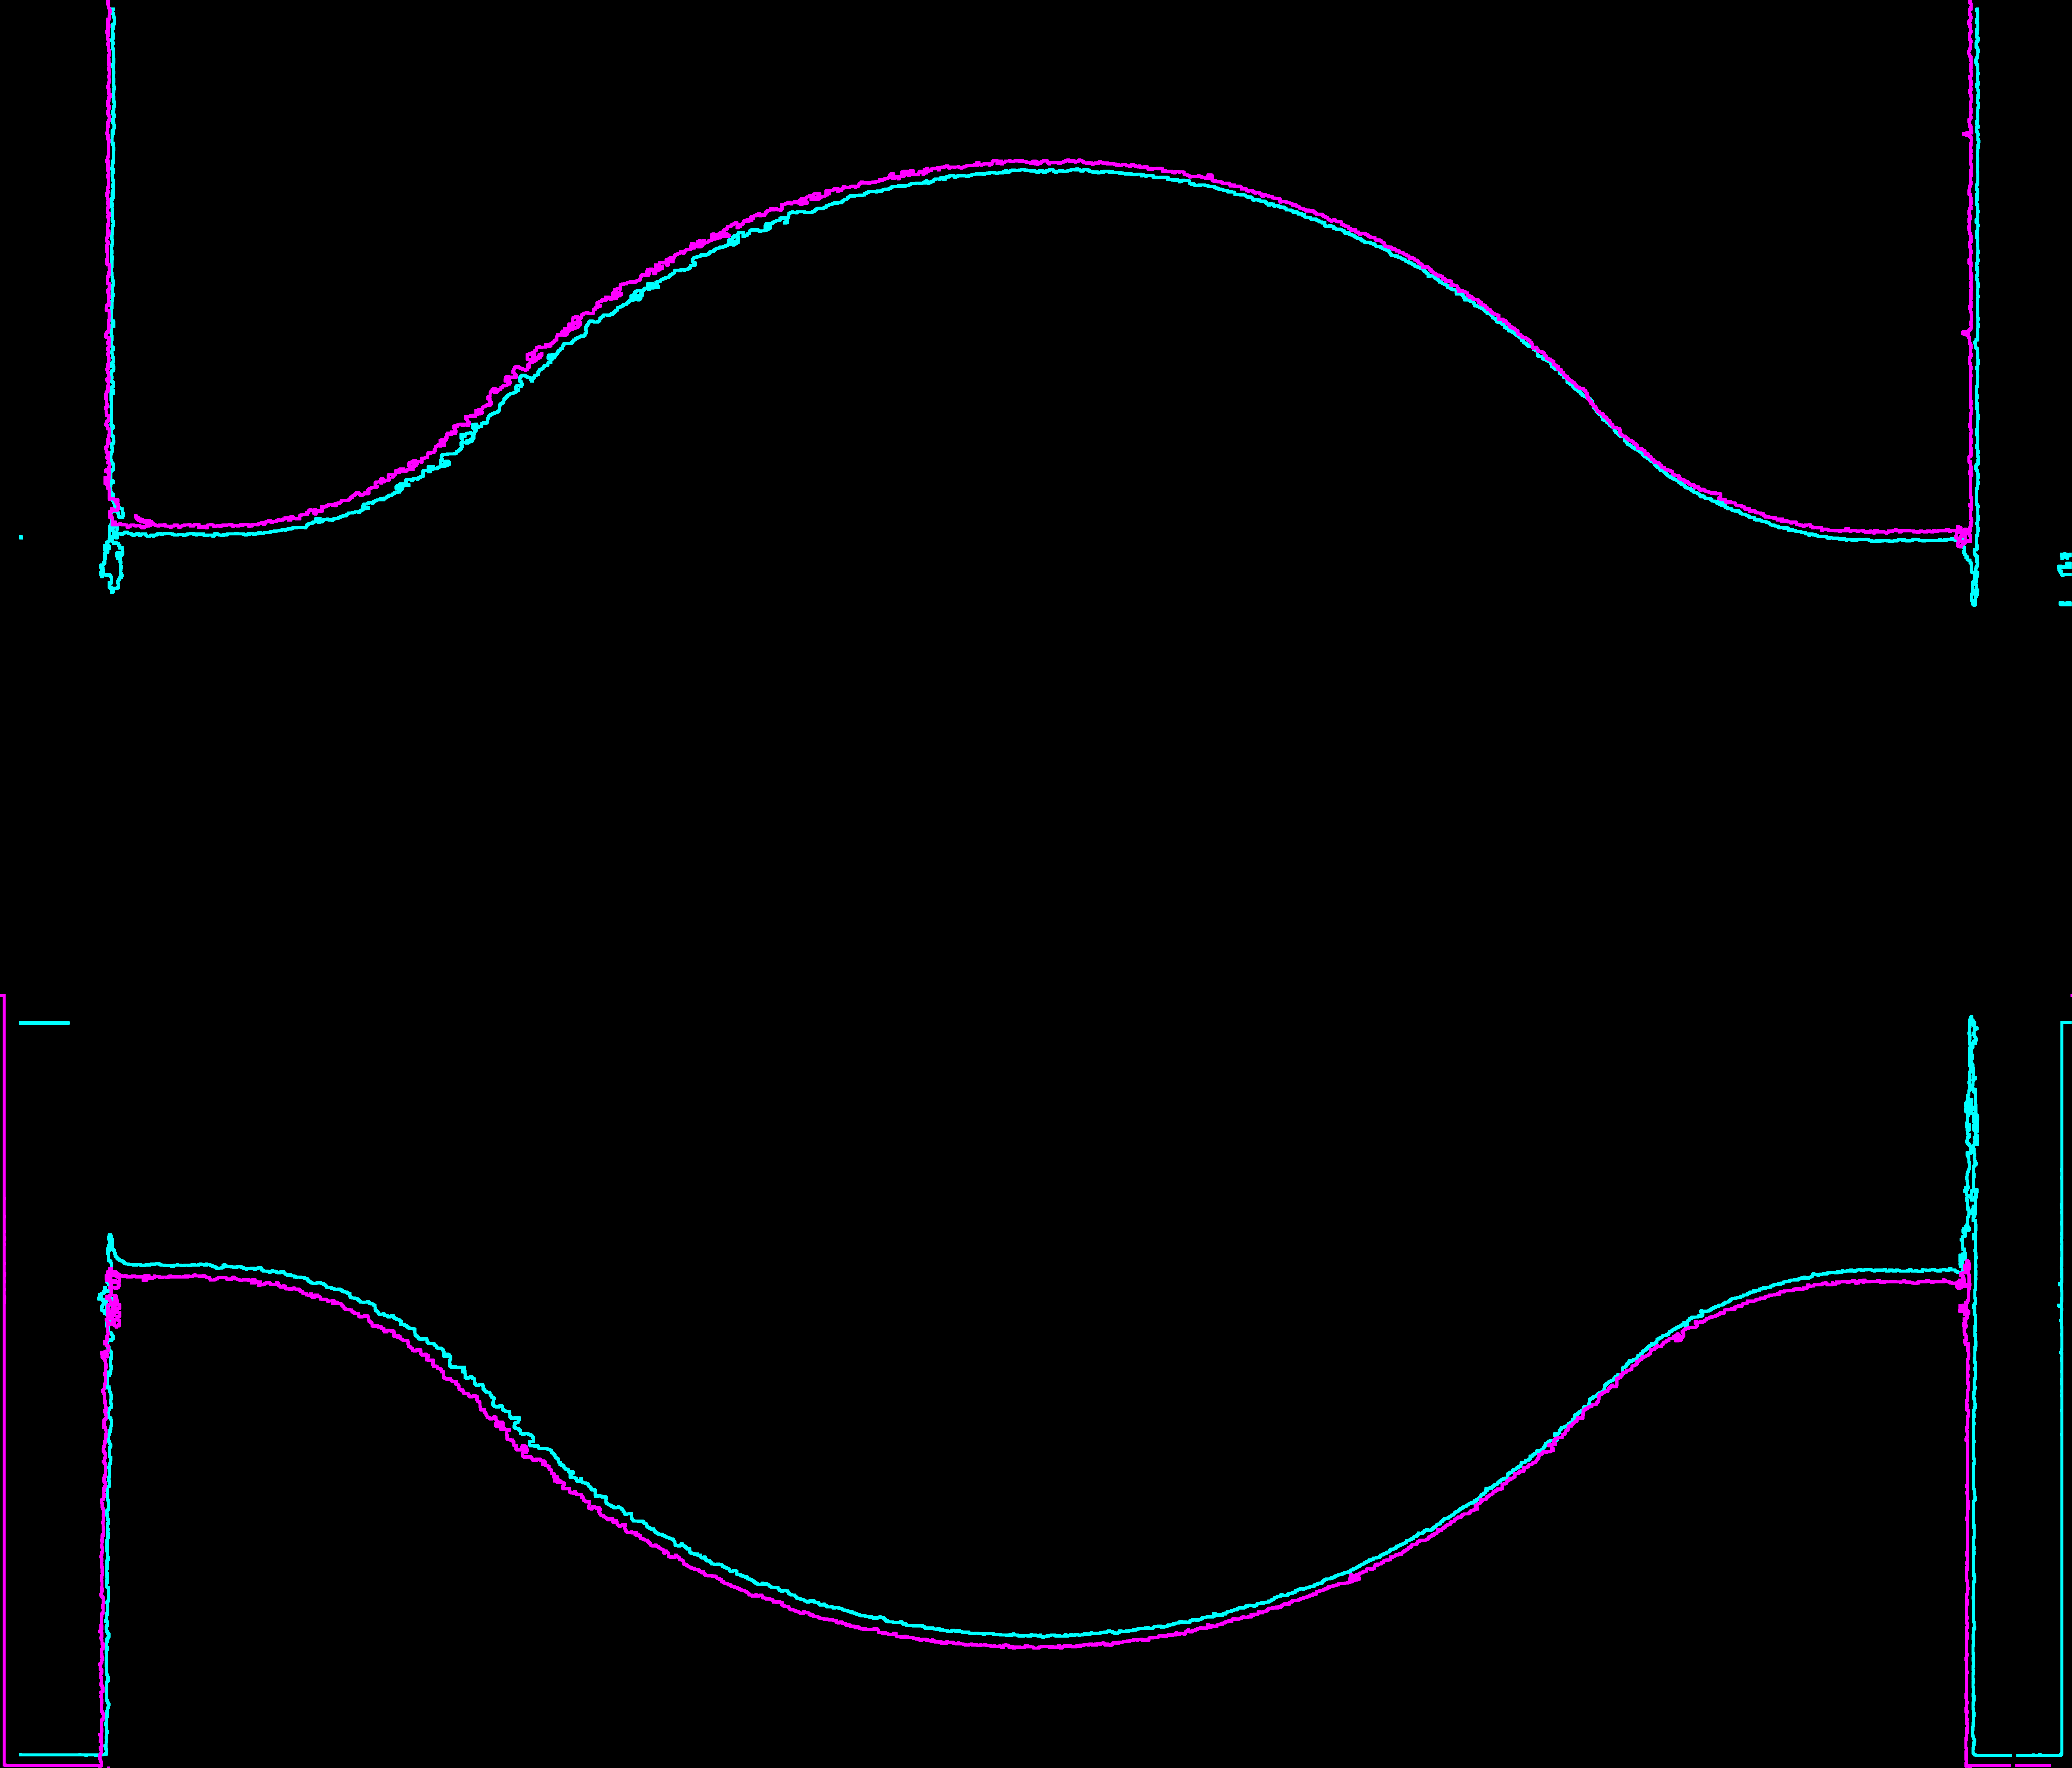
\includegraphics[width=0.95\textwidth]{images/contours_matching_36.png}
  \caption{Vergleich von Konturen aus nicht korrekt zusammengefügten Bildern.}
  \label{fig:errors}
\end{figure}

Zusätzlich kann, bei Bildern ohne klare Konturen, das Stitching nicht korrekt durchgeführt
werden. Dies ist bei den additiv gefertigten Metallbauteil mit Stützstruktur der Fall 
(Abbildung \ref{fig:am_parts} (a)). Das Bild, das aus dem Scan dieses Bauteils erstellt wurde, 
ist in Abbildung \ref{fig:errorimage} zu sehen. Es lassen sich keine eindeutigen Konturen 
erkennen, die für das Stitching genutzt werden könnten.

\begin{figure}[H]
  \centering
  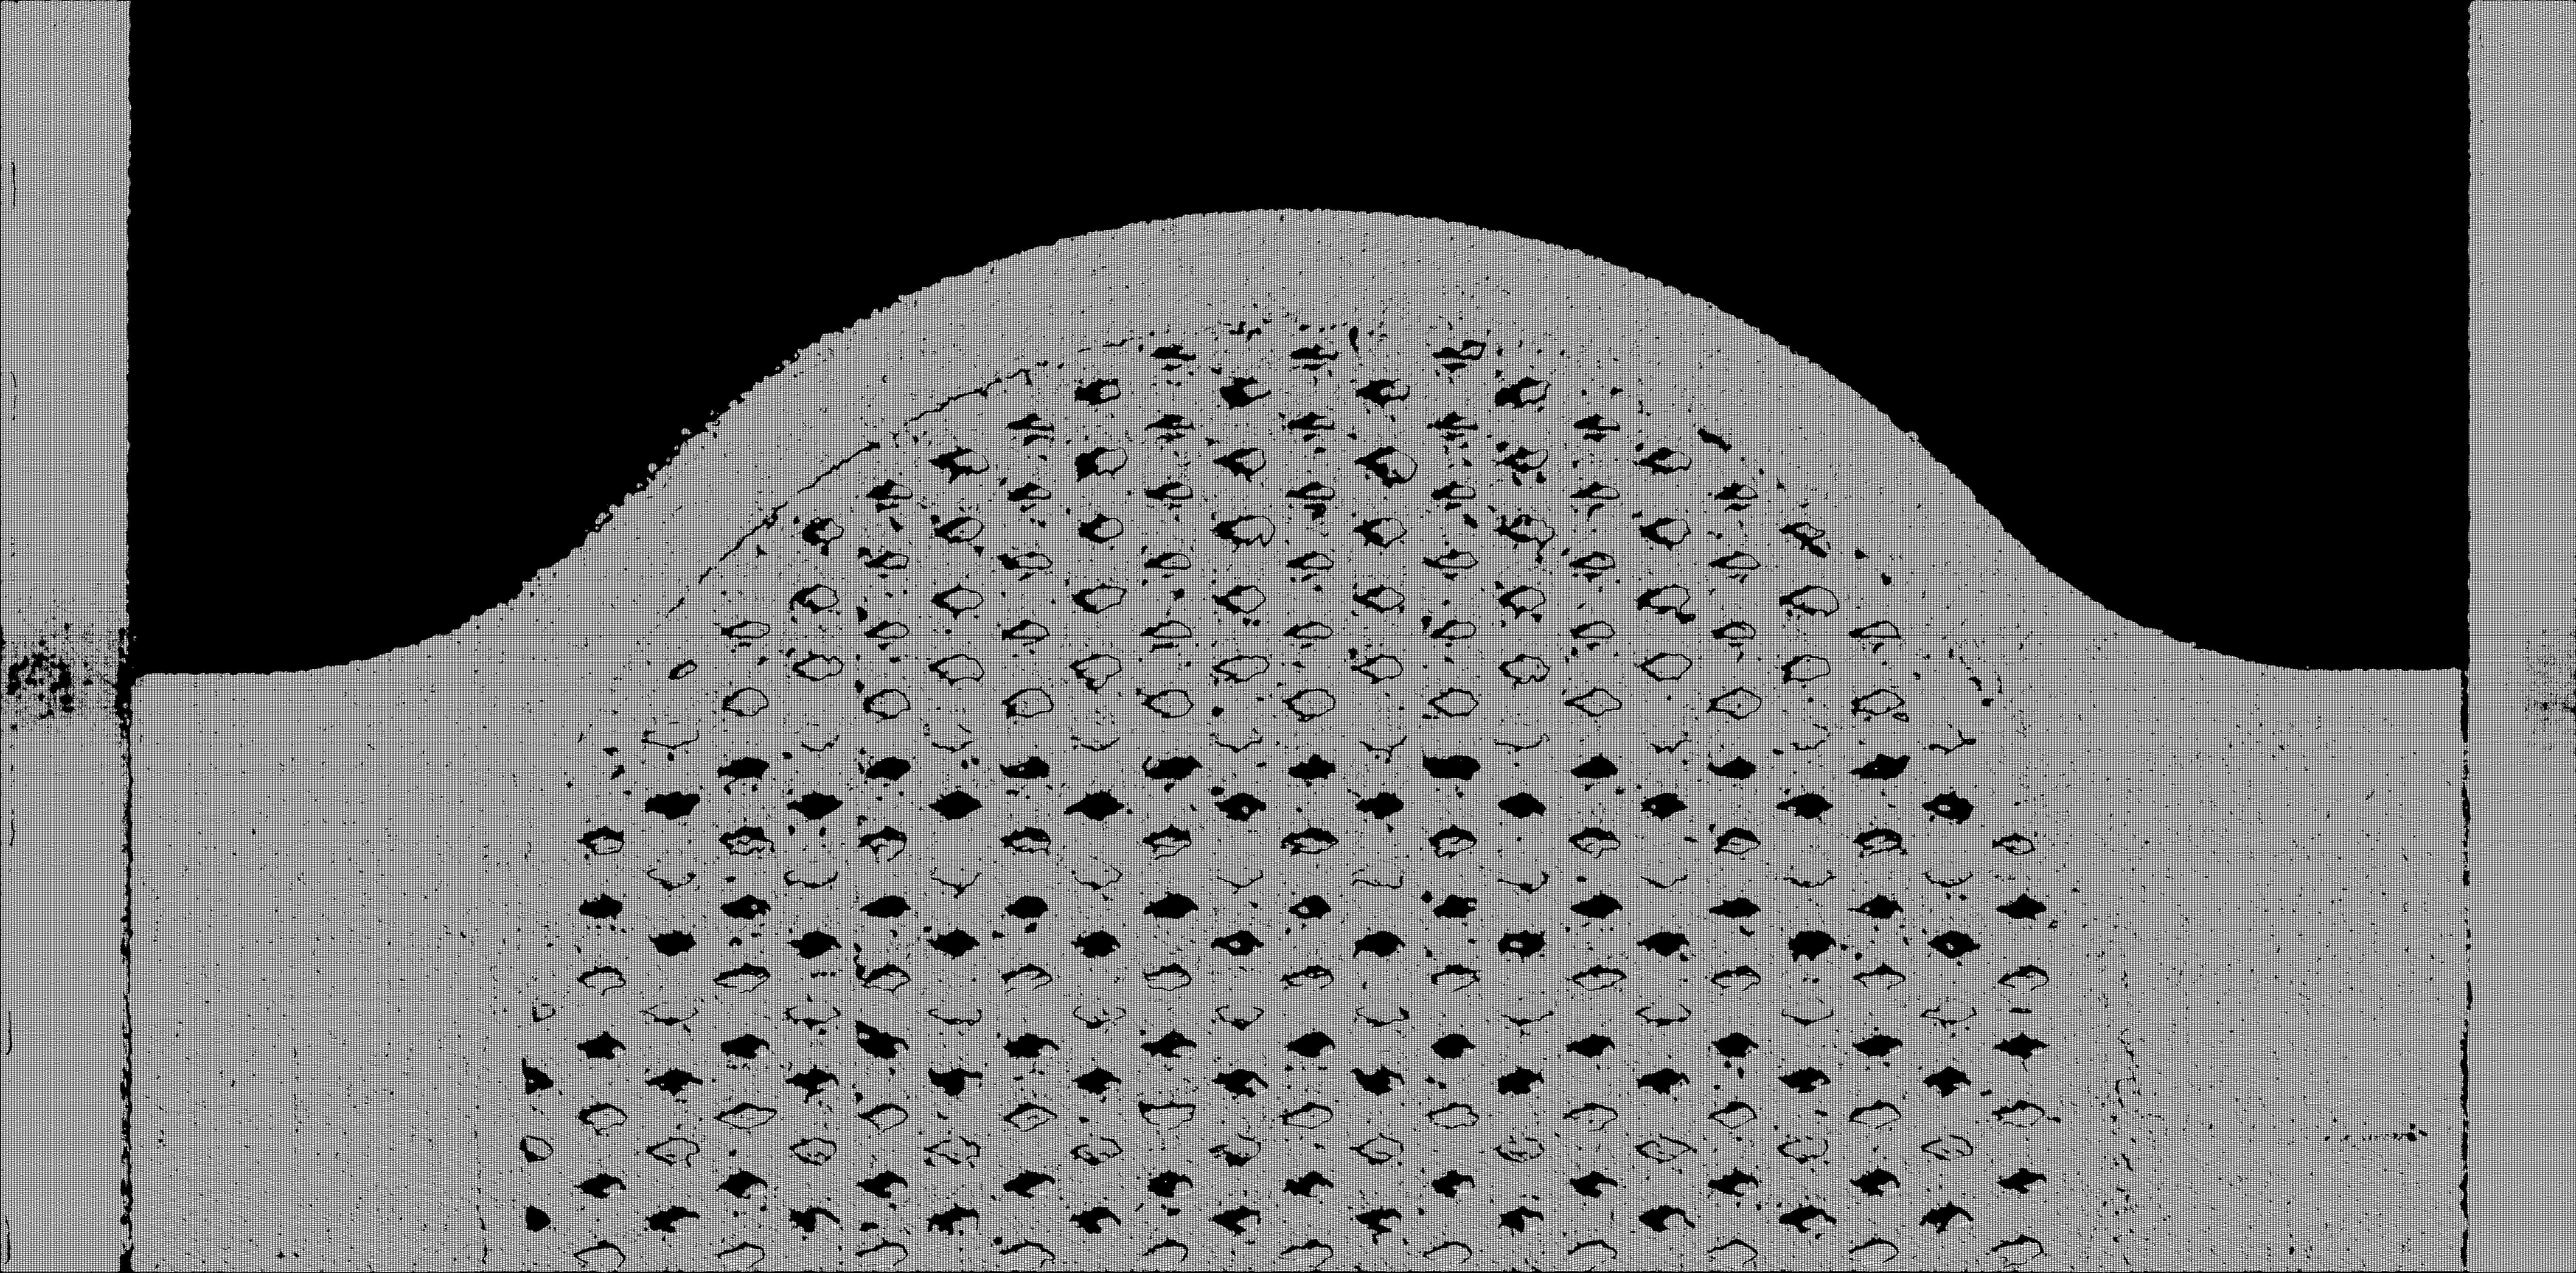
\includegraphics[width=0.95\textwidth]{images/am0.png}
  \caption{Bild eines Scans von einem Metallbauteil mit Stützstruktur.}
  \label{fig:errorimage}
\end{figure}



\documentclass[../main.tex]{subfiles}
\begin{document}

\section{Zusammenfassung und Ausblick}


\end{document}
% Anhang
\appendix
% Abbildungsverzeichnis
\listoffigures
\addcontentsline{toc}{chapter}{Abbildungsverzeichnis}
\cleardoublepage
% Algorithmenverzeichnis
\listofalgorithms
\addcontentsline{toc}{chapter}{Algorithmenverzeichnis}
\cleardoublepage
% Literaturverzeichnis
\bibliographystyle{alpha}
\bibliography{literatur/quellen}
\addcontentsline{toc}{chapter}{\bibname}
% Erklaerung
\thispagestyle{myheadings}
\markboth{}{ERKLÄRUNG}
\addcontentsline{toc}{chapter}{Erklärung}
% erklaerung.tex
\cleardoublepage
\Large
\noindent
\textbf{\affidavittitle}\\
\normalsize
\iflanguage{german}{Hiermit versichere ich, dass ich die vorliegende Arbeit selbstständig verfasst habe und keine anderen als die angegebenen Quellen und Hilfsmittel verwendet sowie Zitate kenntlich gemacht habe.\\\\	Dortmund, den \today}
{I herby declare that I created this thesis on my own, using only the sources mentioned. All Citations have been marked as such.\\\\ Dortmund, \today} \\\\\\\\
\nameofauthor
% EOF
\cleardoublepage
\end{document}

